\documentclass[a4paper]{book}
\usepackage{a4wide}
\usepackage{makeidx}
\usepackage{graphicx}
\usepackage{multicol}
\usepackage{float}
\usepackage{listings}
\usepackage{color}
\usepackage{textcomp}
\usepackage{alltt}
\usepackage{times}
\usepackage{ifpdf}
\ifpdf
\usepackage[pdftex,
            pagebackref=true,
            colorlinks=true,
            linkcolor=blue,
            unicode
           ]{hyperref}
\else
\usepackage[ps2pdf,
            pagebackref=true,
            colorlinks=true,
            linkcolor=blue,
            unicode
           ]{hyperref}
\usepackage{pspicture}
\fi
\usepackage[utf8]{inputenc}
\usepackage{doxygen}
\lstset{language=C++,inputencoding=utf8,basicstyle=\footnotesize,breaklines=true,breakatwhitespace=true,tabsize=8,numbers=left }
\makeindex
\setcounter{tocdepth}{3}
\renewcommand{\footrulewidth}{0.4pt}
\begin{document}
\hypersetup{pageanchor=false}
\begin{titlepage}
\vspace*{7cm}
\begin{center}
{\Large Heidelberg Educational Numerics Library \\[1ex]\large Version 0.23 (from 14 June 2011) }\\
\vspace*{1cm}
{\large Generated by Doxygen 1.6.3}\\
\vspace*{0.5cm}
{\small Tue Aug 30 15:55:38 2011}\\
\end{center}
\end{titlepage}
\clearemptydoublepage
\pagenumbering{roman}
\tableofcontents
\clearemptydoublepage
\pagenumbering{arabic}
\hypersetup{pageanchor=true}
\chapter{Class Index}
\section{Class Hierarchy}
This inheritance list is sorted roughly, but not completely, alphabetically:\begin{DoxyCompactList}
\item \contentsline{section}{hdnum::Array$<$ T $>$}{\pageref{classhdnum_1_1Array}}{}
\begin{DoxyCompactList}
\item \contentsline{section}{hdnum::CountableArray$<$ T $>$}{\pageref{classhdnum_1_1CountableArray}}{}
\end{DoxyCompactList}
\item \contentsline{section}{hdnum::Banach}{\pageref{classhdnum_1_1Banach}}{}
\item \contentsline{section}{hdnum::Countable}{\pageref{classhdnum_1_1Countable}}{}
\begin{DoxyCompactList}
\item \contentsline{section}{hdnum::CountableArray$<$ T $>$}{\pageref{classhdnum_1_1CountableArray}}{}
\end{DoxyCompactList}
\item \contentsline{section}{hdnum::CountableException}{\pageref{classhdnum_1_1CountableException}}{}
\item \contentsline{section}{hdnum::CP$<$ T, P $>$}{\pageref{classhdnum_1_1CP}}{}
\item \contentsline{section}{hdnum::DeletingMemoryManagementPolicy}{\pageref{classhdnum_1_1DeletingMemoryManagementPolicy}}{}
\item \contentsline{section}{hdnum::DenseMatrix$<$ REAL $>$}{\pageref{classhdnum_1_1DenseMatrix}}{}
\item \contentsline{section}{hdnum::DIRK$<$ M, S $>$}{\pageref{classhdnum_1_1DIRK}}{}
\item \contentsline{section}{hdnum::EE$<$ M $>$}{\pageref{classhdnum_1_1EE}}{}
\item \contentsline{section}{hdnum::Exception}{\pageref{classhdnum_1_1Exception}}{}
\begin{DoxyCompactList}
\item \contentsline{section}{hdnum::ErrorException}{\pageref{classhdnum_1_1ErrorException}}{}
\item \contentsline{section}{hdnum::InvalidStateException}{\pageref{classhdnum_1_1InvalidStateException}}{}
\item \contentsline{section}{hdnum::IOError}{\pageref{classhdnum_1_1IOError}}{}
\item \contentsline{section}{hdnum::MathError}{\pageref{classhdnum_1_1MathError}}{}
\item \contentsline{section}{hdnum::NotImplemented}{\pageref{classhdnum_1_1NotImplemented}}{}
\item \contentsline{section}{hdnum::RangeError}{\pageref{classhdnum_1_1RangeError}}{}
\item \contentsline{section}{hdnum::SystemError}{\pageref{classhdnum_1_1SystemError}}{}
\begin{DoxyCompactList}
\item \contentsline{section}{hdnum::OutOfMemoryError}{\pageref{classhdnum_1_1OutOfMemoryError}}{}
\item \contentsline{section}{hdnum::TimerError}{\pageref{classhdnum_1_1TimerError}}{}
\end{DoxyCompactList}
\end{DoxyCompactList}
\item \contentsline{section}{hdnum::Heun2$<$ M $>$}{\pageref{classhdnum_1_1Heun2}}{}
\item \contentsline{section}{hdnum::Heun3$<$ M $>$}{\pageref{classhdnum_1_1Heun3}}{}
\item \contentsline{section}{hdnum::IE$<$ M, S $>$}{\pageref{classhdnum_1_1IE}}{}
\item \contentsline{section}{hdnum::Kutta3$<$ M $>$}{\pageref{classhdnum_1_1Kutta3}}{}
\item \contentsline{section}{hdnum::Matrix$<$ T $>$}{\pageref{classhdnum_1_1Matrix}}{}
\item \contentsline{section}{hdnum::ModifiedEuler$<$ M $>$}{\pageref{classhdnum_1_1ModifiedEuler}}{}
\item \contentsline{section}{hdnum::Newton}{\pageref{classhdnum_1_1Newton}}{}
\item \contentsline{section}{hdnum::NondeletingMemoryManagementPolicy}{\pageref{classhdnum_1_1NondeletingMemoryManagementPolicy}}{}
\item \contentsline{section}{hdnum::RE$<$ M, S $>$}{\pageref{classhdnum_1_1RE}}{}
\item \contentsline{section}{hdnum::RKF45$<$ M $>$}{\pageref{classhdnum_1_1RKF45}}{}
\item \contentsline{section}{hdnum::RungeKutta4$<$ M $>$}{\pageref{classhdnum_1_1RungeKutta4}}{}
\item \contentsline{section}{hdnum::SGrid$<$ N, DF, dimension $>$}{\pageref{classhdnum_1_1SGrid}}{}
\item \contentsline{section}{hdnum::SquareRootProblem$<$ N $>$}{\pageref{classhdnum_1_1SquareRootProblem}}{}
\item \contentsline{section}{hdnum::StationarySolver$<$ M $>$}{\pageref{classhdnum_1_1StationarySolver}}{}
\item \contentsline{section}{hdnum::Timer}{\pageref{classhdnum_1_1Timer}}{}
\item \contentsline{section}{vector}{\pageref{classstd_1_1vector}}{}
\item \contentsline{section}{hdnum::Vector$<$ REAL $>$}{\pageref{classhdnum_1_1Vector}}{}
\end{DoxyCompactList}

\chapter{Class Index}
\section{Class List}
Here are the classes, structs, unions and interfaces with brief descriptions:\begin{DoxyCompactList}
\item\contentsline{section}{\hyperlink{classhdnum_1_1Array}{hdnum::Array$<$ T $>$} (A basic dynamic array class )}{\pageref{classhdnum_1_1Array}}{}
\item\contentsline{section}{\hyperlink{classhdnum_1_1Banach}{hdnum::Banach} (Solve nonlinear problem using a fixed point iteration )}{\pageref{classhdnum_1_1Banach}}{}
\item\contentsline{section}{\hyperlink{classhdnum_1_1Countable}{hdnum::Countable} (Base class for object pointed to by \hyperlink{classhdnum_1_1CP}{CP} )}{\pageref{classhdnum_1_1Countable}}{}
\item\contentsline{section}{\hyperlink{classhdnum_1_1CountableArray}{hdnum::CountableArray$<$ T $>$} (Dynamic array that can be used with the reference counting pointer )}{\pageref{classhdnum_1_1CountableArray}}{}
\item\contentsline{section}{\hyperlink{classhdnum_1_1CountableException}{hdnum::CountableException} }{\pageref{classhdnum_1_1CountableException}}{}
\item\contentsline{section}{\hyperlink{classhdnum_1_1CP}{hdnum::CP$<$ T, P $>$} (Pointer with a reference count in the pointed-\/to object )}{\pageref{classhdnum_1_1CP}}{}
\item\contentsline{section}{\hyperlink{classhdnum_1_1DeletingMemoryManagementPolicy}{hdnum::DeletingMemoryManagementPolicy} (Delete target if reference count reaches zero )}{\pageref{classhdnum_1_1DeletingMemoryManagementPolicy}}{}
\item\contentsline{section}{\hyperlink{classhdnum_1_1DenseMatrix}{hdnum::DenseMatrix$<$ REAL $>$} (Class with mathematical matrix operations )}{\pageref{classhdnum_1_1DenseMatrix}}{}
\item\contentsline{section}{\hyperlink{classhdnum_1_1DIRK}{hdnum::DIRK$<$ M, S $>$} (Implementation of a general Diagonal Implicit Runge-\/Kutta method )}{\pageref{classhdnum_1_1DIRK}}{}
\item\contentsline{section}{\hyperlink{classhdnum_1_1EE}{hdnum::EE$<$ M $>$} (Explicit Euler method as an example for an ODE solver )}{\pageref{classhdnum_1_1EE}}{}
\item\contentsline{section}{\hyperlink{classhdnum_1_1ErrorException}{hdnum::ErrorException} (General Error )}{\pageref{classhdnum_1_1ErrorException}}{}
\item\contentsline{section}{\hyperlink{classhdnum_1_1Exception}{hdnum::Exception} (Base class for Exceptions )}{\pageref{classhdnum_1_1Exception}}{}
\item\contentsline{section}{\hyperlink{classhdnum_1_1Heun2}{hdnum::Heun2$<$ M $>$} (Heun method (order 2 with 2 stages) )}{\pageref{classhdnum_1_1Heun2}}{}
\item\contentsline{section}{\hyperlink{classhdnum_1_1Heun3}{hdnum::Heun3$<$ M $>$} (Heun method (order 3 with 3 stages) )}{\pageref{classhdnum_1_1Heun3}}{}
\item\contentsline{section}{\hyperlink{classhdnum_1_1IE}{hdnum::IE$<$ M, S $>$} (Implicit Euler using Newton's method to solve nonlinear system )}{\pageref{classhdnum_1_1IE}}{}
\item\contentsline{section}{\hyperlink{classhdnum_1_1InvalidStateException}{hdnum::InvalidStateException} (Default exception if a function was called while the object is not in a valid state for that function )}{\pageref{classhdnum_1_1InvalidStateException}}{}
\item\contentsline{section}{\hyperlink{classhdnum_1_1IOError}{hdnum::IOError} (Default exception class for I/O errors )}{\pageref{classhdnum_1_1IOError}}{}
\item\contentsline{section}{\hyperlink{classhdnum_1_1Kutta3}{hdnum::Kutta3$<$ M $>$} (Kutta method (order 3 with 3 stages) )}{\pageref{classhdnum_1_1Kutta3}}{}
\item\contentsline{section}{\hyperlink{classhdnum_1_1MathError}{hdnum::MathError} (Default exception class for mathematical errors )}{\pageref{classhdnum_1_1MathError}}{}
\item\contentsline{section}{\hyperlink{classhdnum_1_1Matrix}{hdnum::Matrix$<$ T $>$} (A flexible matrix class )}{\pageref{classhdnum_1_1Matrix}}{}
\item\contentsline{section}{\hyperlink{classhdnum_1_1ModifiedEuler}{hdnum::ModifiedEuler$<$ M $>$} (Modified Euler method (order 2 with 2 stages) )}{\pageref{classhdnum_1_1ModifiedEuler}}{}
\item\contentsline{section}{\hyperlink{classhdnum_1_1Newton}{hdnum::Newton} (Solve nonlinear problem using a damped \hyperlink{classhdnum_1_1Newton}{Newton} method )}{\pageref{classhdnum_1_1Newton}}{}
\item\contentsline{section}{\hyperlink{classhdnum_1_1NondeletingMemoryManagementPolicy}{hdnum::NondeletingMemoryManagementPolicy} (Don't delete target if reference count reaches zero )}{\pageref{classhdnum_1_1NondeletingMemoryManagementPolicy}}{}
\item\contentsline{section}{\hyperlink{classhdnum_1_1NotImplemented}{hdnum::NotImplemented} (Default exception for dummy implementations )}{\pageref{classhdnum_1_1NotImplemented}}{}
\item\contentsline{section}{\hyperlink{classhdnum_1_1OutOfMemoryError}{hdnum::OutOfMemoryError} (Default exception if memory allocation fails )}{\pageref{classhdnum_1_1OutOfMemoryError}}{}
\item\contentsline{section}{\hyperlink{classhdnum_1_1RangeError}{hdnum::RangeError} (Default exception class for range errors )}{\pageref{classhdnum_1_1RangeError}}{}
\item\contentsline{section}{\hyperlink{classhdnum_1_1RE}{hdnum::RE$<$ M, S $>$} (Adaptive one-\/step method using Richardson extrapolation )}{\pageref{classhdnum_1_1RE}}{}
\item\contentsline{section}{\hyperlink{classhdnum_1_1RKF45}{hdnum::RKF45$<$ M $>$} (Adaptive Runge-\/Kutta-\/Fehlberg method )}{\pageref{classhdnum_1_1RKF45}}{}
\item\contentsline{section}{\hyperlink{classhdnum_1_1RungeKutta4}{hdnum::RungeKutta4$<$ M $>$} (Classical Runge-\/Kutta method (order 4 with 4 stages) )}{\pageref{classhdnum_1_1RungeKutta4}}{}
\item\contentsline{section}{\hyperlink{classhdnum_1_1SGrid}{hdnum::SGrid$<$ N, DF, dimension $>$} (Structured Grid for Finite Differences )}{\pageref{classhdnum_1_1SGrid}}{}
\item\contentsline{section}{\hyperlink{classhdnum_1_1SquareRootProblem}{hdnum::SquareRootProblem$<$ N $>$} (Example class for a nonlinear model F(x) = 0; )}{\pageref{classhdnum_1_1SquareRootProblem}}{}
\item\contentsline{section}{\hyperlink{classhdnum_1_1StationarySolver}{hdnum::StationarySolver$<$ M $>$} (Stationary problem solver. E.g. for elliptic problmes )}{\pageref{classhdnum_1_1StationarySolver}}{}
\item\contentsline{section}{\hyperlink{classhdnum_1_1SystemError}{hdnum::SystemError} (Default exception class for OS errors )}{\pageref{classhdnum_1_1SystemError}}{}
\item\contentsline{section}{\hyperlink{classhdnum_1_1Timer}{hdnum::Timer} (A simple stop watch )}{\pageref{classhdnum_1_1Timer}}{}
\item\contentsline{section}{\hyperlink{classhdnum_1_1TimerError}{hdnum::TimerError} (Exception thrown by the \hyperlink{classhdnum_1_1Timer}{Timer} class )}{\pageref{classhdnum_1_1TimerError}}{}
\item\contentsline{section}{\hyperlink{classstd_1_1vector}{vector} }{\pageref{classstd_1_1vector}}{}
\item\contentsline{section}{\hyperlink{classhdnum_1_1Vector}{hdnum::Vector$<$ REAL $>$} (Class with mathematical vector operations )}{\pageref{classhdnum_1_1Vector}}{}
\end{DoxyCompactList}

\chapter{File Index}
\section{File List}
Here is a list of all documented files with brief descriptions:\begin{DoxyCompactList}
\item\contentsline{section}{src/\hyperlink{array_8hh}{array.hh} (This file implements a basic dynamic array class )}{\pageref{array_8hh}}{}
\item\contentsline{section}{src/\hyperlink{countablearray_8hh}{countablearray.hh} (This file implements a basic dynamic array class )}{\pageref{countablearray_8hh}}{}
\item\contentsline{section}{src/\hyperlink{countingptr_8hh}{countingptr.hh} (This file implements a counting pointer with configurable memory management policy Adapted from dune-\/pdelab )}{\pageref{countingptr_8hh}}{}
\item\contentsline{section}{src/{\bfseries densematrix.hh} }{\pageref{densematrix_8hh}}{}
\item\contentsline{section}{src/\hyperlink{exceptions_8hh}{exceptions.hh} (A few common exception classes )}{\pageref{exceptions_8hh}}{}
\item\contentsline{section}{src/\hyperlink{lr_8hh}{lr.hh} (This file implements a generic and dynamic vector class )}{\pageref{lr_8hh}}{}
\item\contentsline{section}{src/\hyperlink{matrix_8hh}{matrix.hh} (This file implements a generic and dynamic matrix class )}{\pageref{matrix_8hh}}{}
\item\contentsline{section}{src/\hyperlink{newton_8hh}{newton.hh} (Newton's method with line search )}{\pageref{newton_8hh}}{}
\item\contentsline{section}{src/\hyperlink{ode_8hh}{ode.hh} (Solvers for ordinary differential equations )}{\pageref{ode_8hh}}{}
\item\contentsline{section}{src/\hyperlink{pde_8hh}{pde.hh} (Solvers for partial differential equations )}{\pageref{pde_8hh}}{}
\item\contentsline{section}{src/\hyperlink{precision_8hh}{precision.hh} (Find machine precision for given float type )}{\pageref{precision_8hh}}{}
\item\contentsline{section}{src/{\bfseries sgrid.hh} }{\pageref{sgrid_8hh}}{}
\item\contentsline{section}{src/\hyperlink{timer_8hh}{timer.hh} (A simple timing class )}{\pageref{timer_8hh}}{}
\item\contentsline{section}{src/{\bfseries vector.hh} }{\pageref{vector_8hh}}{}
\end{DoxyCompactList}

\chapter{Class Documentation}
\hypertarget{classhdnum_1_1Array}{
\section{hdnum::Array$<$ T $>$ Class Template Reference}
\label{classhdnum_1_1Array}\index{hdnum::Array@{hdnum::Array}}
}


A basic dynamic array class.  




{\ttfamily \#include $<$array.hh$>$}

Inheritance diagram for hdnum::Array$<$ T $>$:\begin{figure}[H]
\begin{center}
\leavevmode
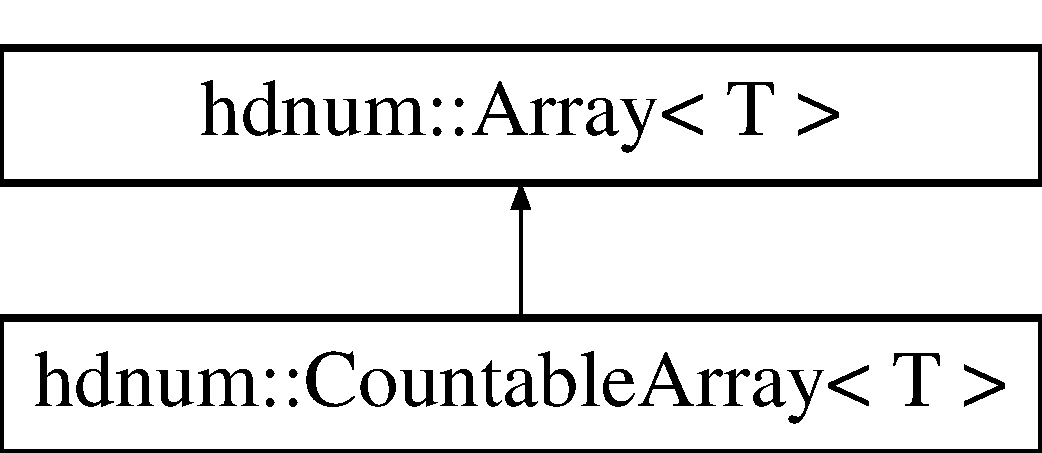
\includegraphics[height=2cm]{classhdnum_1_1Array}
\end{center}
\end{figure}
\subsection*{Public Types}
\begin{DoxyCompactItemize}
\item 
\hypertarget{classhdnum_1_1Array_ae77aae65dae609c72534babc774dd152}{
typedef T \hyperlink{classhdnum_1_1Array_ae77aae65dae609c72534babc774dd152}{value\_\-type}}
\label{classhdnum_1_1Array_ae77aae65dae609c72534babc774dd152}

\begin{DoxyCompactList}\small\item\em Remember the storage type. \item\end{DoxyCompactList}\item 
\hypertarget{classhdnum_1_1Array_a5c1db6b52b2f88c3618040f856bdcdbe}{
typedef \hyperlink{classhdnum_1_1Array_ae77aae65dae609c72534babc774dd152}{value\_\-type} \& \hyperlink{classhdnum_1_1Array_a5c1db6b52b2f88c3618040f856bdcdbe}{reference}}
\label{classhdnum_1_1Array_a5c1db6b52b2f88c3618040f856bdcdbe}

\begin{DoxyCompactList}\small\item\em Reference to an object. \item\end{DoxyCompactList}\item 
\hypertarget{classhdnum_1_1Array_ad696c724bcda975ea63492d0786a1509}{
typedef const \hyperlink{classhdnum_1_1Array_ae77aae65dae609c72534babc774dd152}{value\_\-type} \& \hyperlink{classhdnum_1_1Array_ad696c724bcda975ea63492d0786a1509}{const\_\-reference}}
\label{classhdnum_1_1Array_ad696c724bcda975ea63492d0786a1509}

\begin{DoxyCompactList}\small\item\em Const reference to an object. \item\end{DoxyCompactList}\item 
\hypertarget{classhdnum_1_1Array_a52bad04c045624e4240073f8efb2e8e1}{
typedef std::size\_\-t \hyperlink{classhdnum_1_1Array_a52bad04c045624e4240073f8efb2e8e1}{size\_\-type}}
\label{classhdnum_1_1Array_a52bad04c045624e4240073f8efb2e8e1}

\begin{DoxyCompactList}\small\item\em Type used for array indices. \item\end{DoxyCompactList}\item 
\hypertarget{classhdnum_1_1Array_abb53f0f2fda2009c75602e374de9c0d7}{
typedef std::ptrdiff\_\-t \hyperlink{classhdnum_1_1Array_abb53f0f2fda2009c75602e374de9c0d7}{difference\_\-type}}
\label{classhdnum_1_1Array_abb53f0f2fda2009c75602e374de9c0d7}

\begin{DoxyCompactList}\small\item\em Difference type. \item\end{DoxyCompactList}\end{DoxyCompactItemize}
\subsection*{Public Member Functions}
\begin{DoxyCompactItemize}
\item 
\hypertarget{classhdnum_1_1Array_a8ffcdc4e69b3ddc00d1ec97189436a57}{
\hyperlink{classhdnum_1_1Array_a8ffcdc4e69b3ddc00d1ec97189436a57}{Array} ()}
\label{classhdnum_1_1Array_a8ffcdc4e69b3ddc00d1ec97189436a57}

\begin{DoxyCompactList}\small\item\em make empty array \item\end{DoxyCompactList}\item 
\hypertarget{classhdnum_1_1Array_afa6e185e6b30e1ba0aeecfd86b5997f1}{
\hyperlink{classhdnum_1_1Array_afa6e185e6b30e1ba0aeecfd86b5997f1}{Array} (\hyperlink{classhdnum_1_1Array_a52bad04c045624e4240073f8efb2e8e1}{size\_\-type} \_\-n)}
\label{classhdnum_1_1Array_afa6e185e6b30e1ba0aeecfd86b5997f1}

\begin{DoxyCompactList}\small\item\em make array with \_\-n uninitialized components \item\end{DoxyCompactList}\item 
\hypertarget{classhdnum_1_1Array_ad7c595fddcdf74a8c768fdb3b63b6365}{
\hyperlink{classhdnum_1_1Array_ad7c595fddcdf74a8c768fdb3b63b6365}{Array} (\hyperlink{classhdnum_1_1Array_a52bad04c045624e4240073f8efb2e8e1}{size\_\-type} \_\-n, const T \&\_\-t)}
\label{classhdnum_1_1Array_ad7c595fddcdf74a8c768fdb3b63b6365}

\begin{DoxyCompactList}\small\item\em make array with \_\-n initialized components \item\end{DoxyCompactList}\item 
\hypertarget{classhdnum_1_1Array_a2f537b09e173003db9ef8ab0aa7d465c}{
\hyperlink{classhdnum_1_1Array_a2f537b09e173003db9ef8ab0aa7d465c}{Array} (const \hyperlink{classhdnum_1_1Array}{Array} \&a)}
\label{classhdnum_1_1Array_a2f537b09e173003db9ef8ab0aa7d465c}

\begin{DoxyCompactList}\small\item\em copy constructor \item\end{DoxyCompactList}\item 
\hypertarget{classhdnum_1_1Array_aafee3af74a03d909efa743e39360404c}{
\hyperlink{classhdnum_1_1Array_aafee3af74a03d909efa743e39360404c}{$\sim$Array} ()}
\label{classhdnum_1_1Array_aafee3af74a03d909efa743e39360404c}

\begin{DoxyCompactList}\small\item\em destructor, free dynamic memory \item\end{DoxyCompactList}\item 
\hypertarget{classhdnum_1_1Array_a679e7d3d3c66cc782c4df0ddfc296d4b}{
void \hyperlink{classhdnum_1_1Array_a679e7d3d3c66cc782c4df0ddfc296d4b}{resize} (\hyperlink{classhdnum_1_1Array_a52bad04c045624e4240073f8efb2e8e1}{size\_\-type} \_\-n)}
\label{classhdnum_1_1Array_a679e7d3d3c66cc782c4df0ddfc296d4b}

\begin{DoxyCompactList}\small\item\em reallocate array to given size, any data is lost \item\end{DoxyCompactList}\item 
\hypertarget{classhdnum_1_1Array_ab4b22e49884d00f15dde1a23df4e49a5}{
void \hyperlink{classhdnum_1_1Array_ab4b22e49884d00f15dde1a23df4e49a5}{resize} (\hyperlink{classhdnum_1_1Array_a52bad04c045624e4240073f8efb2e8e1}{size\_\-type} \_\-n, const T \&\_\-t)}
\label{classhdnum_1_1Array_ab4b22e49884d00f15dde1a23df4e49a5}

\begin{DoxyCompactList}\small\item\em reallocate array to given size, any data is lost \item\end{DoxyCompactList}\item 
\hypertarget{classhdnum_1_1Array_a589a19fffbd07a8df9cc0b2cfe93a02a}{
\hyperlink{classhdnum_1_1Array}{Array} \& \hyperlink{classhdnum_1_1Array_a589a19fffbd07a8df9cc0b2cfe93a02a}{operator=} (const \hyperlink{classhdnum_1_1Array}{Array} \&a)}
\label{classhdnum_1_1Array_a589a19fffbd07a8df9cc0b2cfe93a02a}

\begin{DoxyCompactList}\small\item\em assignment \item\end{DoxyCompactList}\item 
\hypertarget{classhdnum_1_1Array_a7992391716779fd343977f6921df9e87}{
\hyperlink{classhdnum_1_1Array_a5c1db6b52b2f88c3618040f856bdcdbe}{reference} \hyperlink{classhdnum_1_1Array_a7992391716779fd343977f6921df9e87}{operator\mbox{[}$\,$\mbox{]}} (\hyperlink{classhdnum_1_1Array_a52bad04c045624e4240073f8efb2e8e1}{size\_\-type} i)}
\label{classhdnum_1_1Array_a7992391716779fd343977f6921df9e87}

\begin{DoxyCompactList}\small\item\em Component access. \item\end{DoxyCompactList}\item 
\hypertarget{classhdnum_1_1Array_a3101409df7b6f3970e3da5a2e57e297d}{
\hyperlink{classhdnum_1_1Array_ad696c724bcda975ea63492d0786a1509}{const\_\-reference} \hyperlink{classhdnum_1_1Array_a3101409df7b6f3970e3da5a2e57e297d}{operator\mbox{[}$\,$\mbox{]}} (\hyperlink{classhdnum_1_1Array_a52bad04c045624e4240073f8efb2e8e1}{size\_\-type} i) const }
\label{classhdnum_1_1Array_a3101409df7b6f3970e3da5a2e57e297d}

\begin{DoxyCompactList}\small\item\em Const component access. \item\end{DoxyCompactList}\item 
\hypertarget{classhdnum_1_1Array_a2362d0867e391b80f0f81c1754b0c81e}{
\hyperlink{classhdnum_1_1Array_a52bad04c045624e4240073f8efb2e8e1}{size\_\-type} \hyperlink{classhdnum_1_1Array_a2362d0867e391b80f0f81c1754b0c81e}{size} () const }
\label{classhdnum_1_1Array_a2362d0867e391b80f0f81c1754b0c81e}

\begin{DoxyCompactList}\small\item\em get array size \item\end{DoxyCompactList}\end{DoxyCompactItemize}


\subsection{Detailed Description}
\subsubsection*{template$<$class T$>$ class hdnum::Array$<$ T $>$}

A basic dynamic array class. Provides a dyamically allocated array with access operator, resizing and size method. 

The documentation for this class was generated from the following file:\begin{DoxyCompactItemize}
\item 
src/\hyperlink{array_8hh}{array.hh}\end{DoxyCompactItemize}

\hypertarget{classhdnum_1_1Banach}{
\section{hdnum::Banach Class Reference}
\label{classhdnum_1_1Banach}\index{hdnum::Banach@{hdnum::Banach}}
}


Solve nonlinear problem using a fixed point iteration.  




{\ttfamily \#include $<$newton.hh$>$}

\subsection*{Public Member Functions}
\begin{DoxyCompactItemize}
\item 
\hypertarget{classhdnum_1_1Banach_adf23579a36e22dfd389717f5a285d302}{
\hyperlink{classhdnum_1_1Banach_adf23579a36e22dfd389717f5a285d302}{Banach} ()}
\label{classhdnum_1_1Banach_adf23579a36e22dfd389717f5a285d302}

\begin{DoxyCompactList}\small\item\em constructor stores reference to the model \item\end{DoxyCompactList}\item 
\hypertarget{classhdnum_1_1Banach_aaf1b52f0b43c1cc11baeaef4791df405}{
void \hyperlink{classhdnum_1_1Banach_aaf1b52f0b43c1cc11baeaef4791df405}{set\_\-maxit} (size\_\-type n)}
\label{classhdnum_1_1Banach_aaf1b52f0b43c1cc11baeaef4791df405}

\begin{DoxyCompactList}\small\item\em maximum number of iterations before giving up \item\end{DoxyCompactList}\item 
\hypertarget{classhdnum_1_1Banach_a8d484eb07503b30a841633fe79e1606d}{
void \hyperlink{classhdnum_1_1Banach_a8d484eb07503b30a841633fe79e1606d}{set\_\-sigma} (double sigma\_\-)}
\label{classhdnum_1_1Banach_a8d484eb07503b30a841633fe79e1606d}

\begin{DoxyCompactList}\small\item\em damping parameter \item\end{DoxyCompactList}\item 
\hypertarget{classhdnum_1_1Banach_a2f49ae28bb889fb7ccab6ebb61944567}{
void \hyperlink{classhdnum_1_1Banach_a2f49ae28bb889fb7ccab6ebb61944567}{set\_\-linesearchsteps} (size\_\-type n)}
\label{classhdnum_1_1Banach_a2f49ae28bb889fb7ccab6ebb61944567}

\begin{DoxyCompactList}\small\item\em maximum number of steps in linesearch before giving up \item\end{DoxyCompactList}\item 
\hypertarget{classhdnum_1_1Banach_a69eff1faff663dbc479155bc56836545}{
void \hyperlink{classhdnum_1_1Banach_a69eff1faff663dbc479155bc56836545}{set\_\-verbosity} (size\_\-type n)}
\label{classhdnum_1_1Banach_a69eff1faff663dbc479155bc56836545}

\begin{DoxyCompactList}\small\item\em control output given 0=nothing, 1=summary, 2=every step, 3=include line search \item\end{DoxyCompactList}\item 
\hypertarget{classhdnum_1_1Banach_a5d84204834e3d65b7976bcc21d0a7009}{
void \hyperlink{classhdnum_1_1Banach_a5d84204834e3d65b7976bcc21d0a7009}{set\_\-abslimit} (double l)}
\label{classhdnum_1_1Banach_a5d84204834e3d65b7976bcc21d0a7009}

\begin{DoxyCompactList}\small\item\em basolute limit for defect \item\end{DoxyCompactList}\item 
\hypertarget{classhdnum_1_1Banach_adc7268cb87533d95f8947ab32d195fc3}{
void \hyperlink{classhdnum_1_1Banach_adc7268cb87533d95f8947ab32d195fc3}{set\_\-reduction} (double l)}
\label{classhdnum_1_1Banach_adc7268cb87533d95f8947ab32d195fc3}

\begin{DoxyCompactList}\small\item\em reduction factor \item\end{DoxyCompactList}\item 
\hypertarget{classhdnum_1_1Banach_af3cf8e128e03a82fd5a178abb6dfda6e}{
{\footnotesize template$<$class M $>$ }\\void \hyperlink{classhdnum_1_1Banach_af3cf8e128e03a82fd5a178abb6dfda6e}{solve} (const M \&model, \hyperlink{classhdnum_1_1Vector}{Vector}$<$ typename M::number\_\-type $>$ x) const }
\label{classhdnum_1_1Banach_af3cf8e128e03a82fd5a178abb6dfda6e}

\begin{DoxyCompactList}\small\item\em do one step \item\end{DoxyCompactList}\item 
\hypertarget{classhdnum_1_1Banach_aef74a54b1d47ff520a9a68757e3a9f4b}{
bool {\bfseries has\_\-converged} () const }
\label{classhdnum_1_1Banach_aef74a54b1d47ff520a9a68757e3a9f4b}

\end{DoxyCompactItemize}


\subsection{Detailed Description}
Solve nonlinear problem using a fixed point iteration. solve F(x) = 0.

x = x -\/ $\ast$F(x) 

The documentation for this class was generated from the following file:\begin{DoxyCompactItemize}
\item 
src/\hyperlink{newton_8hh}{newton.hh}\end{DoxyCompactItemize}

\hypertarget{classhdnum_1_1Countable}{
\section{hdnum::Countable Class Reference}
\label{classhdnum_1_1Countable}\index{hdnum::Countable@{hdnum::Countable}}
}


Base class for object pointed to by \hyperlink{classhdnum_1_1CP}{CP}.  




{\ttfamily \#include $<$countingptr.hh$>$}

Inheritance diagram for hdnum::Countable:\begin{figure}[H]
\begin{center}
\leavevmode
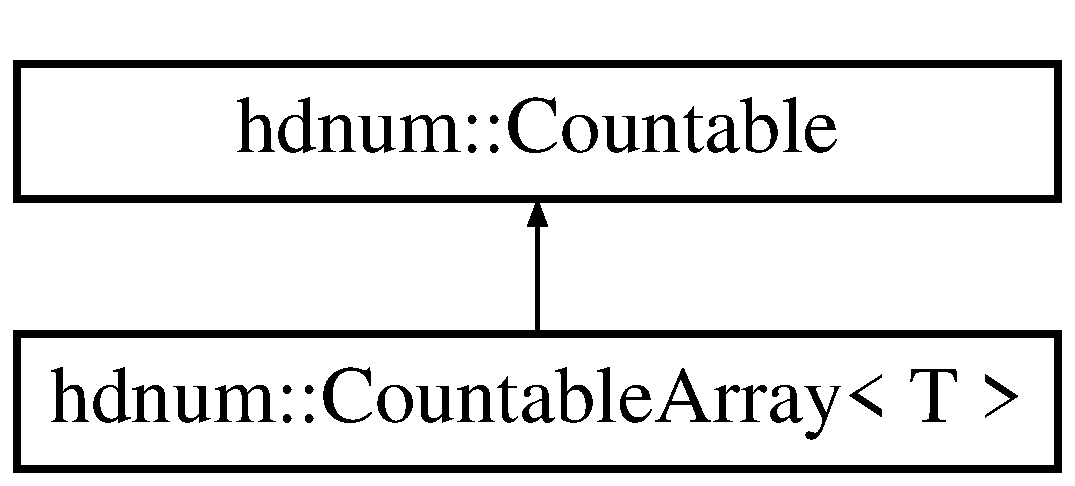
\includegraphics[height=2cm]{classhdnum_1_1Countable}
\end{center}
\end{figure}
\subsection*{Public Member Functions}
\begin{DoxyCompactItemize}
\item 
\hypertarget{classhdnum_1_1Countable_a45b6c9588aad15524d23935086829847}{
\hyperlink{classhdnum_1_1Countable_a45b6c9588aad15524d23935086829847}{Countable} ()}
\label{classhdnum_1_1Countable_a45b6c9588aad15524d23935086829847}

\begin{DoxyCompactList}\small\item\em Default constructor. \item\end{DoxyCompactList}\item 
\hypertarget{classhdnum_1_1Countable_a1bf12e6a87ae66f1b310a9c202fd9844}{
\hyperlink{classhdnum_1_1Countable_a1bf12e6a87ae66f1b310a9c202fd9844}{Countable} (const \hyperlink{classhdnum_1_1Countable}{Countable} \&)}
\label{classhdnum_1_1Countable_a1bf12e6a87ae66f1b310a9c202fd9844}

\begin{DoxyCompactList}\small\item\em copy constructor: new object, no pointer exists \item\end{DoxyCompactList}\item 
\hypertarget{classhdnum_1_1Countable_af7d443a1f3195b7b456d47f5f76f5fcf}{
\hyperlink{classhdnum_1_1Countable}{Countable} \& \hyperlink{classhdnum_1_1Countable_af7d443a1f3195b7b456d47f5f76f5fcf}{operator=} (const \hyperlink{classhdnum_1_1Countable}{Countable} \&)}
\label{classhdnum_1_1Countable_af7d443a1f3195b7b456d47f5f76f5fcf}

\begin{DoxyCompactList}\small\item\em number of pointers does not change \item\end{DoxyCompactList}\item 
\hypertarget{classhdnum_1_1Countable_aa8116fca1ddfee3971847c55f9fe15bc}{
void \hyperlink{classhdnum_1_1Countable_aa8116fca1ddfee3971847c55f9fe15bc}{reference\_\-counter\_\-increment} () const }
\label{classhdnum_1_1Countable_aa8116fca1ddfee3971847c55f9fe15bc}

\begin{DoxyCompactList}\small\item\em increment reference counter \item\end{DoxyCompactList}\item 
\hypertarget{classhdnum_1_1Countable_a02c3a28bb4d4bfc74615fb5648e250dc}{
void \hyperlink{classhdnum_1_1Countable_a02c3a28bb4d4bfc74615fb5648e250dc}{reference\_\-counter\_\-decrement} () const }
\label{classhdnum_1_1Countable_a02c3a28bb4d4bfc74615fb5648e250dc}

\begin{DoxyCompactList}\small\item\em decrement reference counter \item\end{DoxyCompactList}\item 
\hypertarget{classhdnum_1_1Countable_a13818b6671192ee672b96abaf2467eb2}{
bool \hyperlink{classhdnum_1_1Countable_a13818b6671192ee672b96abaf2467eb2}{reference\_\-counter\_\-zero} () const }
\label{classhdnum_1_1Countable_a13818b6671192ee672b96abaf2467eb2}

\begin{DoxyCompactList}\small\item\em check wether the reference counter is zero \item\end{DoxyCompactList}\item 
\hypertarget{classhdnum_1_1Countable_aae830a9bca6bf2223b1383e2c4dd7d22}{
int \hyperlink{classhdnum_1_1Countable_aae830a9bca6bf2223b1383e2c4dd7d22}{get\_\-reference\_\-counter} () const }
\label{classhdnum_1_1Countable_aae830a9bca6bf2223b1383e2c4dd7d22}

\begin{DoxyCompactList}\small\item\em get value of reference counter \item\end{DoxyCompactList}\item 
\hyperlink{classhdnum_1_1Countable_a3a8b009981f6c23579c45770ab18f1aa}{$\sim$Countable} ()
\begin{DoxyCompactList}\small\item\em Destructor. \item\end{DoxyCompactList}\end{DoxyCompactItemize}


\subsection{Detailed Description}
Base class for object pointed to by \hyperlink{classhdnum_1_1CP}{CP}. This provides the necessary functionality in the target object for the \hyperlink{classhdnum_1_1CP}{CP} template class to work. 

\subsection{Constructor \& Destructor Documentation}
\hypertarget{classhdnum_1_1Countable_a3a8b009981f6c23579c45770ab18f1aa}{
\index{hdnum::Countable@{hdnum::Countable}!$\sim$Countable@{$\sim$Countable}}
\index{$\sim$Countable@{$\sim$Countable}!hdnum::Countable@{hdnum::Countable}}
\subsubsection[{$\sim$Countable}]{\setlength{\rightskip}{0pt plus 5cm}hdnum::Countable::$\sim$Countable ()\hspace{0.3cm}{\ttfamily  \mbox{[}inline\mbox{]}}}}
\label{classhdnum_1_1Countable_a3a8b009981f6c23579c45770ab18f1aa}


Destructor. 

Warn if any \hyperlink{classhdnum_1_1CP}{CP} is still pointing to us. 

The documentation for this class was generated from the following file:\begin{DoxyCompactItemize}
\item 
src/\hyperlink{countingptr_8hh}{countingptr.hh}\end{DoxyCompactItemize}

\hypertarget{classhdnum_1_1CountableArray}{
\section{hdnum::CountableArray$<$ T $>$ Class Template Reference}
\label{classhdnum_1_1CountableArray}\index{hdnum::CountableArray@{hdnum::CountableArray}}
}


Dynamic array that can be used with the reference counting pointer.  




{\ttfamily \#include $<$countablearray.hh$>$}

Inheritance diagram for hdnum::CountableArray$<$ T $>$:\begin{figure}[H]
\begin{center}
\leavevmode
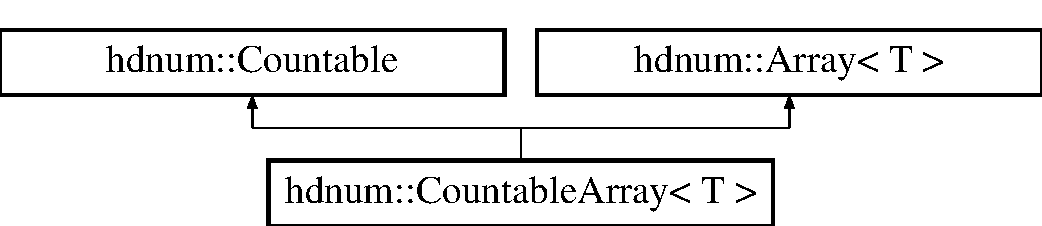
\includegraphics[height=2cm]{classhdnum_1_1CountableArray}
\end{center}
\end{figure}
\subsection*{Public Types}
\begin{DoxyCompactItemize}
\item 
\hypertarget{classhdnum_1_1CountableArray_a8505dbe8243864d347eb74d46d5c4fb7}{
typedef std::size\_\-t \hyperlink{classhdnum_1_1CountableArray_a8505dbe8243864d347eb74d46d5c4fb7}{size\_\-type}}
\label{classhdnum_1_1CountableArray_a8505dbe8243864d347eb74d46d5c4fb7}

\begin{DoxyCompactList}\small\item\em Type used for array indices. \item\end{DoxyCompactList}\end{DoxyCompactItemize}
\subsection*{Public Member Functions}
\begin{DoxyCompactItemize}
\item 
\hypertarget{classhdnum_1_1CountableArray_afb98f6c0294a385f78f34d77b172de58}{
\hyperlink{classhdnum_1_1CountableArray_afb98f6c0294a385f78f34d77b172de58}{CountableArray} ()}
\label{classhdnum_1_1CountableArray_afb98f6c0294a385f78f34d77b172de58}

\begin{DoxyCompactList}\small\item\em make empty array \item\end{DoxyCompactList}\item 
\hypertarget{classhdnum_1_1CountableArray_a4e0bc82910abedec2a59fb7c2dabf7f3}{
\hyperlink{classhdnum_1_1CountableArray_a4e0bc82910abedec2a59fb7c2dabf7f3}{CountableArray} (\hyperlink{classhdnum_1_1CountableArray_a8505dbe8243864d347eb74d46d5c4fb7}{size\_\-type} \_\-n)}
\label{classhdnum_1_1CountableArray_a4e0bc82910abedec2a59fb7c2dabf7f3}

\begin{DoxyCompactList}\small\item\em make array with \_\-n uninitialized components \item\end{DoxyCompactList}\item 
\hypertarget{classhdnum_1_1CountableArray_a19cb42db927a26a18c19600f7b1b9bc1}{
\hyperlink{classhdnum_1_1CountableArray_a19cb42db927a26a18c19600f7b1b9bc1}{CountableArray} (\hyperlink{classhdnum_1_1CountableArray_a8505dbe8243864d347eb74d46d5c4fb7}{size\_\-type} \_\-n, const T \&\_\-t)}
\label{classhdnum_1_1CountableArray_a19cb42db927a26a18c19600f7b1b9bc1}

\begin{DoxyCompactList}\small\item\em make array with \_\-n initialized components \item\end{DoxyCompactList}\end{DoxyCompactItemize}


\subsection{Detailed Description}
\subsubsection*{template$<$class T$>$ class hdnum::CountableArray$<$ T $>$}

Dynamic array that can be used with the reference counting pointer. Provides a dyamically allocated array with access operator, resizing and size method. 

The documentation for this class was generated from the following file:\begin{DoxyCompactItemize}
\item 
src/\hyperlink{countablearray_8hh}{countablearray.hh}\end{DoxyCompactItemize}

\hypertarget{classhdnum_1_1CountableException}{
\section{hdnum::CountableException Class Reference}
\label{classhdnum_1_1CountableException}\index{hdnum::CountableException@{hdnum::CountableException}}
}
\subsection*{Public Member Functions}
\begin{DoxyCompactItemize}
\item 
\hypertarget{classhdnum_1_1CountableException_aed359e1ef23bda6894f557148665102f}{
{\bfseries CountableException} (int i)}
\label{classhdnum_1_1CountableException_aed359e1ef23bda6894f557148665102f}

\item 
\hypertarget{classhdnum_1_1CountableException_a91e950ea5654bd37cc37dea6b75cbb3c}{
int {\bfseries get\_\-counter} () const }
\label{classhdnum_1_1CountableException_a91e950ea5654bd37cc37dea6b75cbb3c}

\end{DoxyCompactItemize}


The documentation for this class was generated from the following file:\begin{DoxyCompactItemize}
\item 
src/\hyperlink{countingptr_8hh}{countingptr.hh}\end{DoxyCompactItemize}

\hypertarget{classhdnum_1_1CP}{
\section{hdnum::CP$<$ T, P $>$ Class Template Reference}
\label{classhdnum_1_1CP}\index{hdnum::CP@{hdnum::CP}}
}


Pointer with a reference count in the pointed-\/to object.  




{\ttfamily \#include $<$countingptr.hh$>$}

\subsection*{Public Member Functions}
\begin{DoxyCompactItemize}
\item 
\hypertarget{classhdnum_1_1CP_a44d2479eb8eaa687b88dfc8cb7910cf2}{
\hyperlink{classhdnum_1_1CP_a44d2479eb8eaa687b88dfc8cb7910cf2}{CP} ()}
\label{classhdnum_1_1CP_a44d2479eb8eaa687b88dfc8cb7910cf2}

\begin{DoxyCompactList}\small\item\em Construct a \hyperlink{classhdnum_1_1CP}{CP} object which points to 0. \item\end{DoxyCompactList}\item 
\hypertarget{classhdnum_1_1CP_a12f46cf7a0c9e58b2ac7d2e33687e5af}{
\hyperlink{classhdnum_1_1CP_a12f46cf7a0c9e58b2ac7d2e33687e5af}{CP} (T $\ast$p\_\-)}
\label{classhdnum_1_1CP_a12f46cf7a0c9e58b2ac7d2e33687e5af}

\begin{DoxyCompactList}\small\item\em Construct a \hyperlink{classhdnum_1_1CP}{CP} object which points to p\_\- (which may be 0). \item\end{DoxyCompactList}\item 
\hypertarget{classhdnum_1_1CP_a61b2d8e087ef4075862c638d1c2794d5}{
\hyperlink{classhdnum_1_1CP_a61b2d8e087ef4075862c638d1c2794d5}{CP} (const \hyperlink{classhdnum_1_1CP}{CP}$<$ T $>$ \&cp)}
\label{classhdnum_1_1CP_a61b2d8e087ef4075862c638d1c2794d5}

\begin{DoxyCompactList}\small\item\em Copy constructor. \item\end{DoxyCompactList}\item 
\hypertarget{classhdnum_1_1CP_a9054453462ece1b56e0c9c94335f0aff}{
\hyperlink{classhdnum_1_1CP_a9054453462ece1b56e0c9c94335f0aff}{$\sim$CP} ()}
\label{classhdnum_1_1CP_a9054453462ece1b56e0c9c94335f0aff}

\begin{DoxyCompactList}\small\item\em Destructor. \item\end{DoxyCompactList}\item 
\hypertarget{classhdnum_1_1CP_acadabf2279d172f35acb2a7d2f708776}{
\hyperlink{classhdnum_1_1CP}{CP}$<$ T $>$ \& \hyperlink{classhdnum_1_1CP_acadabf2279d172f35acb2a7d2f708776}{operator=} (T $\ast$p\_\-)}
\label{classhdnum_1_1CP_acadabf2279d172f35acb2a7d2f708776}

\begin{DoxyCompactList}\small\item\em assignment from a C pointer \item\end{DoxyCompactList}\item 
\hypertarget{classhdnum_1_1CP_ae98fff24e4e6e981f86f04aa2241324a}{
\hyperlink{classhdnum_1_1CP}{CP}$<$ T $>$ \& \hyperlink{classhdnum_1_1CP_ae98fff24e4e6e981f86f04aa2241324a}{operator=} (const \hyperlink{classhdnum_1_1CP}{CP}$<$ T $>$ \&cp)}
\label{classhdnum_1_1CP_ae98fff24e4e6e981f86f04aa2241324a}

\begin{DoxyCompactList}\small\item\em copy operator \item\end{DoxyCompactList}\item 
\hypertarget{classhdnum_1_1CP_a2b24f8dfb8382e01a16a17ae4d65c68f}{
T $\ast$ \hyperlink{classhdnum_1_1CP_a2b24f8dfb8382e01a16a17ae4d65c68f}{operator-\/$>$} () const }
\label{classhdnum_1_1CP_a2b24f8dfb8382e01a16a17ae4d65c68f}

\begin{DoxyCompactList}\small\item\em target element access \item\end{DoxyCompactList}\item 
\hypertarget{classhdnum_1_1CP_a923fbd611e128b2c45edd3f6d2ff9326}{
T \& \hyperlink{classhdnum_1_1CP_a923fbd611e128b2c45edd3f6d2ff9326}{operator$\ast$} () const }
\label{classhdnum_1_1CP_a923fbd611e128b2c45edd3f6d2ff9326}

\begin{DoxyCompactList}\small\item\em dereference operator \item\end{DoxyCompactList}\item 
\hypertarget{classhdnum_1_1CP_a9d8b201344b1cf82d1e9b1012efdff8f}{
bool \hyperlink{classhdnum_1_1CP_a9d8b201344b1cf82d1e9b1012efdff8f}{operator==} (const \hyperlink{classhdnum_1_1CP}{CP}$<$ T $>$ \&cp) const }
\label{classhdnum_1_1CP_a9d8b201344b1cf82d1e9b1012efdff8f}

\begin{DoxyCompactList}\small\item\em check whether both point to same target \item\end{DoxyCompactList}\item 
\hypertarget{classhdnum_1_1CP_ac27eb29e95f1008def9303b31a2e0822}{
bool \hyperlink{classhdnum_1_1CP_ac27eb29e95f1008def9303b31a2e0822}{operator!=} (const \hyperlink{classhdnum_1_1CP}{CP}$<$ T $>$ \&cp) const }
\label{classhdnum_1_1CP_ac27eb29e95f1008def9303b31a2e0822}

\begin{DoxyCompactList}\small\item\em check whether target have different adress \item\end{DoxyCompactList}\end{DoxyCompactItemize}


\subsection{Detailed Description}
\subsubsection*{template$<$typename T, typename P = DeletingMemoryManagementPolicy$>$ class hdnum::CP$<$ T, P $>$}

Pointer with a reference count in the pointed-\/to object. 
\begin{DoxyTemplParams}{Template Parameters}
\item[{\em T}]The type of the pointed-\/to object. Must be derived from \hyperlink{classhdnum_1_1Countable}{Countable}. \item[{\em P}]What to do when the reference count reaches 0. Two predefined policy classes are available: \hyperlink{classhdnum_1_1NondeletingMemoryManagementPolicy}{NondeletingMemoryManagementPolicy} and \hyperlink{classhdnum_1_1DeletingMemoryManagementPolicy}{DeletingMemoryManagementPolicy} (the default).\end{DoxyTemplParams}
An object cp of class \hyperlink{classhdnum_1_1CP}{CP} points to another object of a class derived from \hyperlink{classhdnum_1_1Countable}{Countable}, or to 0. If it does not point to 0, it will keep track of how many \hyperlink{classhdnum_1_1CP}{CP} objects point to the same object. If cp stops pointing to the target object, it will decrement its reference count, and if the reference count reaches zero may or may not delete the target object, depending on what the memory managment policy dictates.

cp may be set via assingment from an apropriate C pointer or another \hyperlink{classhdnum_1_1CP}{CP} of the same type. To access the pointed to object, the expressions $\ast$cp and cp-\/$>$member may be used, where member is a member of the pointed to object. Finally, \hyperlink{classhdnum_1_1CP}{CP} objects may be compared using == and != to find out whether they point to the same object. 

The documentation for this class was generated from the following file:\begin{DoxyCompactItemize}
\item 
src/\hyperlink{countingptr_8hh}{countingptr.hh}\end{DoxyCompactItemize}

\hypertarget{classhdnum_1_1DeletingMemoryManagementPolicy}{
\section{hdnum::DeletingMemoryManagementPolicy Class Reference}
\label{classhdnum_1_1DeletingMemoryManagementPolicy}\index{hdnum::DeletingMemoryManagementPolicy@{hdnum::DeletingMemoryManagementPolicy}}
}


Delete target if reference count reaches zero.  




{\ttfamily \#include $<$countingptr.hh$>$}

\subsection*{Static Public Member Functions}
\begin{DoxyCompactItemize}
\item 
\hypertarget{classhdnum_1_1DeletingMemoryManagementPolicy_a39e3349b6f0e03ecf992f31f9da9ccb9}{
{\footnotesize template$<$typename T $>$ }\\static void {\bfseries delete\_\-action} (T $\ast$p)}
\label{classhdnum_1_1DeletingMemoryManagementPolicy_a39e3349b6f0e03ecf992f31f9da9ccb9}

\end{DoxyCompactItemize}


\subsection{Detailed Description}
Delete target if reference count reaches zero. If this class is given to \hyperlink{classhdnum_1_1CP}{CP} as the memory management policy, the \hyperlink{classhdnum_1_1CP}{CP} objects will delete the pointed to object if the reference count reaches zero. 

The documentation for this class was generated from the following file:\begin{DoxyCompactItemize}
\item 
src/\hyperlink{countingptr_8hh}{countingptr.hh}\end{DoxyCompactItemize}

\hypertarget{classhdnum_1_1DenseMatrix}{
\section{hdnum::DenseMatrix$<$ REAL $>$ Class Template Reference}
\label{classhdnum_1_1DenseMatrix}\index{hdnum::DenseMatrix@{hdnum::DenseMatrix}}
}


Class with mathematical matrix operations.  




{\ttfamily \#include $<$densematrix.hh$>$}

\subsection*{Public Types}
\begin{DoxyCompactItemize}
\item 
\hypertarget{classhdnum_1_1DenseMatrix_ac524278e2ff8ab9e47d03376bb1d35cc}{
typedef std::size\_\-t \hyperlink{classhdnum_1_1DenseMatrix_ac524278e2ff8ab9e47d03376bb1d35cc}{size\_\-type}}
\label{classhdnum_1_1DenseMatrix_ac524278e2ff8ab9e47d03376bb1d35cc}

\begin{DoxyCompactList}\small\item\em Type used for array indices. \item\end{DoxyCompactList}\item 
\hypertarget{classhdnum_1_1DenseMatrix_a74403a826f8e6d873e0108e3dfc0b271}{
typedef std::vector$<$ REAL $>$ {\bfseries VType}}
\label{classhdnum_1_1DenseMatrix_a74403a826f8e6d873e0108e3dfc0b271}

\item 
\hypertarget{classhdnum_1_1DenseMatrix_ab680a3c46c7cba92a82eef5d4d3eb0b9}{
typedef VType::const\_\-iterator {\bfseries ConstVectorIterator}}
\label{classhdnum_1_1DenseMatrix_ab680a3c46c7cba92a82eef5d4d3eb0b9}

\item 
\hypertarget{classhdnum_1_1DenseMatrix_ac5d21573d755db58b7a53bd49b2e89d3}{
typedef VType::iterator {\bfseries VectorIterator}}
\label{classhdnum_1_1DenseMatrix_ac5d21573d755db58b7a53bd49b2e89d3}

\end{DoxyCompactItemize}
\subsection*{Public Member Functions}
\begin{DoxyCompactItemize}
\item 
\hypertarget{classhdnum_1_1DenseMatrix_aa8aebe927f62a0f8f9728225cbdf8f82}{
{\bfseries DenseMatrix} (const std::size\_\-t \_\-rows, const std::size\_\-t \_\-cols, const REAL def\_\-val=0)}
\label{classhdnum_1_1DenseMatrix_aa8aebe927f62a0f8f9728225cbdf8f82}

\item 
\hypertarget{classhdnum_1_1DenseMatrix_a628d1da6da24e801560d14d8b7c672a4}{
void {\bfseries addNewRow} (const \hyperlink{classhdnum_1_1Vector}{hdnum::Vector}$<$ REAL $>$ \&rowvector)}
\label{classhdnum_1_1DenseMatrix_a628d1da6da24e801560d14d8b7c672a4}

\item 
size\_\-t \hyperlink{classhdnum_1_1DenseMatrix_aa5cc4ed9e7ccaafa1d9396ded5e7189b}{rowsize} () const 
\begin{DoxyCompactList}\small\item\em get number of rows of the matrix \item\end{DoxyCompactList}\item 
size\_\-t \hyperlink{classhdnum_1_1DenseMatrix_ac120c9c3beacb257ea9a8596079bfe4c}{colsize} () const 
\begin{DoxyCompactList}\small\item\em get number of columns of the matrix \item\end{DoxyCompactList}\item 
\hypertarget{classhdnum_1_1DenseMatrix_ac3efbe4dfe52f76b40a83be56ccfe13a}{
bool {\bfseries scientific} () const }
\label{classhdnum_1_1DenseMatrix_ac3efbe4dfe52f76b40a83be56ccfe13a}

\item 
void \hyperlink{classhdnum_1_1DenseMatrix_afef39f0ff9f8ade07b226172b425fb2f}{scientific} (bool b) const 
\begin{DoxyCompactList}\small\item\em Switch between floating point (default=true) and fixed point (false) display. \item\end{DoxyCompactList}\item 
\hypertarget{classhdnum_1_1DenseMatrix_a569e06e19a7f8789677bda6c80b62a79}{
std::size\_\-t \hyperlink{classhdnum_1_1DenseMatrix_a569e06e19a7f8789677bda6c80b62a79}{iwidth} () const }
\label{classhdnum_1_1DenseMatrix_a569e06e19a7f8789677bda6c80b62a79}

\begin{DoxyCompactList}\small\item\em get index field width for pretty-\/printing \item\end{DoxyCompactList}\item 
\hypertarget{classhdnum_1_1DenseMatrix_a7fb556886e5de7700f5eaf8b855414c7}{
std::size\_\-t \hyperlink{classhdnum_1_1DenseMatrix_a7fb556886e5de7700f5eaf8b855414c7}{width} () const }
\label{classhdnum_1_1DenseMatrix_a7fb556886e5de7700f5eaf8b855414c7}

\begin{DoxyCompactList}\small\item\em get data field width for pretty-\/printing \item\end{DoxyCompactList}\item 
\hypertarget{classhdnum_1_1DenseMatrix_a289a6535cdeda96e7054e8fdecde8a49}{
std::size\_\-t \hyperlink{classhdnum_1_1DenseMatrix_a289a6535cdeda96e7054e8fdecde8a49}{precision} () const }
\label{classhdnum_1_1DenseMatrix_a289a6535cdeda96e7054e8fdecde8a49}

\begin{DoxyCompactList}\small\item\em get data precision for pretty-\/printing \item\end{DoxyCompactList}\item 
\hypertarget{classhdnum_1_1DenseMatrix_a9d3daebcef6d176c9300a4ce6d7691ad}{
void \hyperlink{classhdnum_1_1DenseMatrix_a9d3daebcef6d176c9300a4ce6d7691ad}{iwidth} (std::size\_\-t i) const }
\label{classhdnum_1_1DenseMatrix_a9d3daebcef6d176c9300a4ce6d7691ad}

\begin{DoxyCompactList}\small\item\em set index field width for pretty-\/printing \item\end{DoxyCompactList}\item 
\hypertarget{classhdnum_1_1DenseMatrix_a58fe239565e09a1e31539d83241ac5cd}{
void \hyperlink{classhdnum_1_1DenseMatrix_a58fe239565e09a1e31539d83241ac5cd}{width} (std::size\_\-t i) const }
\label{classhdnum_1_1DenseMatrix_a58fe239565e09a1e31539d83241ac5cd}

\begin{DoxyCompactList}\small\item\em set data field width for pretty-\/printing \item\end{DoxyCompactList}\item 
\hypertarget{classhdnum_1_1DenseMatrix_a7c685b80c0fce12bf1b93ae788acdb91}{
void \hyperlink{classhdnum_1_1DenseMatrix_a7c685b80c0fce12bf1b93ae788acdb91}{precision} (std::size\_\-t i) const }
\label{classhdnum_1_1DenseMatrix_a7c685b80c0fce12bf1b93ae788acdb91}

\begin{DoxyCompactList}\small\item\em set data precision for pretty-\/printing \item\end{DoxyCompactList}\item 
REAL \& \hyperlink{classhdnum_1_1DenseMatrix_aaaedd0bde6bff8e04a0df7ef2afccbf5}{operator()} (const std::size\_\-t row, const std::size\_\-t col)
\begin{DoxyCompactList}\small\item\em (i,j)-\/operator for accessing entries of a (m x n)-\/matrix directly \item\end{DoxyCompactList}\item 
\hypertarget{classhdnum_1_1DenseMatrix_ab7c954af7b135112fa5f729dbac12180}{
const REAL \& {\bfseries operator()} (const std::size\_\-t row, const std::size\_\-t col) const }
\label{classhdnum_1_1DenseMatrix_ab7c954af7b135112fa5f729dbac12180}

\item 
\hypertarget{classhdnum_1_1DenseMatrix_a707394b6c91149af1b9c8d58d2936c54}{
const ConstVectorIterator {\bfseries operator\mbox{[}$\,$\mbox{]}} (const std::size\_\-t row) const }
\label{classhdnum_1_1DenseMatrix_a707394b6c91149af1b9c8d58d2936c54}

\item 
VectorIterator \hyperlink{classhdnum_1_1DenseMatrix_a0b75e9b18cb4ef4eea002473d889bff8}{operator\mbox{[}$\,$\mbox{]}} (const std::size\_\-t row)
\begin{DoxyCompactList}\small\item\em \mbox{[}i\mbox{]}\mbox{[}j\mbox{]}-\/operator for accessing entries of a (m x n)-\/matrix directly \item\end{DoxyCompactList}\item 
\hyperlink{classhdnum_1_1DenseMatrix}{DenseMatrix} \& \hyperlink{classhdnum_1_1DenseMatrix_a45a853bb1f130f7eed4590246b2b5cb5}{operator=} (const \hyperlink{classhdnum_1_1DenseMatrix}{DenseMatrix} \&A)
\begin{DoxyCompactList}\small\item\em assignment operator \item\end{DoxyCompactList}\item 
\hyperlink{classhdnum_1_1DenseMatrix}{DenseMatrix} \& \hyperlink{classhdnum_1_1DenseMatrix_a71db0fae467cdc4951ae4f3c67165b2f}{operator=} (const REAL value)
\begin{DoxyCompactList}\small\item\em assignment from a scalar value \item\end{DoxyCompactList}\item 
\hyperlink{classhdnum_1_1DenseMatrix}{DenseMatrix} \& \hyperlink{classhdnum_1_1DenseMatrix_aebf9d5238390cc39144b8eeb2d76a6f0}{operator+=} (const \hyperlink{classhdnum_1_1DenseMatrix}{DenseMatrix} \&B)
\begin{DoxyCompactList}\small\item\em Addition assignment. \item\end{DoxyCompactList}\item 
\hyperlink{classhdnum_1_1DenseMatrix}{DenseMatrix} \& \hyperlink{classhdnum_1_1DenseMatrix_a4b0031fef6e91b5f319862f16457ac9f}{operator-\/=} (const \hyperlink{classhdnum_1_1DenseMatrix}{DenseMatrix} \&B)
\begin{DoxyCompactList}\small\item\em Subtraction assignment. \item\end{DoxyCompactList}\item 
\hyperlink{classhdnum_1_1DenseMatrix}{DenseMatrix} \& \hyperlink{classhdnum_1_1DenseMatrix_a0681152377c82cc1bffa0384577e3d6b}{operator$\ast$=} (const REAL s)
\begin{DoxyCompactList}\small\item\em Scalar multiplication assignment. \item\end{DoxyCompactList}\item 
\hyperlink{classhdnum_1_1DenseMatrix}{DenseMatrix} \& \hyperlink{classhdnum_1_1DenseMatrix_a05fab8204f026598d4d97a04013ed7c5}{operator/=} (const REAL s)
\begin{DoxyCompactList}\small\item\em Scalar division assignment. \item\end{DoxyCompactList}\item 
void \hyperlink{classhdnum_1_1DenseMatrix_a60a10bbc94192242d3206df18eb0978b}{update} (const REAL s, const \hyperlink{classhdnum_1_1DenseMatrix}{DenseMatrix} \&B)
\begin{DoxyCompactList}\small\item\em Scaled update of a \hyperlink{classhdnum_1_1Matrix}{Matrix}. \item\end{DoxyCompactList}\item 
{\footnotesize template$<$class V $>$ }\\void \hyperlink{classhdnum_1_1DenseMatrix_a63a0aa62c65545ae7aeee7a44e10568e}{mv} (\hyperlink{classhdnum_1_1Vector}{Vector}$<$ V $>$ \&y, const \hyperlink{classhdnum_1_1Vector}{Vector}$<$ V $>$ \&x) const 
\begin{DoxyCompactList}\small\item\em matrix vector product y = A$\ast$x \item\end{DoxyCompactList}\item 
{\footnotesize template$<$class V $>$ }\\void \hyperlink{classhdnum_1_1DenseMatrix_a7c179eb4b54a828bf8624f3222f710ce}{umv} (\hyperlink{classhdnum_1_1Vector}{Vector}$<$ V $>$ \&y, const \hyperlink{classhdnum_1_1Vector}{Vector}$<$ V $>$ \&x) const 
\begin{DoxyCompactList}\small\item\em update matrix vector product y += A$\ast$x \item\end{DoxyCompactList}\item 
{\footnotesize template$<$class V $>$ }\\void \hyperlink{classhdnum_1_1DenseMatrix_aabf780a319d2d9d4379f8d5832c1a99c}{umv} (\hyperlink{classhdnum_1_1Vector}{Vector}$<$ V $>$ \&y, const V \&s, const \hyperlink{classhdnum_1_1Vector}{Vector}$<$ V $>$ \&x) const 
\begin{DoxyCompactList}\small\item\em update matrix vector product y += sA$\ast$x \item\end{DoxyCompactList}\item 
void \hyperlink{classhdnum_1_1DenseMatrix_ad79f3e02f3a7a3b2639992cc717470d9}{mm} (const \hyperlink{classhdnum_1_1DenseMatrix}{DenseMatrix}$<$ REAL $>$ \&A, const \hyperlink{classhdnum_1_1DenseMatrix}{DenseMatrix}$<$ REAL $>$ \&B)
\begin{DoxyCompactList}\small\item\em assign to matrix product C = A$\ast$B to matrix C \item\end{DoxyCompactList}\item 
void \hyperlink{classhdnum_1_1DenseMatrix_a45630f26522adf719f3947d09145b7c2}{umm} (const \hyperlink{classhdnum_1_1DenseMatrix}{DenseMatrix}$<$ REAL $>$ \&A, const \hyperlink{classhdnum_1_1DenseMatrix}{DenseMatrix}$<$ REAL $>$ \&B)
\begin{DoxyCompactList}\small\item\em add matrix product A$\ast$B to matrix C \item\end{DoxyCompactList}\item 
void \hyperlink{classhdnum_1_1DenseMatrix_a815aef5dfc09aecd12472dbfd4ab1e37}{sc} (const \hyperlink{classhdnum_1_1Vector}{Vector}$<$ REAL $>$ \&x, std::size\_\-t k)
\begin{DoxyCompactList}\small\item\em set column: make x the k'th column of A \item\end{DoxyCompactList}\item 
void \hyperlink{classhdnum_1_1DenseMatrix_a833f6bd37078251cb91018a7c0c339aa}{sr} (const \hyperlink{classhdnum_1_1Vector}{Vector}$<$ REAL $>$ \&x, std::size\_\-t k)
\begin{DoxyCompactList}\small\item\em set row: make x the k'th row of A \item\end{DoxyCompactList}\item 
\hypertarget{classhdnum_1_1DenseMatrix_aea0ca5908d85d37f61646088e7623159}{
REAL \hyperlink{classhdnum_1_1DenseMatrix_aea0ca5908d85d37f61646088e7623159}{norm\_\-infty} () const }
\label{classhdnum_1_1DenseMatrix_aea0ca5908d85d37f61646088e7623159}

\begin{DoxyCompactList}\small\item\em compute row sum norm \item\end{DoxyCompactList}\item 
\hypertarget{classhdnum_1_1DenseMatrix_abff8476e13341659ce2fcb6145dd351b}{
REAL \hyperlink{classhdnum_1_1DenseMatrix_abff8476e13341659ce2fcb6145dd351b}{norm\_\-1} () const }
\label{classhdnum_1_1DenseMatrix_abff8476e13341659ce2fcb6145dd351b}

\begin{DoxyCompactList}\small\item\em compute column sum norm \item\end{DoxyCompactList}\item 
\hyperlink{classhdnum_1_1Vector}{Vector}$<$ REAL $>$ \hyperlink{classhdnum_1_1DenseMatrix_a6c43e793e3c9d91b1c216137a26f9ab7}{operator$\ast$} (const \hyperlink{classhdnum_1_1Vector}{Vector}$<$ REAL $>$ \&x)
\begin{DoxyCompactList}\small\item\em vector = matrix $\ast$ vector \item\end{DoxyCompactList}\item 
\hyperlink{classhdnum_1_1DenseMatrix}{DenseMatrix} \hyperlink{classhdnum_1_1DenseMatrix_a32bf5f7e4113e65aaeee04177d22a522}{operator$\ast$} (const \hyperlink{classhdnum_1_1DenseMatrix}{DenseMatrix} \&x) const 
\begin{DoxyCompactList}\small\item\em matrix = matrix $\ast$ matrix \item\end{DoxyCompactList}\item 
\hyperlink{classhdnum_1_1DenseMatrix}{DenseMatrix} \hyperlink{classhdnum_1_1DenseMatrix_ab31d1c60b8078d01bd131e36a486f091}{operator+} (const \hyperlink{classhdnum_1_1DenseMatrix}{DenseMatrix} \&x) const 
\begin{DoxyCompactList}\small\item\em matrix = matrix + matrix \item\end{DoxyCompactList}\item 
\hyperlink{classhdnum_1_1DenseMatrix}{DenseMatrix} \hyperlink{classhdnum_1_1DenseMatrix_a0579e65186e9f546b40d718ec7502afd}{operator-\/} (const \hyperlink{classhdnum_1_1DenseMatrix}{DenseMatrix} \&x) const 
\begin{DoxyCompactList}\small\item\em matrix = matrix -\/ matrix \item\end{DoxyCompactList}\end{DoxyCompactItemize}
\subsection*{Related Functions}
(Note that these are not member functions.) \begin{DoxyCompactItemize}
\item 
{\footnotesize template$<$class T $>$ }\\void \hyperlink{classhdnum_1_1DenseMatrix_a7827fbef0d569f0b605a6a260e1571f3}{identity} (\hyperlink{classhdnum_1_1DenseMatrix}{DenseMatrix}$<$ T $>$ \&A)
\item 
{\footnotesize template$<$typename REAL $>$ }\\void \hyperlink{classhdnum_1_1DenseMatrix_a2a328e8b5dca944a17fce76e1a51c7ae}{spd} (\hyperlink{classhdnum_1_1DenseMatrix}{DenseMatrix}$<$ REAL $>$ \&A)
\item 
{\footnotesize template$<$typename REAL $>$ }\\void \hyperlink{classhdnum_1_1DenseMatrix_a1ed8c7d92b4b38e3e48eaf3a8cce1d27}{vandermonde} (\hyperlink{classhdnum_1_1DenseMatrix}{DenseMatrix}$<$ REAL $>$ \&A, const \hyperlink{classhdnum_1_1Vector}{Vector}$<$ REAL $>$ x)
\item 
{\footnotesize template$<$typename REAL $>$ }\\void \hyperlink{classhdnum_1_1DenseMatrix_a5c106d0beabd399734dd2b1a6637626e}{readMatrixFromFile} (const std::string \&filename, \hyperlink{classhdnum_1_1DenseMatrix}{DenseMatrix}$<$ REAL $>$ \&A)
\begin{DoxyCompactList}\small\item\em Read matrix from a text file. \item\end{DoxyCompactList}\end{DoxyCompactItemize}


\subsection{Detailed Description}
\subsubsection*{template$<$typename REAL$>$ class hdnum::DenseMatrix$<$ REAL $>$}

Class with mathematical matrix operations. 

\subsection{Member Function Documentation}
\hypertarget{classhdnum_1_1DenseMatrix_ac120c9c3beacb257ea9a8596079bfe4c}{
\index{hdnum::DenseMatrix@{hdnum::DenseMatrix}!colsize@{colsize}}
\index{colsize@{colsize}!hdnum::DenseMatrix@{hdnum::DenseMatrix}}
\subsubsection[{colsize}]{\setlength{\rightskip}{0pt plus 5cm}template$<$typename REAL $>$ size\_\-t {\bf hdnum::DenseMatrix}$<$ REAL $>$::colsize () const\hspace{0.3cm}{\ttfamily  \mbox{[}inline\mbox{]}}}}
\label{classhdnum_1_1DenseMatrix_ac120c9c3beacb257ea9a8596079bfe4c}


get number of columns of the matrix 

{\bfseries Example:} 
\begin{DoxyCode}
  hdnum::DenseMatrix<double> A(4,5);
  size_t nColumns = A.colsize();
  std::cout << "Matrix A has " << nColumns << " columns." << std::endl;
\end{DoxyCode}


{\bfseries Output:} \begin{DoxyVerb}
Matrix A has 5 columns.
	  \end{DoxyVerb}
 \hypertarget{classhdnum_1_1DenseMatrix_ad79f3e02f3a7a3b2639992cc717470d9}{
\index{hdnum::DenseMatrix@{hdnum::DenseMatrix}!mm@{mm}}
\index{mm@{mm}!hdnum::DenseMatrix@{hdnum::DenseMatrix}}
\subsubsection[{mm}]{\setlength{\rightskip}{0pt plus 5cm}template$<$typename REAL$>$ void {\bf hdnum::DenseMatrix}$<$ REAL $>$::mm (const {\bf DenseMatrix}$<$ REAL $>$ \& {\em A}, \/  const {\bf DenseMatrix}$<$ REAL $>$ \& {\em B})\hspace{0.3cm}{\ttfamily  \mbox{[}inline\mbox{]}}}}
\label{classhdnum_1_1DenseMatrix_ad79f3e02f3a7a3b2639992cc717470d9}


assign to matrix product C = A$\ast$B to matrix C 

Implements C = A$\ast$B where A and B are matrices


\begin{DoxyParams}{Parameters}
\item[\mbox{$\leftarrow$} {\em x}]constant reference to a \hyperlink{classhdnum_1_1DenseMatrix}{DenseMatrix} \item[\mbox{$\leftarrow$} {\em x}]constant reference to a \hyperlink{classhdnum_1_1DenseMatrix}{DenseMatrix}\end{DoxyParams}
{\bfseries Example:} 
\begin{DoxyCode}
  hdnum::DenseMatrix<double> A(2,6,1.0);
  hdnum::DenseMatrix<double> B(6,3,-1.0);

  A.scientific(false); // fixed point representation for all DenseMatrix objects
  A.width(6);          // use at least 6 columns for displaying matrix entries
  A.precision(3);      // display 3 digits behind the point 

  std::cout << "A =" << A << std::endl;
  std::cout << "B =" << B << std::endl;

  hdnum::DenseMatrix<double> C(2,3);
  C.mm(A,B);
  std::cout << "C = A*B =" << C << std::endl;
\end{DoxyCode}


{\bfseries Output:} \begin{DoxyVerb}
A =
                  0      1      2      3      4      5 
          0   1.000  1.000  1.000  1.000  1.000  1.000 
          1   1.000  1.000  1.000  1.000  1.000  1.000 

B =
                  0      1      2 
          0  -1.000 -1.000 -1.000 
          1  -1.000 -1.000 -1.000 
          2  -1.000 -1.000 -1.000 
          3  -1.000 -1.000 -1.000 
          4  -1.000 -1.000 -1.000 
          5  -1.000 -1.000 -1.000 

C = A*B =
                  0      1      2 
          0  -6.000 -6.000 -6.000 
          1  -6.000 -6.000 -6.000 
	  \end{DoxyVerb}
 \hypertarget{classhdnum_1_1DenseMatrix_a63a0aa62c65545ae7aeee7a44e10568e}{
\index{hdnum::DenseMatrix@{hdnum::DenseMatrix}!mv@{mv}}
\index{mv@{mv}!hdnum::DenseMatrix@{hdnum::DenseMatrix}}
\subsubsection[{mv}]{\setlength{\rightskip}{0pt plus 5cm}template$<$typename REAL$>$ template$<$class V $>$ void {\bf hdnum::DenseMatrix}$<$ REAL $>$::mv ({\bf Vector}$<$ V $>$ \& {\em y}, \/  const {\bf Vector}$<$ V $>$ \& {\em x}) const\hspace{0.3cm}{\ttfamily  \mbox{[}inline\mbox{]}}}}
\label{classhdnum_1_1DenseMatrix_a63a0aa62c65545ae7aeee7a44e10568e}


matrix vector product y = A$\ast$x 

Implements y = A$\ast$x where x and y are a vectors and A is a matrix


\begin{DoxyParams}{Parameters}
\item[\mbox{$\leftarrow$} {\em y}]reference to the resulting \hyperlink{classhdnum_1_1Vector}{Vector} \item[\mbox{$\leftarrow$} {\em x}]constant reference to a \hyperlink{classhdnum_1_1Vector}{Vector}\end{DoxyParams}
{\bfseries Example:} 
\begin{DoxyCode}
  hdnum::Vector<double> x(3,10.0);
  hdnum::Vector<double> y(2);
  hdnum::DenseMatrix<double> A(2,3,1.0);

  x.scientific(false); // fixed point representation for all Vector objects
  A.scientific(false); // fixed point representation for all DenseMatrix objects

  std::cout << "A =" << A << std::endl;
  std::cout << "x =" << x << std::endl;
  A.mv(y,x);
  std::cout << "y = A*x =" << y << std::endl;
\end{DoxyCode}


{\bfseries Output:} \begin{DoxyVerb}
A =
                      0          1          2 
          0       1.000      1.000      1.000 
          1       1.000      1.000      1.000 

x =
[ 0]     10.0000000
[ 1]     10.0000000
[ 2]     10.0000000

y = A*x =
[ 0]     30.0000000
[ 1]     30.0000000
	  \end{DoxyVerb}
 \hypertarget{classhdnum_1_1DenseMatrix_aaaedd0bde6bff8e04a0df7ef2afccbf5}{
\index{hdnum::DenseMatrix@{hdnum::DenseMatrix}!operator()@{operator()}}
\index{operator()@{operator()}!hdnum::DenseMatrix@{hdnum::DenseMatrix}}
\subsubsection[{operator()}]{\setlength{\rightskip}{0pt plus 5cm}template$<$typename REAL$>$ REAL\& {\bf hdnum::DenseMatrix}$<$ REAL $>$::operator() (const std::size\_\-t {\em row}, \/  const std::size\_\-t {\em col})\hspace{0.3cm}{\ttfamily  \mbox{[}inline\mbox{]}}}}
\label{classhdnum_1_1DenseMatrix_aaaedd0bde6bff8e04a0df7ef2afccbf5}


(i,j)-\/operator for accessing entries of a (m x n)-\/matrix directly 


\begin{DoxyParams}{Parameters}
\item[\mbox{$\leftarrow$} {\em i}]row index (0...m-\/1) \item[\mbox{$\leftarrow$} {\em j}]column index (0...n-\/1)\end{DoxyParams}
{\bfseries Example:} 
\begin{DoxyCode}
  hdnum::DenseMatrix<double> A(4,4);
  A.scientific(false); // fixed point representation for all DenseMatrix objects
  A.width(8);
  A.precision(3);

  identity(A);  // Defines the identity matrix of the same dimension
  std::cout << "A=" << A << std::endl;

  std::cout << "reading A(0,0)=" << A(0,0) << std::endl;

  std::cout << "resetting A(0,0) and A(2,3)..." << std::endl;
  A(0,0) = 1.234;
  A(2,3) = 432.1;
  
  std::cout << "A=" << A << std::endl;
\end{DoxyCode}


{\bfseries Output:} \begin{DoxyVerb}
A=
                    0        1        2        3 
          0     1.000    0.000    0.000    0.000 
          1     0.000    1.000    0.000    0.000 
          2     0.000    0.000    1.000    0.000 
          3     0.000    0.000    0.000    1.000 

reading A(0,0)=1.000
resetting A(0,0) and A(2,3)...
A=
                    0        1        2        3 
          0     1.234    0.000    0.000    0.000 
          1     0.000    1.000    0.000    0.000 
          2     0.000    0.000    1.000  432.100 
          3     0.000    0.000    0.000    1.000 
	  \end{DoxyVerb}
 \hypertarget{classhdnum_1_1DenseMatrix_a32bf5f7e4113e65aaeee04177d22a522}{
\index{hdnum::DenseMatrix@{hdnum::DenseMatrix}!operator$\ast$@{operator$\ast$}}
\index{operator$\ast$@{operator$\ast$}!hdnum::DenseMatrix@{hdnum::DenseMatrix}}
\subsubsection[{operator$\ast$}]{\setlength{\rightskip}{0pt plus 5cm}template$<$typename REAL$>$ {\bf DenseMatrix} {\bf hdnum::DenseMatrix}$<$ REAL $>$::operator$\ast$ (const {\bf DenseMatrix}$<$ REAL $>$ \& {\em x}) const\hspace{0.3cm}{\ttfamily  \mbox{[}inline\mbox{]}}}}
\label{classhdnum_1_1DenseMatrix_a32bf5f7e4113e65aaeee04177d22a522}


matrix = matrix $\ast$ matrix 


\begin{DoxyParams}{Parameters}
\item[\mbox{$\leftarrow$} {\em x}]constant reference to a \hyperlink{classhdnum_1_1DenseMatrix}{DenseMatrix}\end{DoxyParams}
{\bfseries Example:} 
\begin{DoxyCode}
  hdnum::DenseMatrix<double> A(3,3,2.0);
  hdnum::DenseMatrix<double> B(3,3,4.0);
  hdnum::DenseMatrix<double> C(3,3);

  A.scientific(false); // fixed point representation for all DenseMatrix objects
  A.width(8);
  A.precision(1);

  std::cout << "A=" << A << std::endl;
  std::cout << "B=" << B << std::endl;
  C=A*B;
  std::cout << "C=A*B=" << C << std::endl;
\end{DoxyCode}


{\bfseries Output:} \begin{DoxyVerb}
A=
                    0        1        2 
          0       2.0      2.0      2.0 
          1       2.0      2.0      2.0 
          2       2.0      2.0      2.0 

B=
                    0        1        2 
          0       4.0      4.0      4.0 
          1       4.0      4.0      4.0 
          2       4.0      4.0      4.0 

C=A*B=
                    0        1        2 
          0      24.0     24.0     24.0 
          1      24.0     24.0     24.0 
          2      24.0     24.0     24.0 
	  \end{DoxyVerb}
 \hypertarget{classhdnum_1_1DenseMatrix_a6c43e793e3c9d91b1c216137a26f9ab7}{
\index{hdnum::DenseMatrix@{hdnum::DenseMatrix}!operator$\ast$@{operator$\ast$}}
\index{operator$\ast$@{operator$\ast$}!hdnum::DenseMatrix@{hdnum::DenseMatrix}}
\subsubsection[{operator$\ast$}]{\setlength{\rightskip}{0pt plus 5cm}template$<$typename REAL$>$ {\bf Vector}$<$REAL$>$ {\bf hdnum::DenseMatrix}$<$ REAL $>$::operator$\ast$ (const {\bf Vector}$<$ REAL $>$ \& {\em x})\hspace{0.3cm}{\ttfamily  \mbox{[}inline\mbox{]}}}}
\label{classhdnum_1_1DenseMatrix_a6c43e793e3c9d91b1c216137a26f9ab7}


vector = matrix $\ast$ vector 


\begin{DoxyParams}{Parameters}
\item[\mbox{$\leftarrow$} {\em x}]constant reference to a \hyperlink{classhdnum_1_1Vector}{Vector}\end{DoxyParams}
{\bfseries Example:} 
\begin{DoxyCode}
  hdnum::Vector<double> x(3,4.0);
  hdnum::DenseMatrix<double> A(3,3,2.0);
  hdnum::Vector<double> y(3);

  A.scientific(false); // fixed point representation for all DenseMatrix objects
  A.width(8);
  A.precision(1);
  
  x.scientific(false); // fixed point representation for all Vector objects
  x.width(8);
  x.precision(1);


  std::cout << "A=" << A << std::endl;
  std::cout << "x=" << x << std::endl;
  y=A*x;
  std::cout << "y=A*x" << y << std::endl;
\end{DoxyCode}


{\bfseries Output:} \begin{DoxyVerb}
A=
                    0        1        2 
          0       2.0      2.0      2.0 
          1       2.0      2.0      2.0 
          2       2.0      2.0      2.0 

x=
[ 0]     4.0
[ 1]     4.0
[ 2]     4.0

y=A*x
[ 0]    24.0
[ 1]    24.0
[ 2]    24.0
	  \end{DoxyVerb}
 \hypertarget{classhdnum_1_1DenseMatrix_a0681152377c82cc1bffa0384577e3d6b}{
\index{hdnum::DenseMatrix@{hdnum::DenseMatrix}!operator$\ast$=@{operator$\ast$=}}
\index{operator$\ast$=@{operator$\ast$=}!hdnum::DenseMatrix@{hdnum::DenseMatrix}}
\subsubsection[{operator$\ast$=}]{\setlength{\rightskip}{0pt plus 5cm}template$<$typename REAL$>$ {\bf DenseMatrix}\& {\bf hdnum::DenseMatrix}$<$ REAL $>$::operator$\ast$= (const REAL {\em s})\hspace{0.3cm}{\ttfamily  \mbox{[}inline\mbox{]}}}}
\label{classhdnum_1_1DenseMatrix_a0681152377c82cc1bffa0384577e3d6b}


Scalar multiplication assignment. 

Implements A $\ast$= s where s is a scalar


\begin{DoxyParams}{Parameters}
\item[\mbox{$\leftarrow$} {\em s}]scalar value to multiply with\end{DoxyParams}
{\bfseries Example:} 
\begin{DoxyCode}
          double s = 0.5;
          hdnum::DenseMatrix<double> A(2,3,1.0);
          std::cout << "A=" << A << std::endl;
          A *= s;
          std::cout << "A=" << A << std::endl;
\end{DoxyCode}


{\bfseries Output:} \begin{DoxyVerb}
A=
                      0          1          2 
          0   1.000e+00  1.000e+00  1.000e+00 
          1   1.000e+00  1.000e+00  1.000e+00 

0.5*A =
                      0          1          2 
          0   5.000e-01  5.000e-01  5.000e-01 
          1   5.000e-01  5.000e-01  5.000e-01 
	  \end{DoxyVerb}
 \hypertarget{classhdnum_1_1DenseMatrix_ab31d1c60b8078d01bd131e36a486f091}{
\index{hdnum::DenseMatrix@{hdnum::DenseMatrix}!operator+@{operator+}}
\index{operator+@{operator+}!hdnum::DenseMatrix@{hdnum::DenseMatrix}}
\subsubsection[{operator+}]{\setlength{\rightskip}{0pt plus 5cm}template$<$typename REAL$>$ {\bf DenseMatrix} {\bf hdnum::DenseMatrix}$<$ REAL $>$::operator+ (const {\bf DenseMatrix}$<$ REAL $>$ \& {\em x}) const\hspace{0.3cm}{\ttfamily  \mbox{[}inline\mbox{]}}}}
\label{classhdnum_1_1DenseMatrix_ab31d1c60b8078d01bd131e36a486f091}


matrix = matrix + matrix 


\begin{DoxyParams}{Parameters}
\item[\mbox{$\leftarrow$} {\em x}]constant reference to a \hyperlink{classhdnum_1_1DenseMatrix}{DenseMatrix}\end{DoxyParams}
{\bfseries Example:} 
\begin{DoxyCode}
  hdnum::DenseMatrix<double> A(3,3,2.0);
  hdnum::DenseMatrix<double> B(3,3,4.0);
  hdnum::DenseMatrix<double> C(3,3);

  A.scientific(false); // fixed point representation for all DenseMatrix objects
  A.width(8);
  A.precision(1);

  std::cout << "A=" << A << std::endl;
  std::cout << "B=" << B << std::endl;
  C=A+B;
  std::cout << "C=A+B=" << C << std::endl;
\end{DoxyCode}


{\bfseries Output:} \begin{DoxyVerb}
A=
                    0        1        2 
          0       2.0      2.0      2.0 
          1       2.0      2.0      2.0 
          2       2.0      2.0      2.0 

B=
                    0        1        2 
          0       4.0      4.0      4.0 
          1       4.0      4.0      4.0 
          2       4.0      4.0      4.0 

C=A+B=
                    0        1        2 
          0       6.0      6.0      6.0 
          1       6.0      6.0      6.0 
          2       6.0      6.0      6.0 
	  \end{DoxyVerb}
 \hypertarget{classhdnum_1_1DenseMatrix_aebf9d5238390cc39144b8eeb2d76a6f0}{
\index{hdnum::DenseMatrix@{hdnum::DenseMatrix}!operator+=@{operator+=}}
\index{operator+=@{operator+=}!hdnum::DenseMatrix@{hdnum::DenseMatrix}}
\subsubsection[{operator+=}]{\setlength{\rightskip}{0pt plus 5cm}template$<$typename REAL$>$ {\bf DenseMatrix}\& {\bf hdnum::DenseMatrix}$<$ REAL $>$::operator+= (const {\bf DenseMatrix}$<$ REAL $>$ \& {\em B})\hspace{0.3cm}{\ttfamily  \mbox{[}inline\mbox{]}}}}
\label{classhdnum_1_1DenseMatrix_aebf9d5238390cc39144b8eeb2d76a6f0}


Addition assignment. 

Implements A += B matrix addition


\begin{DoxyParams}{Parameters}
\item[\mbox{$\leftarrow$} {\em B}]another \hyperlink{classhdnum_1_1Matrix}{Matrix} \end{DoxyParams}
\hypertarget{classhdnum_1_1DenseMatrix_a0579e65186e9f546b40d718ec7502afd}{
\index{hdnum::DenseMatrix@{hdnum::DenseMatrix}!operator-\/@{operator-\/}}
\index{operator-\/@{operator-\/}!hdnum::DenseMatrix@{hdnum::DenseMatrix}}
\subsubsection[{operator-\/}]{\setlength{\rightskip}{0pt plus 5cm}template$<$typename REAL$>$ {\bf DenseMatrix} {\bf hdnum::DenseMatrix}$<$ REAL $>$::operator-\/ (const {\bf DenseMatrix}$<$ REAL $>$ \& {\em x}) const\hspace{0.3cm}{\ttfamily  \mbox{[}inline\mbox{]}}}}
\label{classhdnum_1_1DenseMatrix_a0579e65186e9f546b40d718ec7502afd}


matrix = matrix -\/ matrix 


\begin{DoxyParams}{Parameters}
\item[\mbox{$\leftarrow$} {\em x}]constant reference to a \hyperlink{classhdnum_1_1DenseMatrix}{DenseMatrix}\end{DoxyParams}
{\bfseries Example:} 
\begin{DoxyCode}
  hdnum::DenseMatrix<double> A(3,3,2.0);
  hdnum::DenseMatrix<double> B(3,3,4.0);
  hdnum::DenseMatrix<double> C(3,3);

  A.scientific(false); // fixed point representation for all DenseMatrix objects
  A.width(8);
  A.precision(1);

  std::cout << "A=" << A << std::endl;
  std::cout << "B=" << B << std::endl;
  C=A-B;
  std::cout << "C=A-B=" << C << std::endl;
\end{DoxyCode}


{\bfseries Output:} \begin{DoxyVerb}
A=
                    0        1        2 
          0       2.0      2.0      2.0 
          1       2.0      2.0      2.0 
          2       2.0      2.0      2.0 

B=
                    0        1        2 
          0       4.0      4.0      4.0 
          1       4.0      4.0      4.0 
          2       4.0      4.0      4.0 

C=A-B=
                    0        1        2 
          0      -2.0     -2.0     -2.0 
          1      -2.0     -2.0     -2.0 
          2      -2.0     -2.0     -2.0 
	  \end{DoxyVerb}
 \hypertarget{classhdnum_1_1DenseMatrix_a4b0031fef6e91b5f319862f16457ac9f}{
\index{hdnum::DenseMatrix@{hdnum::DenseMatrix}!operator-\/=@{operator-\/=}}
\index{operator-\/=@{operator-\/=}!hdnum::DenseMatrix@{hdnum::DenseMatrix}}
\subsubsection[{operator-\/=}]{\setlength{\rightskip}{0pt plus 5cm}template$<$typename REAL$>$ {\bf DenseMatrix}\& {\bf hdnum::DenseMatrix}$<$ REAL $>$::operator-\/= (const {\bf DenseMatrix}$<$ REAL $>$ \& {\em B})\hspace{0.3cm}{\ttfamily  \mbox{[}inline\mbox{]}}}}
\label{classhdnum_1_1DenseMatrix_a4b0031fef6e91b5f319862f16457ac9f}


Subtraction assignment. 

Implements A -\/= B matrix subtraction


\begin{DoxyParams}{Parameters}
\item[\mbox{$\leftarrow$} {\em B}]another matrix \end{DoxyParams}
\hypertarget{classhdnum_1_1DenseMatrix_a05fab8204f026598d4d97a04013ed7c5}{
\index{hdnum::DenseMatrix@{hdnum::DenseMatrix}!operator/=@{operator/=}}
\index{operator/=@{operator/=}!hdnum::DenseMatrix@{hdnum::DenseMatrix}}
\subsubsection[{operator/=}]{\setlength{\rightskip}{0pt plus 5cm}template$<$typename REAL$>$ {\bf DenseMatrix}\& {\bf hdnum::DenseMatrix}$<$ REAL $>$::operator/= (const REAL {\em s})\hspace{0.3cm}{\ttfamily  \mbox{[}inline\mbox{]}}}}
\label{classhdnum_1_1DenseMatrix_a05fab8204f026598d4d97a04013ed7c5}


Scalar division assignment. 

Implements A /= s where s is a scalar


\begin{DoxyParams}{Parameters}
\item[\mbox{$\leftarrow$} {\em s}]scalar value to multiply with\end{DoxyParams}
{\bfseries Example:} 
\begin{DoxyCode}
          double s = 0.5;
          hdnum::DenseMatrix<double> A(2,3,1.0);
          std::cout << "A=" << A << std::endl;
          A /= s;
          std::cout << "A=" << A << std::endl;
\end{DoxyCode}


{\bfseries Output:} \begin{DoxyVerb}
A=
                      0          1          2 
          0   1.000e+00  1.000e+00  1.000e+00 
          1   1.000e+00  1.000e+00  1.000e+00 

A/0.5 =
                      0          1          2 
          0   2.000e+00  2.000e+00  2.000e+00 
          1   2.000e+00  2.000e+00  2.000e+00 
	  \end{DoxyVerb}
 \hypertarget{classhdnum_1_1DenseMatrix_a71db0fae467cdc4951ae4f3c67165b2f}{
\index{hdnum::DenseMatrix@{hdnum::DenseMatrix}!operator=@{operator=}}
\index{operator=@{operator=}!hdnum::DenseMatrix@{hdnum::DenseMatrix}}
\subsubsection[{operator=}]{\setlength{\rightskip}{0pt plus 5cm}template$<$typename REAL$>$ {\bf DenseMatrix}\& {\bf hdnum::DenseMatrix}$<$ REAL $>$::operator= (const REAL {\em value})\hspace{0.3cm}{\ttfamily  \mbox{[}inline\mbox{]}}}}
\label{classhdnum_1_1DenseMatrix_a71db0fae467cdc4951ae4f3c67165b2f}


assignment from a scalar value 

{\bfseries Example:} 
\begin{DoxyCode}
  hdnum::DenseMatrix<double> A(2,3);
  A = 5.432;
  A.scientific(false); // fixed point representation for all DenseMatrix objects
  A.width(8);
  A.precision(3);
  std::cout << "A=" << A << std::endl;
\end{DoxyCode}


{\bfseries Output:} \begin{DoxyVerb}
A=
                    0        1        2 
          0     5.432    5.432    5.432
          1     5.432    5.432    5.432
	  \end{DoxyVerb}
 \hypertarget{classhdnum_1_1DenseMatrix_a45a853bb1f130f7eed4590246b2b5cb5}{
\index{hdnum::DenseMatrix@{hdnum::DenseMatrix}!operator=@{operator=}}
\index{operator=@{operator=}!hdnum::DenseMatrix@{hdnum::DenseMatrix}}
\subsubsection[{operator=}]{\setlength{\rightskip}{0pt plus 5cm}template$<$typename REAL$>$ {\bf DenseMatrix}\& {\bf hdnum::DenseMatrix}$<$ REAL $>$::operator= (const {\bf DenseMatrix}$<$ REAL $>$ \& {\em A})\hspace{0.3cm}{\ttfamily  \mbox{[}inline\mbox{]}}}}
\label{classhdnum_1_1DenseMatrix_a45a853bb1f130f7eed4590246b2b5cb5}


assignment operator 

{\bfseries Example:} 
\begin{DoxyCode}
  hdnum::DenseMatrix<double> A(4,4);
  spd(A);
  hdnum::DenseMatrix<double> B(4,4);
  B = A;
  std::cout << "B=" << B << std::endl;
\end{DoxyCode}


{\bfseries Output:} \begin{DoxyVerb}
B=
                      0          1          2          3 
          0   4.000e+00 -1.000e+00 -2.500e-01 -1.111e-01 
          1  -1.000e+00  4.000e+00 -1.000e+00 -2.500e-01 
          2  -2.500e-01 -1.000e+00  4.000e+00 -1.000e+00 
          3  -1.111e-01 -2.500e-01 -1.000e+00  4.000e+00 
	  \end{DoxyVerb}
 \hypertarget{classhdnum_1_1DenseMatrix_a0b75e9b18cb4ef4eea002473d889bff8}{
\index{hdnum::DenseMatrix@{hdnum::DenseMatrix}!operator\mbox{[}\mbox{]}@{operator[]}}
\index{operator\mbox{[}\mbox{]}@{operator[]}!hdnum::DenseMatrix@{hdnum::DenseMatrix}}
\subsubsection[{operator[]}]{\setlength{\rightskip}{0pt plus 5cm}template$<$typename REAL$>$ VectorIterator {\bf hdnum::DenseMatrix}$<$ REAL $>$::operator\mbox{[}$\,$\mbox{]} (const std::size\_\-t {\em row})\hspace{0.3cm}{\ttfamily  \mbox{[}inline\mbox{]}}}}
\label{classhdnum_1_1DenseMatrix_a0b75e9b18cb4ef4eea002473d889bff8}


\mbox{[}i\mbox{]}\mbox{[}j\mbox{]}-\/operator for accessing entries of a (m x n)-\/matrix directly 


\begin{DoxyParams}{Parameters}
\item[\mbox{$\leftarrow$} {\em i}]row index (0...m-\/1) \item[\mbox{$\leftarrow$} {\em j}]column index (0...n-\/1)\end{DoxyParams}
{\bfseries Example:} 
\begin{DoxyCode}
  hdnum::DenseMatrix<double> A(4,4);
  A.scientific(false); // fixed point representation for all DenseMatrix objects
  A.width(8);
  A.precision(3);

  identity(A);  // Defines the identity matrix of the same dimension
  std::cout << "A=" << A << std::endl;

  std::cout << "reading A[0][0]=" << A[0][0] << std::endl;
  std::cout << "resetting A[0][0] and A[2][3]..." << std::endl;
  A[0][0] = 1.234;
  A[2][3] = 432.1;

  std::cout << "A=" << A << std::endl;
\end{DoxyCode}


{\bfseries Output:} \begin{DoxyVerb}
A=
                    0        1        2        3 
          0     1.000    0.000    0.000    0.000 
          1     0.000    1.000    0.000    0.000 
          2     0.000    0.000    1.000    0.000 
          3     0.000    0.000    0.000    1.000 

reading A[0][0]=1.000
resetting A[0][0] and A[2][3]...
A=
                    0        1        2        3 
          0     1.234    0.000    0.000    0.000 
          1     0.000    1.000    0.000    0.000 
          2     0.000    0.000    1.000  432.100 
          3     0.000    0.000    0.000    1.000 
	  \end{DoxyVerb}
 \hypertarget{classhdnum_1_1DenseMatrix_aa5cc4ed9e7ccaafa1d9396ded5e7189b}{
\index{hdnum::DenseMatrix@{hdnum::DenseMatrix}!rowsize@{rowsize}}
\index{rowsize@{rowsize}!hdnum::DenseMatrix@{hdnum::DenseMatrix}}
\subsubsection[{rowsize}]{\setlength{\rightskip}{0pt plus 5cm}template$<$typename REAL$>$ size\_\-t {\bf hdnum::DenseMatrix}$<$ REAL $>$::rowsize () const\hspace{0.3cm}{\ttfamily  \mbox{[}inline\mbox{]}}}}
\label{classhdnum_1_1DenseMatrix_aa5cc4ed9e7ccaafa1d9396ded5e7189b}


get number of rows of the matrix 

{\bfseries Example:} 
\begin{DoxyCode}
  hdnum::DenseMatrix<double> A(4,5);
  size_t nRows = A.rowsize();
  std::cout << "Matrix A has " << nRows << " rows." << std::endl;
\end{DoxyCode}


{\bfseries Output:} \begin{DoxyVerb}
Matrix A has 4 rows.
	  \end{DoxyVerb}
 \hypertarget{classhdnum_1_1DenseMatrix_a815aef5dfc09aecd12472dbfd4ab1e37}{
\index{hdnum::DenseMatrix@{hdnum::DenseMatrix}!sc@{sc}}
\index{sc@{sc}!hdnum::DenseMatrix@{hdnum::DenseMatrix}}
\subsubsection[{sc}]{\setlength{\rightskip}{0pt plus 5cm}template$<$typename REAL$>$ void {\bf hdnum::DenseMatrix}$<$ REAL $>$::sc (const {\bf Vector}$<$ REAL $>$ \& {\em x}, \/  std::size\_\-t {\em k})\hspace{0.3cm}{\ttfamily  \mbox{[}inline\mbox{]}}}}
\label{classhdnum_1_1DenseMatrix_a815aef5dfc09aecd12472dbfd4ab1e37}


set column: make x the k'th column of A 


\begin{DoxyParams}{Parameters}
\item[\mbox{$\leftarrow$} {\em x}]constant reference to a \hyperlink{classhdnum_1_1Vector}{Vector} \item[\mbox{$\leftarrow$} {\em k}]number of the column of A to be set\end{DoxyParams}
{\bfseries Example:} 
\begin{DoxyCode}
  hdnum::Vector<double> x(2,434.0);
  hdnum::DenseMatrix<double> A(2,6);

  A.scientific(false); // fixed point representation for all DenseMatrix objects
  A.width(8);
  A.precision(1);
  
  std::cout << "original A=" << A << std::endl;
  A.sc(x,3);   // redefine fourth column of the matrix
  std::cout << "modified A=" << A << std::endl;
\end{DoxyCode}


{\bfseries Output:} \begin{DoxyVerb}
original A=
                    0        1        2        3        4        5 
          0       0.0      0.0      0.0      0.0      0.0      0.0 
          1       0.0      0.0      0.0      0.0      0.0      0.0 

modified A=
                    0        1        2        3        4        5 
          0       0.0      0.0      0.0    434.0      0.0      0.0 
          1       0.0      0.0      0.0    434.0      0.0      0.0 
	  \end{DoxyVerb}
 \hypertarget{classhdnum_1_1DenseMatrix_afef39f0ff9f8ade07b226172b425fb2f}{
\index{hdnum::DenseMatrix@{hdnum::DenseMatrix}!scientific@{scientific}}
\index{scientific@{scientific}!hdnum::DenseMatrix@{hdnum::DenseMatrix}}
\subsubsection[{scientific}]{\setlength{\rightskip}{0pt plus 5cm}template$<$typename REAL$>$ void {\bf hdnum::DenseMatrix}$<$ REAL $>$::scientific (bool {\em b}) const\hspace{0.3cm}{\ttfamily  \mbox{[}inline\mbox{]}}}}
\label{classhdnum_1_1DenseMatrix_afef39f0ff9f8ade07b226172b425fb2f}


Switch between floating point (default=true) and fixed point (false) display. 

{\bfseries Example:} 
\begin{DoxyCode}
  hdnum::DenseMatrix<double> A(4,4);
  A.scientific(false); // fixed point representation for all DenseMatrix objects
  A.width(8);
  A.precision(3);
  identity(A);  // Defines the identity matrix of the same dimension
  std::cout << "A=" << A << std::endl;
\end{DoxyCode}


{\bfseries Output:} \begin{DoxyVerb}
A=
                    0        1        2        3 
          0     1.000    0.000    0.000    0.000 
          1     0.000    1.000    0.000    0.000 
          2     0.000    0.000    1.000    0.000 
          3     0.000    0.000    0.000    1.000 
	  \end{DoxyVerb}
 \hypertarget{classhdnum_1_1DenseMatrix_a833f6bd37078251cb91018a7c0c339aa}{
\index{hdnum::DenseMatrix@{hdnum::DenseMatrix}!sr@{sr}}
\index{sr@{sr}!hdnum::DenseMatrix@{hdnum::DenseMatrix}}
\subsubsection[{sr}]{\setlength{\rightskip}{0pt plus 5cm}template$<$typename REAL$>$ void {\bf hdnum::DenseMatrix}$<$ REAL $>$::sr (const {\bf Vector}$<$ REAL $>$ \& {\em x}, \/  std::size\_\-t {\em k})\hspace{0.3cm}{\ttfamily  \mbox{[}inline\mbox{]}}}}
\label{classhdnum_1_1DenseMatrix_a833f6bd37078251cb91018a7c0c339aa}


set row: make x the k'th row of A 


\begin{DoxyParams}{Parameters}
\item[\mbox{$\leftarrow$} {\em x}]constant reference to a \hyperlink{classhdnum_1_1Vector}{Vector} \item[\mbox{$\leftarrow$} {\em k}]number of the row of A to be set\end{DoxyParams}
{\bfseries Example:} 
\begin{DoxyCode}
  hdnum::Vector<double> x(3,434.0);
  hdnum::DenseMatrix<double> A(3,3);

  A.scientific(false); // fixed point representation for all DenseMatrix objects
  A.width(8);
  A.precision(1);
  
  std::cout << "original A=" << A << std::endl;
  A.sr(x,1);   // redefine second row of the matrix
  std::cout << "modified A=" << A << std::endl;
\end{DoxyCode}


{\bfseries Output:} \begin{DoxyVerb}
original A=
                    0        1        2 
          0       0.0      0.0      0.0 
          1       0.0      0.0      0.0 
          2       0.0      0.0      0.0 

modified A=
                    0        1        2 
          0       0.0      0.0      0.0 
          1     434.0    434.0    434.0 
          2       0.0      0.0      0.0 
	  \end{DoxyVerb}
 \hypertarget{classhdnum_1_1DenseMatrix_a45630f26522adf719f3947d09145b7c2}{
\index{hdnum::DenseMatrix@{hdnum::DenseMatrix}!umm@{umm}}
\index{umm@{umm}!hdnum::DenseMatrix@{hdnum::DenseMatrix}}
\subsubsection[{umm}]{\setlength{\rightskip}{0pt plus 5cm}template$<$typename REAL$>$ void {\bf hdnum::DenseMatrix}$<$ REAL $>$::umm (const {\bf DenseMatrix}$<$ REAL $>$ \& {\em A}, \/  const {\bf DenseMatrix}$<$ REAL $>$ \& {\em B})\hspace{0.3cm}{\ttfamily  \mbox{[}inline\mbox{]}}}}
\label{classhdnum_1_1DenseMatrix_a45630f26522adf719f3947d09145b7c2}


add matrix product A$\ast$B to matrix C 

Implements C += A$\ast$B where A, B and C are matrices


\begin{DoxyParams}{Parameters}
\item[\mbox{$\leftarrow$} {\em x}]constant reference to a \hyperlink{classhdnum_1_1DenseMatrix}{DenseMatrix} \item[\mbox{$\leftarrow$} {\em x}]constant reference to a \hyperlink{classhdnum_1_1DenseMatrix}{DenseMatrix}\end{DoxyParams}
{\bfseries Example:} 
\begin{DoxyCode}
  hdnum::DenseMatrix<double> A(2,6,1.0);
  hdnum::DenseMatrix<double> B(6,3,-1.0);
  hdnum::DenseMatrix<double> C(2,3,0.5);

  A.scientific(false); // fixed point representation for all DenseMatrix objects
  A.width(6);
  A.precision(3);

  std::cout << "C =" << C << std::endl;
  std::cout << "A =" << A << std::endl;
  std::cout << "B =" << B << std::endl;

  C.umm(A,B);
  std::cout << "C + A*B =" << C << std::endl;
\end{DoxyCode}


{\bfseries Output:} \begin{DoxyVerb}
C =
                  0      1      2 
          0   0.500  0.500  0.500 
          1   0.500  0.500  0.500 

A =
                  0      1      2      3      4      5 
          0   1.000  1.000  1.000  1.000  1.000  1.000 
          1   1.000  1.000  1.000  1.000  1.000  1.000 

B =
                  0      1      2 
          0  -1.000 -1.000 -1.000 
          1  -1.000 -1.000 -1.000 
          2  -1.000 -1.000 -1.000 
          3  -1.000 -1.000 -1.000 
          4  -1.000 -1.000 -1.000 
          5  -1.000 -1.000 -1.000 

C + A*B =
                  0      1      2 
          0  -5.500 -5.500 -5.500 
          1  -5.500 -5.500 -5.500 
	  \end{DoxyVerb}
 \hypertarget{classhdnum_1_1DenseMatrix_aabf780a319d2d9d4379f8d5832c1a99c}{
\index{hdnum::DenseMatrix@{hdnum::DenseMatrix}!umv@{umv}}
\index{umv@{umv}!hdnum::DenseMatrix@{hdnum::DenseMatrix}}
\subsubsection[{umv}]{\setlength{\rightskip}{0pt plus 5cm}template$<$typename REAL$>$ template$<$class V $>$ void {\bf hdnum::DenseMatrix}$<$ REAL $>$::umv ({\bf Vector}$<$ V $>$ \& {\em y}, \/  const V \& {\em s}, \/  const {\bf Vector}$<$ V $>$ \& {\em x}) const\hspace{0.3cm}{\ttfamily  \mbox{[}inline\mbox{]}}}}
\label{classhdnum_1_1DenseMatrix_aabf780a319d2d9d4379f8d5832c1a99c}


update matrix vector product y += sA$\ast$x 

Implements y += sA$\ast$x where s is a scalar value, x and y are a vectors and A is a matrix


\begin{DoxyParams}{Parameters}
\item[\mbox{$\leftarrow$} {\em y}]reference to the resulting \hyperlink{classhdnum_1_1Vector}{Vector} \item[\mbox{$\leftarrow$} {\em s}]constant reference to a number type \item[\mbox{$\leftarrow$} {\em x}]constant reference to a \hyperlink{classhdnum_1_1Vector}{Vector}\end{DoxyParams}
{\bfseries Example:} 
\begin{DoxyCode}
  double s=0.5;
  hdnum::Vector<double> x(3,10.0);
  hdnum::Vector<double> y(2,5.0);
  hdnum::DenseMatrix<double> A(2,3,1.0);

  x.scientific(false); // fixed point representation for all Vector objects
  A.scientific(false); // fixed point representation for all DenseMatrix objects

  std::cout << "y =" << y << std::endl;
  std::cout << "A =" << A << std::endl;
  std::cout << "x =" << x << std::endl;
  A.umv(y,s,x);
  std::cout << "y = s*A*x =" << y << std::endl;
\end{DoxyCode}


{\bfseries Output:} \begin{DoxyVerb}
y =
[ 0]      5.0000000
[ 1]      5.0000000

A =
                      0          1          2 
          0       1.000      1.000      1.000 
          1       1.000      1.000      1.000 

x =
[ 0]     10.0000000
[ 1]     10.0000000
[ 2]     10.0000000

y = s*A*x =
[ 0]     20.0000000
[ 1]     20.0000000
	  \end{DoxyVerb}
 \hypertarget{classhdnum_1_1DenseMatrix_a7c179eb4b54a828bf8624f3222f710ce}{
\index{hdnum::DenseMatrix@{hdnum::DenseMatrix}!umv@{umv}}
\index{umv@{umv}!hdnum::DenseMatrix@{hdnum::DenseMatrix}}
\subsubsection[{umv}]{\setlength{\rightskip}{0pt plus 5cm}template$<$typename REAL$>$ template$<$class V $>$ void {\bf hdnum::DenseMatrix}$<$ REAL $>$::umv ({\bf Vector}$<$ V $>$ \& {\em y}, \/  const {\bf Vector}$<$ V $>$ \& {\em x}) const\hspace{0.3cm}{\ttfamily  \mbox{[}inline\mbox{]}}}}
\label{classhdnum_1_1DenseMatrix_a7c179eb4b54a828bf8624f3222f710ce}


update matrix vector product y += A$\ast$x 

Implements y += A$\ast$x where x and y are a vectors and A is a matrix


\begin{DoxyParams}{Parameters}
\item[\mbox{$\leftarrow$} {\em y}]reference to the resulting \hyperlink{classhdnum_1_1Vector}{Vector} \item[\mbox{$\leftarrow$} {\em x}]constant reference to a \hyperlink{classhdnum_1_1Vector}{Vector}\end{DoxyParams}
{\bfseries Example:} 
\begin{DoxyCode}
  hdnum::Vector<double> x(3,10.0);
  hdnum::Vector<double> y(2,5.0);
  hdnum::DenseMatrix<double> A(2,3,1.0);

  x.scientific(false); // fixed point representation for all Vector objects
  A.scientific(false); // fixed point representation for all DenseMatrix objects

  std::cout << "y =" << y << std::endl;
  std::cout << "A =" << A << std::endl;
  std::cout << "x =" << x << std::endl;
  A.umv(y,x);
  std::cout << "y = A*x =" << y << std::endl;
\end{DoxyCode}


{\bfseries Output:} \begin{DoxyVerb}
y =
[ 0]      5.0000000
[ 1]      5.0000000

A =
                      0          1          2 
          0       1.000      1.000      1.000 
          1       1.000      1.000      1.000 

x =
[ 0]     10.0000000
[ 1]     10.0000000
[ 2]     10.0000000

y + A*x =
[ 0]     35.0000000
[ 1]     35.0000000
	  \end{DoxyVerb}
 \hypertarget{classhdnum_1_1DenseMatrix_a60a10bbc94192242d3206df18eb0978b}{
\index{hdnum::DenseMatrix@{hdnum::DenseMatrix}!update@{update}}
\index{update@{update}!hdnum::DenseMatrix@{hdnum::DenseMatrix}}
\subsubsection[{update}]{\setlength{\rightskip}{0pt plus 5cm}template$<$typename REAL$>$ void {\bf hdnum::DenseMatrix}$<$ REAL $>$::update (const REAL {\em s}, \/  const {\bf DenseMatrix}$<$ REAL $>$ \& {\em B})\hspace{0.3cm}{\ttfamily  \mbox{[}inline\mbox{]}}}}
\label{classhdnum_1_1DenseMatrix_a60a10bbc94192242d3206df18eb0978b}


Scaled update of a \hyperlink{classhdnum_1_1Matrix}{Matrix}. 

Implements A += s$\ast$B where s is a scalar and B a matrix


\begin{DoxyParams}{Parameters}
\item[\mbox{$\leftarrow$} {\em s}]scalar value to multiply with \item[\mbox{$\leftarrow$} {\em B}]another matrix\end{DoxyParams}
{\bfseries Example:} 
\begin{DoxyCode}
          double s = 0.5;
          hdnum::DenseMatrix<double> A(2,3,1.0);
          hdnum::DenseMatrix<double> B(2,3,2.0);
          A.update(s,B);
          std::cout << "A + s*B =" << A << std::endl;
\end{DoxyCode}


{\bfseries Output:} \begin{DoxyVerb}
A + s*B =
                      0          1          2 
          0       1.500      1.500      1.500 
          1       1.500      1.500      1.500 
	  \end{DoxyVerb}
 

\subsection{Friends And Related Function Documentation}
\hypertarget{classhdnum_1_1DenseMatrix_a7827fbef0d569f0b605a6a260e1571f3}{
\index{hdnum::DenseMatrix@{hdnum::DenseMatrix}!identity@{identity}}
\index{identity@{identity}!hdnum::DenseMatrix@{hdnum::DenseMatrix}}
\subsubsection[{identity}]{\setlength{\rightskip}{0pt plus 5cm}template$<$class T $>$ void identity ({\bf DenseMatrix}$<$ T $>$ \& {\em A})\hspace{0.3cm}{\ttfamily  \mbox{[}related\mbox{]}}}}
\label{classhdnum_1_1DenseMatrix_a7827fbef0d569f0b605a6a260e1571f3}
\par
 {\bfseries Function:} make identity matrix 
\begin{DoxyCode}
  template<class T>
  inline void identity (DenseMatrix<T> &A)
\end{DoxyCode}
 
\begin{DoxyParams}{Parameters}
\item[\mbox{$\leftarrow$} {\em A}]reference to a \hyperlink{classhdnum_1_1DenseMatrix}{DenseMatrix} that shall be filled with entries\end{DoxyParams}
{\bfseries Example:} 
\begin{DoxyCode}
  hdnum::DenseMatrix<double> A(4,4);
  identity(A);

  A.scientific(false); // fixed point representation for all DenseMatrix objects
  A.width(10);
  A.precision(5);

  std::cout << "A=" << A << std::endl;
\end{DoxyCode}


{\bfseries Output:} \begin{DoxyVerb}
A=
                      0          1          2          3 
          0     1.00000    0.00000    0.00000    0.00000 
          1     0.00000    1.00000    0.00000    0.00000 
          2     0.00000    0.00000    1.00000    0.00000 
          3     0.00000    0.00000    0.00000    1.00000 
	\end{DoxyVerb}
 \hypertarget{classhdnum_1_1DenseMatrix_a5c106d0beabd399734dd2b1a6637626e}{
\index{hdnum::DenseMatrix@{hdnum::DenseMatrix}!readMatrixFromFile@{readMatrixFromFile}}
\index{readMatrixFromFile@{readMatrixFromFile}!hdnum::DenseMatrix@{hdnum::DenseMatrix}}
\subsubsection[{readMatrixFromFile}]{\setlength{\rightskip}{0pt plus 5cm}template$<$typename REAL $>$ void readMatrixFromFile (const std::string \& {\em filename}, \/  {\bf DenseMatrix}$<$ REAL $>$ \& {\em A})\hspace{0.3cm}{\ttfamily  \mbox{[}related\mbox{]}}}}
\label{classhdnum_1_1DenseMatrix_a5c106d0beabd399734dd2b1a6637626e}


Read matrix from a text file. 


\begin{DoxyParams}{Parameters}
\item[\mbox{$\leftarrow$} {\em filename}]name of the text file \item[\mbox{$\leftrightarrow$} {\em A}]reference to a \hyperlink{classhdnum_1_1DenseMatrix}{DenseMatrix}\end{DoxyParams}
{\bfseries Example:} 
\begin{DoxyCode}
hdnum::DenseMatrix<number> L;
readMatrixFromFile("matrixL.dat", L );
std::cout << "L=" << L << std::endl;
\end{DoxyCode}


{\bfseries Output:} \begin{DoxyVerb}
Contents of "matrixL.dat":
1.000e+00  0.000e+00  0.000e+00	 
2.000e+00  1.000e+00  0.000e+00	 
3.000e+00  2.000e+00  1.000e+00	 

would give:
L=
                      0          1          2
          0   1.000e+00  0.000e+00  0.000e+00
          1   2.000e+00  1.000e+00  0.000e+00
          2   3.000e+00  2.000e+00  1.000e+00
	\end{DoxyVerb}
 \hypertarget{classhdnum_1_1DenseMatrix_a2a328e8b5dca944a17fce76e1a51c7ae}{
\index{hdnum::DenseMatrix@{hdnum::DenseMatrix}!spd@{spd}}
\index{spd@{spd}!hdnum::DenseMatrix@{hdnum::DenseMatrix}}
\subsubsection[{spd}]{\setlength{\rightskip}{0pt plus 5cm}template$<$typename REAL $>$ void spd ({\bf DenseMatrix}$<$ REAL $>$ \& {\em A})\hspace{0.3cm}{\ttfamily  \mbox{[}related\mbox{]}}}}
\label{classhdnum_1_1DenseMatrix_a2a328e8b5dca944a17fce76e1a51c7ae}
\par
 {\bfseries Function:} make a symmetric and positive definite matrix 
\begin{DoxyCode}
  template<typename REAL>
  inline void spd (DenseMatrix<REAL> &A)
\end{DoxyCode}



\begin{DoxyParams}{Parameters}
\item[\mbox{$\leftarrow$} {\em A}]reference to a \hyperlink{classhdnum_1_1DenseMatrix}{DenseMatrix} that shall be filled with entries\end{DoxyParams}
{\bfseries Example:} 
\begin{DoxyCode}
  hdnum::DenseMatrix<double> A(4,4);
  spd(A);

  A.scientific(false); // fixed point representation for all DenseMatrix objects
  A.width(10);
  A.precision(5);

  std::cout << "A=" << A << std::endl;
\end{DoxyCode}


{\bfseries Output:} \begin{DoxyVerb}
A=
                      0          1          2          3 
          0     4.00000   -1.00000   -0.25000   -0.11111 
          1    -1.00000    4.00000   -1.00000   -0.25000 
          2    -0.25000   -1.00000    4.00000   -1.00000 
          3    -0.11111   -0.25000   -1.00000    4.00000 
	\end{DoxyVerb}
 \hypertarget{classhdnum_1_1DenseMatrix_a1ed8c7d92b4b38e3e48eaf3a8cce1d27}{
\index{hdnum::DenseMatrix@{hdnum::DenseMatrix}!vandermonde@{vandermonde}}
\index{vandermonde@{vandermonde}!hdnum::DenseMatrix@{hdnum::DenseMatrix}}
\subsubsection[{vandermonde}]{\setlength{\rightskip}{0pt plus 5cm}template$<$typename REAL $>$ void vandermonde ({\bf DenseMatrix}$<$ REAL $>$ \& {\em A}, \/  const {\bf Vector}$<$ REAL $>$ {\em x})\hspace{0.3cm}{\ttfamily  \mbox{[}related\mbox{]}}}}
\label{classhdnum_1_1DenseMatrix_a1ed8c7d92b4b38e3e48eaf3a8cce1d27}
\par
 {\bfseries Function:} make a vandermonde matrix 
\begin{DoxyCode}
  template<typename REAL>
  inline void vandermonde (DenseMatrix<REAL> &A, const Vector<REAL> x)
\end{DoxyCode}



\begin{DoxyParams}{Parameters}
\item[\mbox{$\leftarrow$} {\em A}]reference to a \hyperlink{classhdnum_1_1DenseMatrix}{DenseMatrix} that shall be filled with entries \item[\mbox{$\leftarrow$} {\em x}]constant reference to a \hyperlink{classhdnum_1_1Vector}{Vector}\end{DoxyParams}
{\bfseries Example:} 
\begin{DoxyCode}
  hdnum::Vector<double> x(4);
  fill(x,2.0,1.0);
  hdnum::DenseMatrix<double> A(4,4);
  vandermonde(A,x);

  A.scientific(false); // fixed point representation for all DenseMatrix objects
  A.width(10);
  A.precision(5);

  x.scientific(false); // fixed point representation for all Vector objects
  x.width(10);
  x.precision(5);

  std::cout << "x=" << x << std::endl;
  std::cout << "A=" << A << std::endl;
\end{DoxyCode}


{\bfseries Output:} \begin{DoxyVerb}
x=
[ 0]   2.00000
[ 1]   3.00000
[ 2]   4.00000
[ 3]   5.00000

A=
                      0          1          2          3 
          0     1.00000    2.00000    4.00000    8.00000 
          1     1.00000    3.00000    9.00000   27.00000 
          2     1.00000    4.00000   16.00000   64.00000 
          3     1.00000    5.00000   25.00000  125.00000 

	\end{DoxyVerb}
 

The documentation for this class was generated from the following file:\begin{DoxyCompactItemize}
\item 
src/densematrix.hh\end{DoxyCompactItemize}

\hypertarget{classhdnum_1_1DIRK}{
\section{hdnum::DIRK$<$ M, S $>$ Class Template Reference}
\label{classhdnum_1_1DIRK}\index{hdnum::DIRK@{hdnum::DIRK}}
}


Implementation of a general Diagonal Implicit Runge-\/Kutta method.  




{\ttfamily \#include $<$ode.hh$>$}

\subsection*{Classes}
\begin{DoxyCompactItemize}
\item 
class {\bfseries NonlinearProblem}
\begin{DoxyCompactList}\small\item\em class providing nonlinear problem to be solved \item\end{DoxyCompactList}\end{DoxyCompactItemize}
\subsection*{Public Types}
\begin{DoxyCompactItemize}
\item 
\hypertarget{classhdnum_1_1DIRK_a80ab2ad1360bc6061cea64d7a5ca9d12}{
typedef M::size\_\-type \hyperlink{classhdnum_1_1DIRK_a80ab2ad1360bc6061cea64d7a5ca9d12}{size\_\-type}}
\label{classhdnum_1_1DIRK_a80ab2ad1360bc6061cea64d7a5ca9d12}

\begin{DoxyCompactList}\small\item\em export size\_\-type \item\end{DoxyCompactList}\item 
\hypertarget{classhdnum_1_1DIRK_a91204fa2e007b5eed35034bfe409037b}{
typedef M::time\_\-type \hyperlink{classhdnum_1_1DIRK_a91204fa2e007b5eed35034bfe409037b}{time\_\-type}}
\label{classhdnum_1_1DIRK_a91204fa2e007b5eed35034bfe409037b}

\begin{DoxyCompactList}\small\item\em export time\_\-type \item\end{DoxyCompactList}\item 
\hypertarget{classhdnum_1_1DIRK_a287d241d2d7cc622d8688bd062b73183}{
typedef M::number\_\-type \hyperlink{classhdnum_1_1DIRK_a287d241d2d7cc622d8688bd062b73183}{number\_\-type}}
\label{classhdnum_1_1DIRK_a287d241d2d7cc622d8688bd062b73183}

\begin{DoxyCompactList}\small\item\em export number\_\-type \item\end{DoxyCompactList}\item 
\hypertarget{classhdnum_1_1DIRK_ac086e9474953dd982e3192f892039d67}{
typedef \hyperlink{classhdnum_1_1Matrix}{Matrix}$<$ \hyperlink{classhdnum_1_1DIRK_a287d241d2d7cc622d8688bd062b73183}{number\_\-type} $>$ \hyperlink{classhdnum_1_1DIRK_ac086e9474953dd982e3192f892039d67}{ButcherTableau}}
\label{classhdnum_1_1DIRK_ac086e9474953dd982e3192f892039d67}

\begin{DoxyCompactList}\small\item\em the type of a Butcher tableau \item\end{DoxyCompactList}\end{DoxyCompactItemize}
\subsection*{Public Member Functions}
\begin{DoxyCompactItemize}
\item 
\hyperlink{classhdnum_1_1DIRK_a4c6a823702e9e8b885cd4b81be861d51}{DIRK} (const M \&model\_\-, const S \&newton\_\-, const \hyperlink{classhdnum_1_1Matrix}{ButcherTableau} \&butcher\_\-, const int order\_\-)
\item 
\hyperlink{classhdnum_1_1DIRK_ab914c53100346697592513bdae05c668}{DIRK} (const M \&model\_\-, const S \&newton\_\-, const std::string method)
\item 
\hypertarget{classhdnum_1_1DIRK_a425388f8d85dac93e59155ff6e4b8578}{
void \hyperlink{classhdnum_1_1DIRK_a425388f8d85dac93e59155ff6e4b8578}{set\_\-dt} (\hyperlink{classhdnum_1_1DIRK_a91204fa2e007b5eed35034bfe409037b}{time\_\-type} dt\_\-)}
\label{classhdnum_1_1DIRK_a425388f8d85dac93e59155ff6e4b8578}

\begin{DoxyCompactList}\small\item\em set time step for subsequent steps \item\end{DoxyCompactList}\item 
\hypertarget{classhdnum_1_1DIRK_ab32055e261f7b4dd49b5458d33e7abe5}{
void \hyperlink{classhdnum_1_1DIRK_ab32055e261f7b4dd49b5458d33e7abe5}{set\_\-verbosity} (\hyperlink{classhdnum_1_1DIRK_a80ab2ad1360bc6061cea64d7a5ca9d12}{size\_\-type} verbosity\_\-)}
\label{classhdnum_1_1DIRK_ab32055e261f7b4dd49b5458d33e7abe5}

\begin{DoxyCompactList}\small\item\em set verbosity level \item\end{DoxyCompactList}\item 
\hypertarget{classhdnum_1_1DIRK_a374aa0f371c2fc1d0b0dd64610629c08}{
void \hyperlink{classhdnum_1_1DIRK_a374aa0f371c2fc1d0b0dd64610629c08}{step} ()}
\label{classhdnum_1_1DIRK_a374aa0f371c2fc1d0b0dd64610629c08}

\begin{DoxyCompactList}\small\item\em do one step \item\end{DoxyCompactList}\item 
\hypertarget{classhdnum_1_1DIRK_aa4b8eff08392d8860fc21a0d4128214e}{
bool \hyperlink{classhdnum_1_1DIRK_aa4b8eff08392d8860fc21a0d4128214e}{get\_\-error} () const }
\label{classhdnum_1_1DIRK_aa4b8eff08392d8860fc21a0d4128214e}

\begin{DoxyCompactList}\small\item\em get current state \item\end{DoxyCompactList}\item 
\hypertarget{classhdnum_1_1DIRK_a669ef1d303de0ca56bf76f5a19d56547}{
void \hyperlink{classhdnum_1_1DIRK_a669ef1d303de0ca56bf76f5a19d56547}{set\_\-state} (\hyperlink{classhdnum_1_1DIRK_a91204fa2e007b5eed35034bfe409037b}{time\_\-type} t\_\-, const \hyperlink{classhdnum_1_1Vector}{Vector}$<$ \hyperlink{classhdnum_1_1DIRK_a287d241d2d7cc622d8688bd062b73183}{number\_\-type} $>$ \&u\_\-)}
\label{classhdnum_1_1DIRK_a669ef1d303de0ca56bf76f5a19d56547}

\begin{DoxyCompactList}\small\item\em set current state \item\end{DoxyCompactList}\item 
\hypertarget{classhdnum_1_1DIRK_a80c4b9b62cde9e0aeed6cc483d2f697f}{
const \hyperlink{classhdnum_1_1Vector}{Vector}$<$ \hyperlink{classhdnum_1_1DIRK_a287d241d2d7cc622d8688bd062b73183}{number\_\-type} $>$ \& \hyperlink{classhdnum_1_1DIRK_a80c4b9b62cde9e0aeed6cc483d2f697f}{get\_\-state} () const }
\label{classhdnum_1_1DIRK_a80c4b9b62cde9e0aeed6cc483d2f697f}

\begin{DoxyCompactList}\small\item\em get current state \item\end{DoxyCompactList}\item 
\hypertarget{classhdnum_1_1DIRK_a2291c2a6d41a17beca34aa2015d27047}{
\hyperlink{classhdnum_1_1DIRK_a91204fa2e007b5eed35034bfe409037b}{time\_\-type} \hyperlink{classhdnum_1_1DIRK_a2291c2a6d41a17beca34aa2015d27047}{get\_\-time} () const }
\label{classhdnum_1_1DIRK_a2291c2a6d41a17beca34aa2015d27047}

\begin{DoxyCompactList}\small\item\em get current time \item\end{DoxyCompactList}\item 
\hypertarget{classhdnum_1_1DIRK_aa5e8c88d9d8643d1d69597ec6acc9a86}{
\hyperlink{classhdnum_1_1DIRK_a91204fa2e007b5eed35034bfe409037b}{time\_\-type} \hyperlink{classhdnum_1_1DIRK_aa5e8c88d9d8643d1d69597ec6acc9a86}{get\_\-dt} () const }
\label{classhdnum_1_1DIRK_aa5e8c88d9d8643d1d69597ec6acc9a86}

\begin{DoxyCompactList}\small\item\em get dt used in last step (i.e. to compute current state) \item\end{DoxyCompactList}\item 
\hypertarget{classhdnum_1_1DIRK_aac3e58f4d2aba39e126fc26b4bc209c4}{
\hyperlink{classhdnum_1_1DIRK_a80ab2ad1360bc6061cea64d7a5ca9d12}{size\_\-type} \hyperlink{classhdnum_1_1DIRK_aac3e58f4d2aba39e126fc26b4bc209c4}{get\_\-order} () const }
\label{classhdnum_1_1DIRK_aac3e58f4d2aba39e126fc26b4bc209c4}

\begin{DoxyCompactList}\small\item\em return consistency order of the method \item\end{DoxyCompactList}\item 
\hypertarget{classhdnum_1_1DIRK_acea50784ed18f24bce76ad0c9a48a4d6}{
void \hyperlink{classhdnum_1_1DIRK_acea50784ed18f24bce76ad0c9a48a4d6}{get\_\-info} () const }
\label{classhdnum_1_1DIRK_acea50784ed18f24bce76ad0c9a48a4d6}

\begin{DoxyCompactList}\small\item\em print some information \item\end{DoxyCompactList}\end{DoxyCompactItemize}


\subsection{Detailed Description}
\subsubsection*{template$<$class M, class S$>$ class hdnum::DIRK$<$ M, S $>$}

Implementation of a general Diagonal Implicit Runge-\/Kutta method. The ODE solver is parametrized by a model. The model also exports all relevant types for time and states. The ODE solver encapsulates the states needed for the computation.


\begin{DoxyTemplParams}{Template Parameters}
\item[{\em M}]the model type \item[{\em S}]nonlinear solver \end{DoxyTemplParams}


\subsection{Constructor \& Destructor Documentation}
\hypertarget{classhdnum_1_1DIRK_a4c6a823702e9e8b885cd4b81be861d51}{
\index{hdnum::DIRK@{hdnum::DIRK}!DIRK@{DIRK}}
\index{DIRK@{DIRK}!hdnum::DIRK@{hdnum::DIRK}}
\subsubsection[{DIRK}]{\setlength{\rightskip}{0pt plus 5cm}template$<$class M , class S $>$ {\bf hdnum::DIRK}$<$ M, S $>$::{\bf DIRK} (const M \& {\em model\_\-}, \/  const S \& {\em newton\_\-}, \/  const {\bf ButcherTableau} \& {\em butcher\_\-}, \/  const int {\em order\_\-})\hspace{0.3cm}{\ttfamily  \mbox{[}inline\mbox{]}}}}
\label{classhdnum_1_1DIRK_a4c6a823702e9e8b885cd4b81be861d51}
constructor stores reference to the model and requires a butcher tableau \hypertarget{classhdnum_1_1DIRK_ab914c53100346697592513bdae05c668}{
\index{hdnum::DIRK@{hdnum::DIRK}!DIRK@{DIRK}}
\index{DIRK@{DIRK}!hdnum::DIRK@{hdnum::DIRK}}
\subsubsection[{DIRK}]{\setlength{\rightskip}{0pt plus 5cm}template$<$class M , class S $>$ {\bf hdnum::DIRK}$<$ M, S $>$::{\bf DIRK} (const M \& {\em model\_\-}, \/  const S \& {\em newton\_\-}, \/  const std::string {\em method})\hspace{0.3cm}{\ttfamily  \mbox{[}inline\mbox{]}}}}
\label{classhdnum_1_1DIRK_ab914c53100346697592513bdae05c668}
constructor stores reference to the model and sets the default butcher tableau corresponding to the given order 

The documentation for this class was generated from the following file:\begin{DoxyCompactItemize}
\item 
src/\hyperlink{ode_8hh}{ode.hh}\end{DoxyCompactItemize}

\hypertarget{classhdnum_1_1EE}{
\section{hdnum::EE$<$ M $>$ Class Template Reference}
\label{classhdnum_1_1EE}\index{hdnum::EE@{hdnum::EE}}
}


Explicit Euler method as an example for an ODE solver.  




{\ttfamily \#include $<$ode.hh$>$}

\subsection*{Public Types}
\begin{DoxyCompactItemize}
\item 
\hypertarget{classhdnum_1_1EE_a633508b18536c883d9fbbcccb7ac7ebc}{
typedef M::size\_\-type \hyperlink{classhdnum_1_1EE_a633508b18536c883d9fbbcccb7ac7ebc}{size\_\-type}}
\label{classhdnum_1_1EE_a633508b18536c883d9fbbcccb7ac7ebc}

\begin{DoxyCompactList}\small\item\em export size\_\-type \item\end{DoxyCompactList}\item 
\hypertarget{classhdnum_1_1EE_a812a3ec962aa0b2924e30830828bf306}{
typedef M::time\_\-type \hyperlink{classhdnum_1_1EE_a812a3ec962aa0b2924e30830828bf306}{time\_\-type}}
\label{classhdnum_1_1EE_a812a3ec962aa0b2924e30830828bf306}

\begin{DoxyCompactList}\small\item\em export time\_\-type \item\end{DoxyCompactList}\item 
\hypertarget{classhdnum_1_1EE_a1ef3f42ee12273be741369aa6fd198cd}{
typedef M::number\_\-type \hyperlink{classhdnum_1_1EE_a1ef3f42ee12273be741369aa6fd198cd}{number\_\-type}}
\label{classhdnum_1_1EE_a1ef3f42ee12273be741369aa6fd198cd}

\begin{DoxyCompactList}\small\item\em export number\_\-type \item\end{DoxyCompactList}\end{DoxyCompactItemize}
\subsection*{Public Member Functions}
\begin{DoxyCompactItemize}
\item 
\hypertarget{classhdnum_1_1EE_a1121f4c7c4ba2baa9afefc19c1a4dbcf}{
\hyperlink{classhdnum_1_1EE_a1121f4c7c4ba2baa9afefc19c1a4dbcf}{EE} (const M \&model\_\-)}
\label{classhdnum_1_1EE_a1121f4c7c4ba2baa9afefc19c1a4dbcf}

\begin{DoxyCompactList}\small\item\em constructor stores reference to the model \item\end{DoxyCompactList}\item 
\hypertarget{classhdnum_1_1EE_a9da0d16e937e3b42bd4385c082909986}{
void \hyperlink{classhdnum_1_1EE_a9da0d16e937e3b42bd4385c082909986}{set\_\-dt} (\hyperlink{classhdnum_1_1EE_a812a3ec962aa0b2924e30830828bf306}{time\_\-type} dt\_\-)}
\label{classhdnum_1_1EE_a9da0d16e937e3b42bd4385c082909986}

\begin{DoxyCompactList}\small\item\em set time step for subsequent steps \item\end{DoxyCompactList}\item 
\hypertarget{classhdnum_1_1EE_a6de0fb361be627ec08bceba734bf2971}{
void \hyperlink{classhdnum_1_1EE_a6de0fb361be627ec08bceba734bf2971}{step} ()}
\label{classhdnum_1_1EE_a6de0fb361be627ec08bceba734bf2971}

\begin{DoxyCompactList}\small\item\em do one step \item\end{DoxyCompactList}\item 
\hypertarget{classhdnum_1_1EE_a9011390335a5c147590c55efb1200b80}{
void \hyperlink{classhdnum_1_1EE_a9011390335a5c147590c55efb1200b80}{set\_\-state} (\hyperlink{classhdnum_1_1EE_a812a3ec962aa0b2924e30830828bf306}{time\_\-type} t\_\-, const \hyperlink{classhdnum_1_1Vector}{Vector}$<$ \hyperlink{classhdnum_1_1EE_a1ef3f42ee12273be741369aa6fd198cd}{number\_\-type} $>$ \&u\_\-)}
\label{classhdnum_1_1EE_a9011390335a5c147590c55efb1200b80}

\begin{DoxyCompactList}\small\item\em set current state \item\end{DoxyCompactList}\item 
\hypertarget{classhdnum_1_1EE_afeb12f7335aab6942ce190256c4982a5}{
const \hyperlink{classhdnum_1_1Vector}{Vector}$<$ \hyperlink{classhdnum_1_1EE_a1ef3f42ee12273be741369aa6fd198cd}{number\_\-type} $>$ \& \hyperlink{classhdnum_1_1EE_afeb12f7335aab6942ce190256c4982a5}{get\_\-state} () const }
\label{classhdnum_1_1EE_afeb12f7335aab6942ce190256c4982a5}

\begin{DoxyCompactList}\small\item\em get current state \item\end{DoxyCompactList}\item 
\hypertarget{classhdnum_1_1EE_a7c7ae19fc0aa93eac51497748f2101e2}{
\hyperlink{classhdnum_1_1EE_a812a3ec962aa0b2924e30830828bf306}{time\_\-type} \hyperlink{classhdnum_1_1EE_a7c7ae19fc0aa93eac51497748f2101e2}{get\_\-time} () const }
\label{classhdnum_1_1EE_a7c7ae19fc0aa93eac51497748f2101e2}

\begin{DoxyCompactList}\small\item\em get current time \item\end{DoxyCompactList}\item 
\hypertarget{classhdnum_1_1EE_a8aa4b8170705a377b04e3dd589c7d2d7}{
\hyperlink{classhdnum_1_1EE_a812a3ec962aa0b2924e30830828bf306}{time\_\-type} \hyperlink{classhdnum_1_1EE_a8aa4b8170705a377b04e3dd589c7d2d7}{get\_\-dt} () const }
\label{classhdnum_1_1EE_a8aa4b8170705a377b04e3dd589c7d2d7}

\begin{DoxyCompactList}\small\item\em get dt used in last step (i.e. to compute current state) \item\end{DoxyCompactList}\item 
\hypertarget{classhdnum_1_1EE_ab532f7b8db8f30ebac1712fcad3a2d0f}{
\hyperlink{classhdnum_1_1EE_a633508b18536c883d9fbbcccb7ac7ebc}{size\_\-type} \hyperlink{classhdnum_1_1EE_ab532f7b8db8f30ebac1712fcad3a2d0f}{get\_\-order} () const }
\label{classhdnum_1_1EE_ab532f7b8db8f30ebac1712fcad3a2d0f}

\begin{DoxyCompactList}\small\item\em return consistency order of the method \item\end{DoxyCompactList}\end{DoxyCompactItemize}


\subsection{Detailed Description}
\subsubsection*{template$<$class M$>$ class hdnum::EE$<$ M $>$}

Explicit Euler method as an example for an ODE solver. The ODE solver is parametrized by a model. The model also exports all relevant types for time and states. The ODE solver encapsulates the states needed for the computation.


\begin{DoxyTemplParams}{Template Parameters}
\item[{\em M}]the model type \end{DoxyTemplParams}


The documentation for this class was generated from the following file:\begin{DoxyCompactItemize}
\item 
src/\hyperlink{ode_8hh}{ode.hh}\end{DoxyCompactItemize}

\hypertarget{classhdnum_1_1ErrorException}{
\section{hdnum::ErrorException Class Reference}
\label{classhdnum_1_1ErrorException}\index{hdnum::ErrorException@{hdnum::ErrorException}}
}


General Error.  




{\ttfamily \#include $<$exceptions.hh$>$}

Inheritance diagram for hdnum::ErrorException:\begin{figure}[H]
\begin{center}
\leavevmode
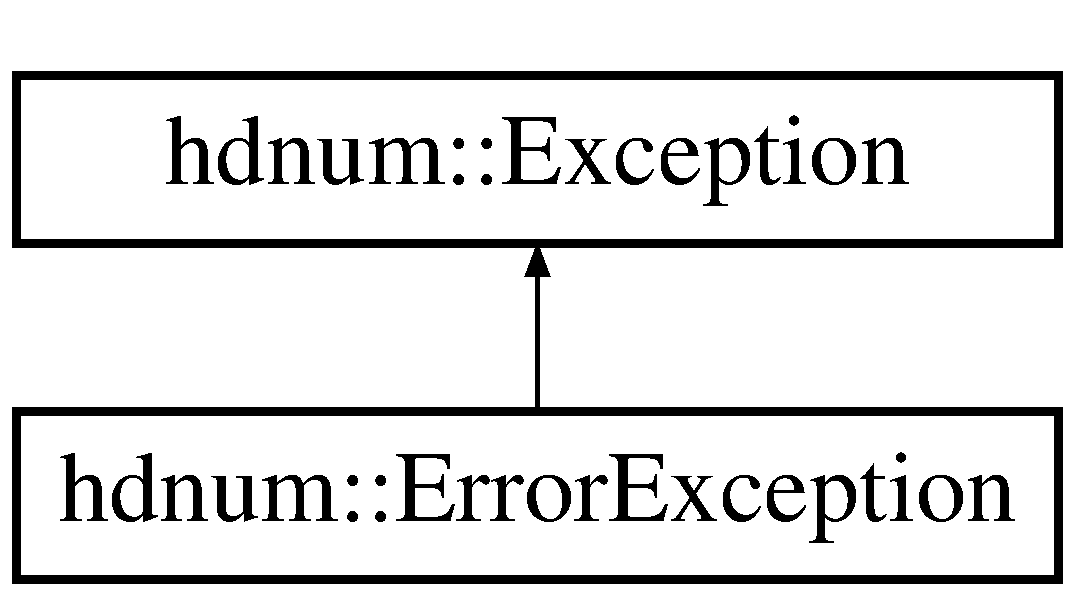
\includegraphics[height=2cm]{classhdnum_1_1ErrorException}
\end{center}
\end{figure}


\subsection{Detailed Description}
General Error. 

The documentation for this class was generated from the following file:\begin{DoxyCompactItemize}
\item 
src/\hyperlink{exceptions_8hh}{exceptions.hh}\end{DoxyCompactItemize}

\hypertarget{classhdnum_1_1Exception}{
\section{hdnum::Exception Class Reference}
\label{classhdnum_1_1Exception}\index{hdnum::Exception@{hdnum::Exception}}
}


Base class for Exceptions.  




{\ttfamily \#include $<$exceptions.hh$>$}

Inheritance diagram for hdnum::Exception:\begin{figure}[H]
\begin{center}
\leavevmode
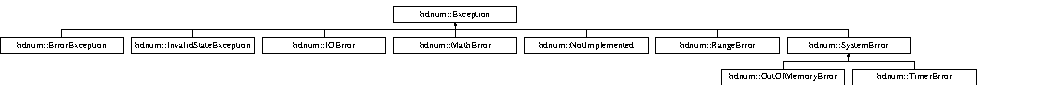
\includegraphics[height=1.14754cm]{classhdnum_1_1Exception}
\end{center}
\end{figure}
\subsection*{Public Member Functions}
\begin{DoxyCompactItemize}
\item 
\hypertarget{classhdnum_1_1Exception_a1761e43f1a7727c2ee39f32466df8c55}{
void \hyperlink{classhdnum_1_1Exception_a1761e43f1a7727c2ee39f32466df8c55}{message} (const std::string \&message)}
\label{classhdnum_1_1Exception_a1761e43f1a7727c2ee39f32466df8c55}

\begin{DoxyCompactList}\small\item\em store string in internal message buffer \item\end{DoxyCompactList}\item 
\hypertarget{classhdnum_1_1Exception_aa6f1c6150981b76282a20440c9b5e8ab}{
const std::string \& \hyperlink{classhdnum_1_1Exception_aa6f1c6150981b76282a20440c9b5e8ab}{what} () const }
\label{classhdnum_1_1Exception_aa6f1c6150981b76282a20440c9b5e8ab}

\begin{DoxyCompactList}\small\item\em output internal message buffer \item\end{DoxyCompactList}\end{DoxyCompactItemize}


\subsection{Detailed Description}
Base class for Exceptions. all HDNUM exceptions are derived from this class via trivial subclassing:


\begin{DoxyCode}
        class MyException : public Dune::Exception {};
\end{DoxyCode}


You should not {\ttfamily throw} a Dune::Exception directly but use the macro DUNE\_\-THROW() instead which fills the message-\/buffer of the exception in a standard way and features a way to pass the result in the operator$<$$<$-\/style

\begin{DoxySeeAlso}{See also}
\hyperlink{exceptions_8hh_a7385bc4ca18aaff3f509a30bde2567c0}{HDNUM\_\-THROW}, \hyperlink{classhdnum_1_1IOError}{IOError}, \hyperlink{classhdnum_1_1MathError}{MathError} 
\end{DoxySeeAlso}


The documentation for this class was generated from the following file:\begin{DoxyCompactItemize}
\item 
src/\hyperlink{exceptions_8hh}{exceptions.hh}\end{DoxyCompactItemize}

\hypertarget{classhdnum_1_1Heun2}{
\section{hdnum::Heun2$<$ M $>$ Class Template Reference}
\label{classhdnum_1_1Heun2}\index{hdnum::Heun2@{hdnum::Heun2}}
}


Heun method (order 2 with 2 stages).  




{\ttfamily \#include $<$ode.hh$>$}

\subsection*{Public Types}
\begin{DoxyCompactItemize}
\item 
\hypertarget{classhdnum_1_1Heun2_a32d59e62cf1c8dcc50cd2583fae3bf09}{
typedef M::size\_\-type \hyperlink{classhdnum_1_1Heun2_a32d59e62cf1c8dcc50cd2583fae3bf09}{size\_\-type}}
\label{classhdnum_1_1Heun2_a32d59e62cf1c8dcc50cd2583fae3bf09}

\begin{DoxyCompactList}\small\item\em export size\_\-type \item\end{DoxyCompactList}\item 
\hypertarget{classhdnum_1_1Heun2_ac2e59a8551ffbce1455c0fd5266965fd}{
typedef M::time\_\-type \hyperlink{classhdnum_1_1Heun2_ac2e59a8551ffbce1455c0fd5266965fd}{time\_\-type}}
\label{classhdnum_1_1Heun2_ac2e59a8551ffbce1455c0fd5266965fd}

\begin{DoxyCompactList}\small\item\em export time\_\-type \item\end{DoxyCompactList}\item 
\hypertarget{classhdnum_1_1Heun2_af16dadf05575fe6ec2c0602fedfe8d2b}{
typedef M::number\_\-type \hyperlink{classhdnum_1_1Heun2_af16dadf05575fe6ec2c0602fedfe8d2b}{number\_\-type}}
\label{classhdnum_1_1Heun2_af16dadf05575fe6ec2c0602fedfe8d2b}

\begin{DoxyCompactList}\small\item\em export number\_\-type \item\end{DoxyCompactList}\end{DoxyCompactItemize}
\subsection*{Public Member Functions}
\begin{DoxyCompactItemize}
\item 
\hypertarget{classhdnum_1_1Heun2_aeddfa6a0a287892a6008da5c95d13dd7}{
\hyperlink{classhdnum_1_1Heun2_aeddfa6a0a287892a6008da5c95d13dd7}{Heun2} (const M \&model\_\-)}
\label{classhdnum_1_1Heun2_aeddfa6a0a287892a6008da5c95d13dd7}

\begin{DoxyCompactList}\small\item\em constructor stores reference to the model \item\end{DoxyCompactList}\item 
\hypertarget{classhdnum_1_1Heun2_a4998cbb9dc1e4aa127a2209a5d5cb69c}{
void \hyperlink{classhdnum_1_1Heun2_a4998cbb9dc1e4aa127a2209a5d5cb69c}{set\_\-dt} (\hyperlink{classhdnum_1_1Heun2_ac2e59a8551ffbce1455c0fd5266965fd}{time\_\-type} dt\_\-)}
\label{classhdnum_1_1Heun2_a4998cbb9dc1e4aa127a2209a5d5cb69c}

\begin{DoxyCompactList}\small\item\em set time step for subsequent steps \item\end{DoxyCompactList}\item 
\hypertarget{classhdnum_1_1Heun2_a967c7c1e842f5400d568ebf0b7c92877}{
void \hyperlink{classhdnum_1_1Heun2_a967c7c1e842f5400d568ebf0b7c92877}{step} ()}
\label{classhdnum_1_1Heun2_a967c7c1e842f5400d568ebf0b7c92877}

\begin{DoxyCompactList}\small\item\em do one step \item\end{DoxyCompactList}\item 
\hypertarget{classhdnum_1_1Heun2_ad5f075aa349590dbfb2e99fc565dadfc}{
void \hyperlink{classhdnum_1_1Heun2_ad5f075aa349590dbfb2e99fc565dadfc}{set\_\-state} (\hyperlink{classhdnum_1_1Heun2_ac2e59a8551ffbce1455c0fd5266965fd}{time\_\-type} t\_\-, const \hyperlink{classhdnum_1_1Vector}{Vector}$<$ \hyperlink{classhdnum_1_1Heun2_af16dadf05575fe6ec2c0602fedfe8d2b}{number\_\-type} $>$ \&u\_\-)}
\label{classhdnum_1_1Heun2_ad5f075aa349590dbfb2e99fc565dadfc}

\begin{DoxyCompactList}\small\item\em set current state \item\end{DoxyCompactList}\item 
\hypertarget{classhdnum_1_1Heun2_ad14ab9cd78584ada47e543820bb73b78}{
const \hyperlink{classhdnum_1_1Vector}{Vector}$<$ \hyperlink{classhdnum_1_1Heun2_af16dadf05575fe6ec2c0602fedfe8d2b}{number\_\-type} $>$ \& \hyperlink{classhdnum_1_1Heun2_ad14ab9cd78584ada47e543820bb73b78}{get\_\-state} () const }
\label{classhdnum_1_1Heun2_ad14ab9cd78584ada47e543820bb73b78}

\begin{DoxyCompactList}\small\item\em get current state \item\end{DoxyCompactList}\item 
\hypertarget{classhdnum_1_1Heun2_a5ad86e97fa21759e935b1e79b7ff4029}{
\hyperlink{classhdnum_1_1Heun2_ac2e59a8551ffbce1455c0fd5266965fd}{time\_\-type} \hyperlink{classhdnum_1_1Heun2_a5ad86e97fa21759e935b1e79b7ff4029}{get\_\-time} () const }
\label{classhdnum_1_1Heun2_a5ad86e97fa21759e935b1e79b7ff4029}

\begin{DoxyCompactList}\small\item\em get current time \item\end{DoxyCompactList}\item 
\hypertarget{classhdnum_1_1Heun2_abde1a7c6195ecfd92184ed9d08173806}{
\hyperlink{classhdnum_1_1Heun2_ac2e59a8551ffbce1455c0fd5266965fd}{time\_\-type} \hyperlink{classhdnum_1_1Heun2_abde1a7c6195ecfd92184ed9d08173806}{get\_\-dt} () const }
\label{classhdnum_1_1Heun2_abde1a7c6195ecfd92184ed9d08173806}

\begin{DoxyCompactList}\small\item\em get dt used in last step (i.e. to compute current state) \item\end{DoxyCompactList}\item 
\hypertarget{classhdnum_1_1Heun2_a943af41b853f8b3d37e1889a6e60a17b}{
\hyperlink{classhdnum_1_1Heun2_a32d59e62cf1c8dcc50cd2583fae3bf09}{size\_\-type} \hyperlink{classhdnum_1_1Heun2_a943af41b853f8b3d37e1889a6e60a17b}{get\_\-order} () const }
\label{classhdnum_1_1Heun2_a943af41b853f8b3d37e1889a6e60a17b}

\begin{DoxyCompactList}\small\item\em return consistency order of the method \item\end{DoxyCompactList}\end{DoxyCompactItemize}


\subsection{Detailed Description}
\subsubsection*{template$<$class M$>$ class hdnum::Heun2$<$ M $>$}

Heun method (order 2 with 2 stages). The ODE solver is parametrized by a model. The model also exports all relevant types for time and states. The ODE solver encapsulates the states needed for the computation.


\begin{DoxyTemplParams}{Template Parameters}
\item[{\em M}]the model type \end{DoxyTemplParams}


The documentation for this class was generated from the following file:\begin{DoxyCompactItemize}
\item 
src/\hyperlink{ode_8hh}{ode.hh}\end{DoxyCompactItemize}

\hypertarget{classhdnum_1_1Heun3}{
\section{hdnum::Heun3$<$ M $>$ Class Template Reference}
\label{classhdnum_1_1Heun3}\index{hdnum::Heun3@{hdnum::Heun3}}
}


Heun method (order 3 with 3 stages).  




{\ttfamily \#include $<$ode.hh$>$}

\subsection*{Public Types}
\begin{DoxyCompactItemize}
\item 
\hypertarget{classhdnum_1_1Heun3_a99b9c3470be12f9c3e5e3804e77ec316}{
typedef M::size\_\-type \hyperlink{classhdnum_1_1Heun3_a99b9c3470be12f9c3e5e3804e77ec316}{size\_\-type}}
\label{classhdnum_1_1Heun3_a99b9c3470be12f9c3e5e3804e77ec316}

\begin{DoxyCompactList}\small\item\em export size\_\-type \item\end{DoxyCompactList}\item 
\hypertarget{classhdnum_1_1Heun3_a48fcfee8624c3e7984dc054d641ff962}{
typedef M::time\_\-type \hyperlink{classhdnum_1_1Heun3_a48fcfee8624c3e7984dc054d641ff962}{time\_\-type}}
\label{classhdnum_1_1Heun3_a48fcfee8624c3e7984dc054d641ff962}

\begin{DoxyCompactList}\small\item\em export time\_\-type \item\end{DoxyCompactList}\item 
\hypertarget{classhdnum_1_1Heun3_a4cda69fda9bfa3fb9d2a0ddeca50a29c}{
typedef M::number\_\-type \hyperlink{classhdnum_1_1Heun3_a4cda69fda9bfa3fb9d2a0ddeca50a29c}{number\_\-type}}
\label{classhdnum_1_1Heun3_a4cda69fda9bfa3fb9d2a0ddeca50a29c}

\begin{DoxyCompactList}\small\item\em export number\_\-type \item\end{DoxyCompactList}\end{DoxyCompactItemize}
\subsection*{Public Member Functions}
\begin{DoxyCompactItemize}
\item 
\hypertarget{classhdnum_1_1Heun3_a9994c2f6785c02199cbd2a35e9634a84}{
\hyperlink{classhdnum_1_1Heun3_a9994c2f6785c02199cbd2a35e9634a84}{Heun3} (const M \&model\_\-)}
\label{classhdnum_1_1Heun3_a9994c2f6785c02199cbd2a35e9634a84}

\begin{DoxyCompactList}\small\item\em constructor stores reference to the model \item\end{DoxyCompactList}\item 
\hypertarget{classhdnum_1_1Heun3_a438edc59b90c9a09b80f3d09c865bbda}{
void \hyperlink{classhdnum_1_1Heun3_a438edc59b90c9a09b80f3d09c865bbda}{set\_\-dt} (\hyperlink{classhdnum_1_1Heun3_a48fcfee8624c3e7984dc054d641ff962}{time\_\-type} dt\_\-)}
\label{classhdnum_1_1Heun3_a438edc59b90c9a09b80f3d09c865bbda}

\begin{DoxyCompactList}\small\item\em set time step for subsequent steps \item\end{DoxyCompactList}\item 
\hypertarget{classhdnum_1_1Heun3_ae216ddb0bf8459656dfb62c0a2fd1e69}{
void \hyperlink{classhdnum_1_1Heun3_ae216ddb0bf8459656dfb62c0a2fd1e69}{step} ()}
\label{classhdnum_1_1Heun3_ae216ddb0bf8459656dfb62c0a2fd1e69}

\begin{DoxyCompactList}\small\item\em do one step \item\end{DoxyCompactList}\item 
\hypertarget{classhdnum_1_1Heun3_a81644f725426f0aa5bb8ed5dc6d03cec}{
void \hyperlink{classhdnum_1_1Heun3_a81644f725426f0aa5bb8ed5dc6d03cec}{set\_\-state} (\hyperlink{classhdnum_1_1Heun3_a48fcfee8624c3e7984dc054d641ff962}{time\_\-type} t\_\-, const \hyperlink{classhdnum_1_1Vector}{Vector}$<$ \hyperlink{classhdnum_1_1Heun3_a4cda69fda9bfa3fb9d2a0ddeca50a29c}{number\_\-type} $>$ \&u\_\-)}
\label{classhdnum_1_1Heun3_a81644f725426f0aa5bb8ed5dc6d03cec}

\begin{DoxyCompactList}\small\item\em set current state \item\end{DoxyCompactList}\item 
\hypertarget{classhdnum_1_1Heun3_a776797bef464c76c1f7caa1f43bc9ccf}{
const \hyperlink{classhdnum_1_1Vector}{Vector}$<$ \hyperlink{classhdnum_1_1Heun3_a4cda69fda9bfa3fb9d2a0ddeca50a29c}{number\_\-type} $>$ \& \hyperlink{classhdnum_1_1Heun3_a776797bef464c76c1f7caa1f43bc9ccf}{get\_\-state} () const }
\label{classhdnum_1_1Heun3_a776797bef464c76c1f7caa1f43bc9ccf}

\begin{DoxyCompactList}\small\item\em get current state \item\end{DoxyCompactList}\item 
\hypertarget{classhdnum_1_1Heun3_ad5438e8365dba3b2cc885a4d22fe0789}{
\hyperlink{classhdnum_1_1Heun3_a48fcfee8624c3e7984dc054d641ff962}{time\_\-type} \hyperlink{classhdnum_1_1Heun3_ad5438e8365dba3b2cc885a4d22fe0789}{get\_\-time} () const }
\label{classhdnum_1_1Heun3_ad5438e8365dba3b2cc885a4d22fe0789}

\begin{DoxyCompactList}\small\item\em get current time \item\end{DoxyCompactList}\item 
\hypertarget{classhdnum_1_1Heun3_a55e46de6d92d67c40ee2aa84cbc4a8d7}{
\hyperlink{classhdnum_1_1Heun3_a48fcfee8624c3e7984dc054d641ff962}{time\_\-type} \hyperlink{classhdnum_1_1Heun3_a55e46de6d92d67c40ee2aa84cbc4a8d7}{get\_\-dt} () const }
\label{classhdnum_1_1Heun3_a55e46de6d92d67c40ee2aa84cbc4a8d7}

\begin{DoxyCompactList}\small\item\em get dt used in last step (i.e. to compute current state) \item\end{DoxyCompactList}\item 
\hypertarget{classhdnum_1_1Heun3_ab6db7ad9e5a6db68e23782dd83200d86}{
\hyperlink{classhdnum_1_1Heun3_a99b9c3470be12f9c3e5e3804e77ec316}{size\_\-type} \hyperlink{classhdnum_1_1Heun3_ab6db7ad9e5a6db68e23782dd83200d86}{get\_\-order} () const }
\label{classhdnum_1_1Heun3_ab6db7ad9e5a6db68e23782dd83200d86}

\begin{DoxyCompactList}\small\item\em return consistency order of the method \item\end{DoxyCompactList}\end{DoxyCompactItemize}


\subsection{Detailed Description}
\subsubsection*{template$<$class M$>$ class hdnum::Heun3$<$ M $>$}

Heun method (order 3 with 3 stages). The ODE solver is parametrized by a model. The model also exports all relevant types for time and states. The ODE solver encapsulates the states needed for the computation.


\begin{DoxyTemplParams}{Template Parameters}
\item[{\em M}]the model type \end{DoxyTemplParams}


The documentation for this class was generated from the following file:\begin{DoxyCompactItemize}
\item 
src/\hyperlink{ode_8hh}{ode.hh}\end{DoxyCompactItemize}

\hypertarget{classhdnum_1_1IE}{
\section{hdnum::IE$<$ M, S $>$ Class Template Reference}
\label{classhdnum_1_1IE}\index{hdnum::IE@{hdnum::IE}}
}


Implicit Euler using Newton's method to solve nonlinear system.  




{\ttfamily \#include $<$ode.hh$>$}

\subsection*{Classes}
\begin{DoxyCompactItemize}
\item 
class {\bfseries NonlinearProblem}
\begin{DoxyCompactList}\small\item\em class providing nonlinear problem to be solved \item\end{DoxyCompactList}\end{DoxyCompactItemize}
\subsection*{Public Types}
\begin{DoxyCompactItemize}
\item 
\hypertarget{classhdnum_1_1IE_af2d3dd8c57bb78dfd28a613dd11f499a}{
typedef M::size\_\-type \hyperlink{classhdnum_1_1IE_af2d3dd8c57bb78dfd28a613dd11f499a}{size\_\-type}}
\label{classhdnum_1_1IE_af2d3dd8c57bb78dfd28a613dd11f499a}

\begin{DoxyCompactList}\small\item\em export size\_\-type \item\end{DoxyCompactList}\item 
\hypertarget{classhdnum_1_1IE_a4a58f86ec61809cbca7b16922dcbb39e}{
typedef M::time\_\-type \hyperlink{classhdnum_1_1IE_a4a58f86ec61809cbca7b16922dcbb39e}{time\_\-type}}
\label{classhdnum_1_1IE_a4a58f86ec61809cbca7b16922dcbb39e}

\begin{DoxyCompactList}\small\item\em export time\_\-type \item\end{DoxyCompactList}\item 
\hypertarget{classhdnum_1_1IE_a23de7a983f5419c37d8530d49cab4913}{
typedef M::number\_\-type \hyperlink{classhdnum_1_1IE_a23de7a983f5419c37d8530d49cab4913}{number\_\-type}}
\label{classhdnum_1_1IE_a23de7a983f5419c37d8530d49cab4913}

\begin{DoxyCompactList}\small\item\em export number\_\-type \item\end{DoxyCompactList}\end{DoxyCompactItemize}
\subsection*{Public Member Functions}
\begin{DoxyCompactItemize}
\item 
\hypertarget{classhdnum_1_1IE_a25d8827c46865a4b6dae56a07b70f507}{
\hyperlink{classhdnum_1_1IE_a25d8827c46865a4b6dae56a07b70f507}{IE} (const M \&model\_\-, const S \&newton\_\-)}
\label{classhdnum_1_1IE_a25d8827c46865a4b6dae56a07b70f507}

\begin{DoxyCompactList}\small\item\em constructor stores reference to the model \item\end{DoxyCompactList}\item 
\hypertarget{classhdnum_1_1IE_a26bfa23447038750257ecdf75d341283}{
void \hyperlink{classhdnum_1_1IE_a26bfa23447038750257ecdf75d341283}{set\_\-dt} (\hyperlink{classhdnum_1_1IE_a4a58f86ec61809cbca7b16922dcbb39e}{time\_\-type} dt\_\-)}
\label{classhdnum_1_1IE_a26bfa23447038750257ecdf75d341283}

\begin{DoxyCompactList}\small\item\em set time step for subsequent steps \item\end{DoxyCompactList}\item 
\hypertarget{classhdnum_1_1IE_a3ece1463453f15fe247c030e487ea232}{
void \hyperlink{classhdnum_1_1IE_a3ece1463453f15fe247c030e487ea232}{set\_\-verbosity} (\hyperlink{classhdnum_1_1IE_af2d3dd8c57bb78dfd28a613dd11f499a}{size\_\-type} verbosity\_\-)}
\label{classhdnum_1_1IE_a3ece1463453f15fe247c030e487ea232}

\begin{DoxyCompactList}\small\item\em set verbosity level \item\end{DoxyCompactList}\item 
\hypertarget{classhdnum_1_1IE_a947a239a2ddfe6d3f946db28f04a900d}{
void \hyperlink{classhdnum_1_1IE_a947a239a2ddfe6d3f946db28f04a900d}{step} ()}
\label{classhdnum_1_1IE_a947a239a2ddfe6d3f946db28f04a900d}

\begin{DoxyCompactList}\small\item\em do one step \item\end{DoxyCompactList}\item 
\hypertarget{classhdnum_1_1IE_a69b53dd12e5b00739b26551102c090bb}{
bool \hyperlink{classhdnum_1_1IE_a69b53dd12e5b00739b26551102c090bb}{get\_\-error} () const }
\label{classhdnum_1_1IE_a69b53dd12e5b00739b26551102c090bb}

\begin{DoxyCompactList}\small\item\em get current state \item\end{DoxyCompactList}\item 
\hypertarget{classhdnum_1_1IE_aa333a60e09305968c3ae333a06c5abd4}{
void \hyperlink{classhdnum_1_1IE_aa333a60e09305968c3ae333a06c5abd4}{set\_\-state} (\hyperlink{classhdnum_1_1IE_a4a58f86ec61809cbca7b16922dcbb39e}{time\_\-type} t\_\-, const \hyperlink{classhdnum_1_1Vector}{Vector}$<$ \hyperlink{classhdnum_1_1IE_a23de7a983f5419c37d8530d49cab4913}{number\_\-type} $>$ \&u\_\-)}
\label{classhdnum_1_1IE_aa333a60e09305968c3ae333a06c5abd4}

\begin{DoxyCompactList}\small\item\em set current state \item\end{DoxyCompactList}\item 
\hypertarget{classhdnum_1_1IE_a7c9b9284e27f01f67f776f7e6b5c4cf7}{
const \hyperlink{classhdnum_1_1Vector}{Vector}$<$ \hyperlink{classhdnum_1_1IE_a23de7a983f5419c37d8530d49cab4913}{number\_\-type} $>$ \& \hyperlink{classhdnum_1_1IE_a7c9b9284e27f01f67f776f7e6b5c4cf7}{get\_\-state} () const }
\label{classhdnum_1_1IE_a7c9b9284e27f01f67f776f7e6b5c4cf7}

\begin{DoxyCompactList}\small\item\em get current state \item\end{DoxyCompactList}\item 
\hypertarget{classhdnum_1_1IE_a2abb282e43dc676c2b192f49e732986a}{
\hyperlink{classhdnum_1_1IE_a4a58f86ec61809cbca7b16922dcbb39e}{time\_\-type} \hyperlink{classhdnum_1_1IE_a2abb282e43dc676c2b192f49e732986a}{get\_\-time} () const }
\label{classhdnum_1_1IE_a2abb282e43dc676c2b192f49e732986a}

\begin{DoxyCompactList}\small\item\em get current time \item\end{DoxyCompactList}\item 
\hypertarget{classhdnum_1_1IE_aeaea0a1cdee7135d0e85e980c4f15179}{
\hyperlink{classhdnum_1_1IE_a4a58f86ec61809cbca7b16922dcbb39e}{time\_\-type} \hyperlink{classhdnum_1_1IE_aeaea0a1cdee7135d0e85e980c4f15179}{get\_\-dt} () const }
\label{classhdnum_1_1IE_aeaea0a1cdee7135d0e85e980c4f15179}

\begin{DoxyCompactList}\small\item\em get dt used in last step (i.e. to compute current state) \item\end{DoxyCompactList}\item 
\hypertarget{classhdnum_1_1IE_acbc50aab0984aa2fc0d59ad02fb530fb}{
\hyperlink{classhdnum_1_1IE_af2d3dd8c57bb78dfd28a613dd11f499a}{size\_\-type} \hyperlink{classhdnum_1_1IE_acbc50aab0984aa2fc0d59ad02fb530fb}{get\_\-order} () const }
\label{classhdnum_1_1IE_acbc50aab0984aa2fc0d59ad02fb530fb}

\begin{DoxyCompactList}\small\item\em return consistency order of the method \item\end{DoxyCompactList}\item 
\hypertarget{classhdnum_1_1IE_ac0cc9141ec0c29ea465ffc4b416a52a8}{
void \hyperlink{classhdnum_1_1IE_ac0cc9141ec0c29ea465ffc4b416a52a8}{get\_\-info} () const }
\label{classhdnum_1_1IE_ac0cc9141ec0c29ea465ffc4b416a52a8}

\begin{DoxyCompactList}\small\item\em print some information \item\end{DoxyCompactList}\end{DoxyCompactItemize}


\subsection{Detailed Description}
\subsubsection*{template$<$class M, class S$>$ class hdnum::IE$<$ M, S $>$}

Implicit Euler using Newton's method to solve nonlinear system. The ODE solver is parametrized by a model. The model also exports all relevant types for time and states. The ODE solver encapsulates the states needed for the computation.


\begin{DoxyTemplParams}{Template Parameters}
\item[{\em M}]the model type \item[{\em S}]nonlinear solver \end{DoxyTemplParams}


The documentation for this class was generated from the following file:\begin{DoxyCompactItemize}
\item 
src/\hyperlink{ode_8hh}{ode.hh}\end{DoxyCompactItemize}

\hypertarget{classhdnum_1_1InvalidStateException}{
\section{hdnum::InvalidStateException Class Reference}
\label{classhdnum_1_1InvalidStateException}\index{hdnum::InvalidStateException@{hdnum::InvalidStateException}}
}


Default exception if a function was called while the object is not in a valid state for that function.  




{\ttfamily \#include $<$exceptions.hh$>$}

Inheritance diagram for hdnum::InvalidStateException:\begin{figure}[H]
\begin{center}
\leavevmode
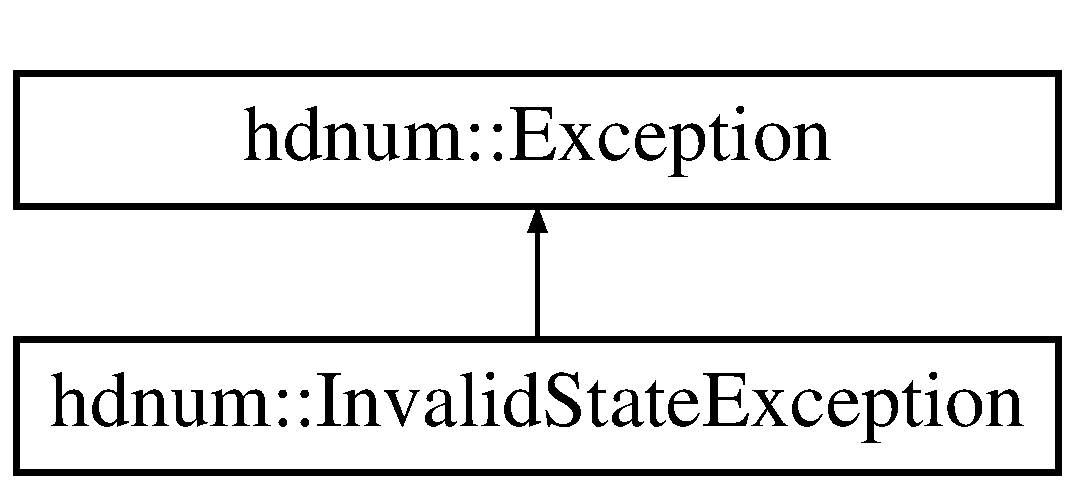
\includegraphics[height=2cm]{classhdnum_1_1InvalidStateException}
\end{center}
\end{figure}


\subsection{Detailed Description}
Default exception if a function was called while the object is not in a valid state for that function. 

The documentation for this class was generated from the following file:\begin{DoxyCompactItemize}
\item 
src/\hyperlink{exceptions_8hh}{exceptions.hh}\end{DoxyCompactItemize}

\hypertarget{classhdnum_1_1IOError}{
\section{hdnum::IOError Class Reference}
\label{classhdnum_1_1IOError}\index{hdnum::IOError@{hdnum::IOError}}
}


Default exception class for I/O errors.  




{\ttfamily \#include $<$exceptions.hh$>$}

Inheritance diagram for hdnum::IOError:\begin{figure}[H]
\begin{center}
\leavevmode
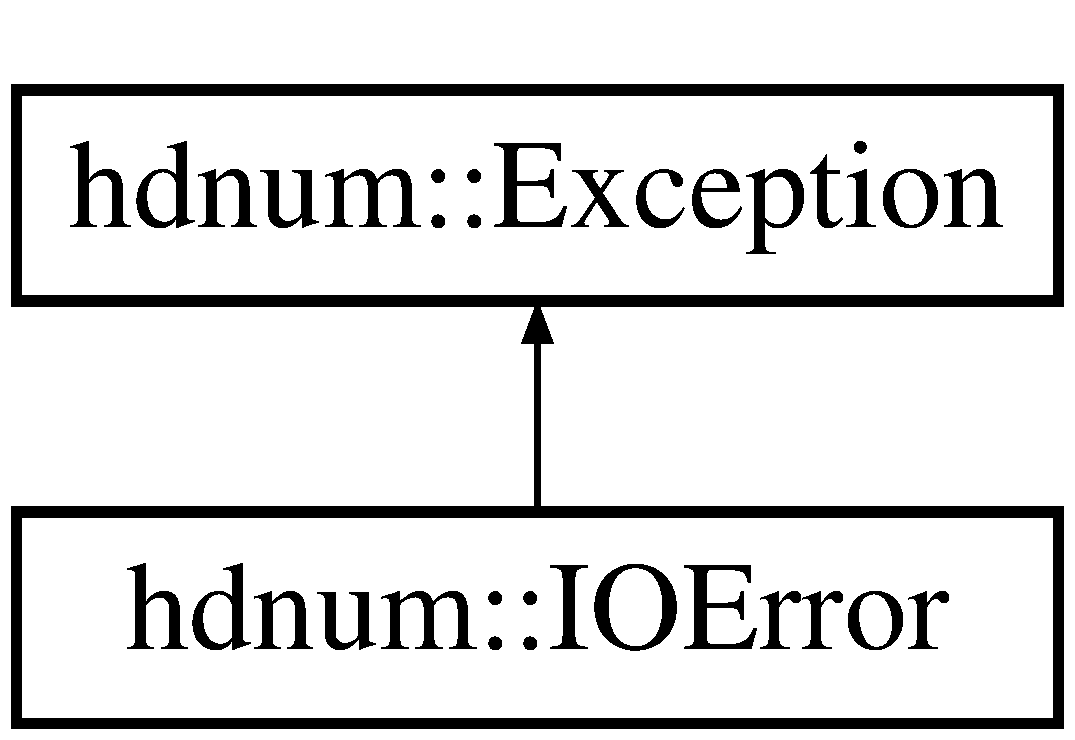
\includegraphics[height=2cm]{classhdnum_1_1IOError}
\end{center}
\end{figure}


\subsection{Detailed Description}
Default exception class for I/O errors. This is a superclass for any errors dealing with file/socket I/O problems like


\begin{DoxyItemize}
\item file not found
\item could not write file
\item could not connect to remote socket 
\end{DoxyItemize}

The documentation for this class was generated from the following file:\begin{DoxyCompactItemize}
\item 
src/\hyperlink{exceptions_8hh}{exceptions.hh}\end{DoxyCompactItemize}

\hypertarget{classhdnum_1_1Kutta3}{
\section{hdnum::Kutta3$<$ M $>$ Class Template Reference}
\label{classhdnum_1_1Kutta3}\index{hdnum::Kutta3@{hdnum::Kutta3}}
}


Kutta method (order 3 with 3 stages).  




{\ttfamily \#include $<$ode.hh$>$}

\subsection*{Public Types}
\begin{DoxyCompactItemize}
\item 
\hypertarget{classhdnum_1_1Kutta3_aa219675a459b3d48c8ac301a1f6d712b}{
typedef M::size\_\-type \hyperlink{classhdnum_1_1Kutta3_aa219675a459b3d48c8ac301a1f6d712b}{size\_\-type}}
\label{classhdnum_1_1Kutta3_aa219675a459b3d48c8ac301a1f6d712b}

\begin{DoxyCompactList}\small\item\em export size\_\-type \item\end{DoxyCompactList}\item 
\hypertarget{classhdnum_1_1Kutta3_a0055d10b545c5cf60a16fd3a88a6042e}{
typedef M::time\_\-type \hyperlink{classhdnum_1_1Kutta3_a0055d10b545c5cf60a16fd3a88a6042e}{time\_\-type}}
\label{classhdnum_1_1Kutta3_a0055d10b545c5cf60a16fd3a88a6042e}

\begin{DoxyCompactList}\small\item\em export time\_\-type \item\end{DoxyCompactList}\item 
\hypertarget{classhdnum_1_1Kutta3_a06dc1fee934f3a4cbb530f4bc4704b99}{
typedef M::number\_\-type \hyperlink{classhdnum_1_1Kutta3_a06dc1fee934f3a4cbb530f4bc4704b99}{number\_\-type}}
\label{classhdnum_1_1Kutta3_a06dc1fee934f3a4cbb530f4bc4704b99}

\begin{DoxyCompactList}\small\item\em export number\_\-type \item\end{DoxyCompactList}\end{DoxyCompactItemize}
\subsection*{Public Member Functions}
\begin{DoxyCompactItemize}
\item 
\hypertarget{classhdnum_1_1Kutta3_af743deba93833d61ae035a5c3eb5b563}{
\hyperlink{classhdnum_1_1Kutta3_af743deba93833d61ae035a5c3eb5b563}{Kutta3} (const M \&model\_\-)}
\label{classhdnum_1_1Kutta3_af743deba93833d61ae035a5c3eb5b563}

\begin{DoxyCompactList}\small\item\em constructor stores reference to the model \item\end{DoxyCompactList}\item 
\hypertarget{classhdnum_1_1Kutta3_ac5b0e2c4ae00e3d3faf7d83351f76866}{
void \hyperlink{classhdnum_1_1Kutta3_ac5b0e2c4ae00e3d3faf7d83351f76866}{set\_\-dt} (\hyperlink{classhdnum_1_1Kutta3_a0055d10b545c5cf60a16fd3a88a6042e}{time\_\-type} dt\_\-)}
\label{classhdnum_1_1Kutta3_ac5b0e2c4ae00e3d3faf7d83351f76866}

\begin{DoxyCompactList}\small\item\em set time step for subsequent steps \item\end{DoxyCompactList}\item 
\hypertarget{classhdnum_1_1Kutta3_a5c97bd9408b64f29052781b8a62180b4}{
void \hyperlink{classhdnum_1_1Kutta3_a5c97bd9408b64f29052781b8a62180b4}{step} ()}
\label{classhdnum_1_1Kutta3_a5c97bd9408b64f29052781b8a62180b4}

\begin{DoxyCompactList}\small\item\em do one step \item\end{DoxyCompactList}\item 
\hypertarget{classhdnum_1_1Kutta3_a474ab02413887a0c1fadb81a7e4fb851}{
void \hyperlink{classhdnum_1_1Kutta3_a474ab02413887a0c1fadb81a7e4fb851}{set\_\-state} (\hyperlink{classhdnum_1_1Kutta3_a0055d10b545c5cf60a16fd3a88a6042e}{time\_\-type} t\_\-, const \hyperlink{classhdnum_1_1Vector}{Vector}$<$ \hyperlink{classhdnum_1_1Kutta3_a06dc1fee934f3a4cbb530f4bc4704b99}{number\_\-type} $>$ \&u\_\-)}
\label{classhdnum_1_1Kutta3_a474ab02413887a0c1fadb81a7e4fb851}

\begin{DoxyCompactList}\small\item\em set current state \item\end{DoxyCompactList}\item 
\hypertarget{classhdnum_1_1Kutta3_add2141212e9549fd50e15deedf892b3e}{
const \hyperlink{classhdnum_1_1Vector}{Vector}$<$ \hyperlink{classhdnum_1_1Kutta3_a06dc1fee934f3a4cbb530f4bc4704b99}{number\_\-type} $>$ \& \hyperlink{classhdnum_1_1Kutta3_add2141212e9549fd50e15deedf892b3e}{get\_\-state} () const }
\label{classhdnum_1_1Kutta3_add2141212e9549fd50e15deedf892b3e}

\begin{DoxyCompactList}\small\item\em get current state \item\end{DoxyCompactList}\item 
\hypertarget{classhdnum_1_1Kutta3_a11598389a3a0bd0403b2906c147640e2}{
\hyperlink{classhdnum_1_1Kutta3_a0055d10b545c5cf60a16fd3a88a6042e}{time\_\-type} \hyperlink{classhdnum_1_1Kutta3_a11598389a3a0bd0403b2906c147640e2}{get\_\-time} () const }
\label{classhdnum_1_1Kutta3_a11598389a3a0bd0403b2906c147640e2}

\begin{DoxyCompactList}\small\item\em get current time \item\end{DoxyCompactList}\item 
\hypertarget{classhdnum_1_1Kutta3_a365f2f78d21f7db184a88665ac1f9b58}{
\hyperlink{classhdnum_1_1Kutta3_a0055d10b545c5cf60a16fd3a88a6042e}{time\_\-type} \hyperlink{classhdnum_1_1Kutta3_a365f2f78d21f7db184a88665ac1f9b58}{get\_\-dt} () const }
\label{classhdnum_1_1Kutta3_a365f2f78d21f7db184a88665ac1f9b58}

\begin{DoxyCompactList}\small\item\em get dt used in last step (i.e. to compute current state) \item\end{DoxyCompactList}\item 
\hypertarget{classhdnum_1_1Kutta3_a47f10303531b80d34d84cbae496b0543}{
\hyperlink{classhdnum_1_1Kutta3_aa219675a459b3d48c8ac301a1f6d712b}{size\_\-type} \hyperlink{classhdnum_1_1Kutta3_a47f10303531b80d34d84cbae496b0543}{get\_\-order} () const }
\label{classhdnum_1_1Kutta3_a47f10303531b80d34d84cbae496b0543}

\begin{DoxyCompactList}\small\item\em return consistency order of the method \item\end{DoxyCompactList}\end{DoxyCompactItemize}


\subsection{Detailed Description}
\subsubsection*{template$<$class M$>$ class hdnum::Kutta3$<$ M $>$}

Kutta method (order 3 with 3 stages). The ODE solver is parametrized by a model. The model also exports all relevant types for time and states. The ODE solver encapsulates the states needed for the computation.


\begin{DoxyTemplParams}{Template Parameters}
\item[{\em M}]the model type \end{DoxyTemplParams}


The documentation for this class was generated from the following file:\begin{DoxyCompactItemize}
\item 
src/\hyperlink{ode_8hh}{ode.hh}\end{DoxyCompactItemize}

\hypertarget{classhdnum_1_1MathError}{
\section{hdnum::MathError Class Reference}
\label{classhdnum_1_1MathError}\index{hdnum::MathError@{hdnum::MathError}}
}


Default exception class for mathematical errors.  




{\ttfamily \#include $<$exceptions.hh$>$}

Inheritance diagram for hdnum::MathError:\begin{figure}[H]
\begin{center}
\leavevmode
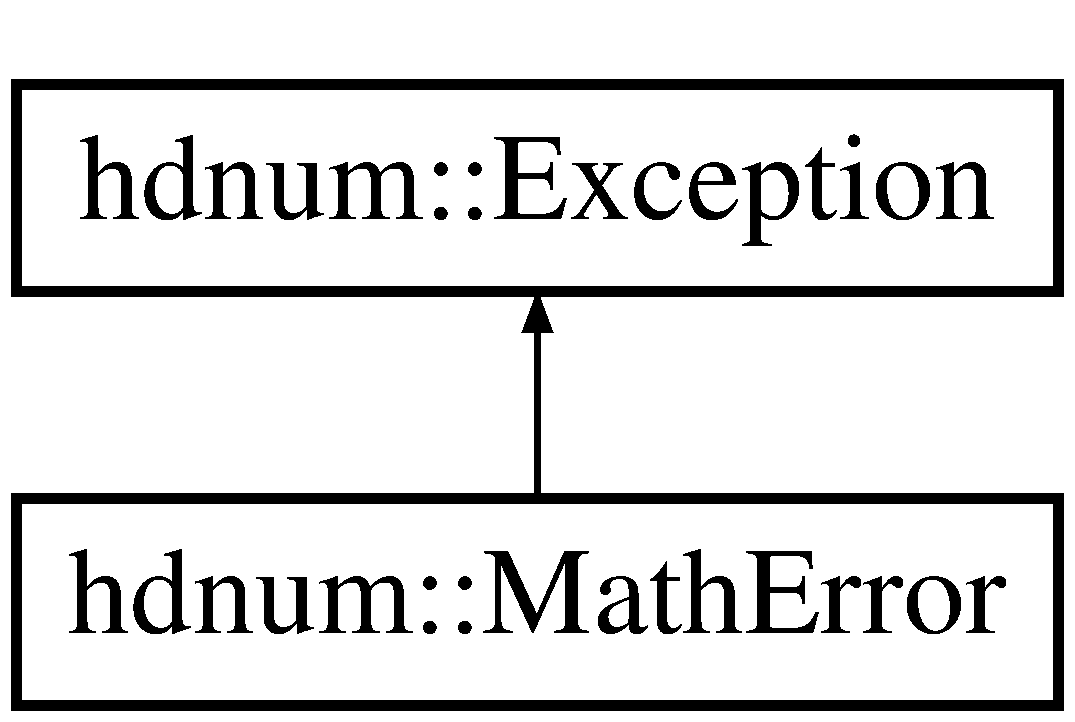
\includegraphics[height=2cm]{classhdnum_1_1MathError}
\end{center}
\end{figure}


\subsection{Detailed Description}
Default exception class for mathematical errors. This is the superclass for all errors which are caused by mathematical problems like


\begin{DoxyItemize}
\item matrix not invertible
\item not convergent 
\end{DoxyItemize}

The documentation for this class was generated from the following file:\begin{DoxyCompactItemize}
\item 
src/\hyperlink{exceptions_8hh}{exceptions.hh}\end{DoxyCompactItemize}

\hypertarget{classhdnum_1_1Matrix}{
\section{hdnum::Matrix$<$ T $>$ Class Template Reference}
\label{classhdnum_1_1Matrix}\index{hdnum::Matrix@{hdnum::Matrix}}
}


A flexible matrix class.  




{\ttfamily \#include $<$matrix.hh$>$}

\subsection*{Public Types}
\begin{DoxyCompactItemize}
\item 
\hypertarget{classhdnum_1_1Matrix_a6ebaff96f20f8e78a454ffabdd7723f6}{
typedef T \hyperlink{classhdnum_1_1Matrix_a6ebaff96f20f8e78a454ffabdd7723f6}{value\_\-type}}
\label{classhdnum_1_1Matrix_a6ebaff96f20f8e78a454ffabdd7723f6}

\begin{DoxyCompactList}\small\item\em Remember the storage type. \item\end{DoxyCompactList}\item 
\hypertarget{classhdnum_1_1Matrix_ad41eb9538a08f24849a7b68b4732e0bf}{
typedef \hyperlink{classhdnum_1_1Matrix_a6ebaff96f20f8e78a454ffabdd7723f6}{value\_\-type} \& \hyperlink{classhdnum_1_1Matrix_ad41eb9538a08f24849a7b68b4732e0bf}{reference}}
\label{classhdnum_1_1Matrix_ad41eb9538a08f24849a7b68b4732e0bf}

\begin{DoxyCompactList}\small\item\em Reference to an object. \item\end{DoxyCompactList}\item 
\hypertarget{classhdnum_1_1Matrix_a20309dda0b0e95081958c7d3235e2c20}{
typedef const \hyperlink{classhdnum_1_1Matrix_a6ebaff96f20f8e78a454ffabdd7723f6}{value\_\-type} \& \hyperlink{classhdnum_1_1Matrix_a20309dda0b0e95081958c7d3235e2c20}{const\_\-reference}}
\label{classhdnum_1_1Matrix_a20309dda0b0e95081958c7d3235e2c20}

\begin{DoxyCompactList}\small\item\em Const reference to an object. \item\end{DoxyCompactList}\item 
\hypertarget{classhdnum_1_1Matrix_adeafaf5fa5732e0d67f90ffa2119fbf1}{
typedef std::size\_\-t \hyperlink{classhdnum_1_1Matrix_adeafaf5fa5732e0d67f90ffa2119fbf1}{size\_\-type}}
\label{classhdnum_1_1Matrix_adeafaf5fa5732e0d67f90ffa2119fbf1}

\begin{DoxyCompactList}\small\item\em Type used for array indices. \item\end{DoxyCompactList}\item 
\hypertarget{classhdnum_1_1Matrix_a32f25247f12a8913e8db646c539f1dbd}{
typedef std::ptrdiff\_\-t \hyperlink{classhdnum_1_1Matrix_a32f25247f12a8913e8db646c539f1dbd}{difference\_\-type}}
\label{classhdnum_1_1Matrix_a32f25247f12a8913e8db646c539f1dbd}

\begin{DoxyCompactList}\small\item\em Difference type. \item\end{DoxyCompactList}\end{DoxyCompactItemize}
\subsection*{Public Member Functions}
\begin{DoxyCompactItemize}
\item 
\hypertarget{classhdnum_1_1Matrix_ae8abe838fca01e6f98811c68b807fdb7}{
\hyperlink{classhdnum_1_1Matrix_ae8abe838fca01e6f98811c68b807fdb7}{Matrix} ()}
\label{classhdnum_1_1Matrix_ae8abe838fca01e6f98811c68b807fdb7}

\begin{DoxyCompactList}\small\item\em make empty matrix \item\end{DoxyCompactList}\item 
\hypertarget{classhdnum_1_1Matrix_afe276ea428efa8a82dc2eaa2bf35ff57}{
\hyperlink{classhdnum_1_1Matrix_afe276ea428efa8a82dc2eaa2bf35ff57}{Matrix} (\hyperlink{classhdnum_1_1Matrix_adeafaf5fa5732e0d67f90ffa2119fbf1}{size\_\-type} \_\-m, \hyperlink{classhdnum_1_1Matrix_adeafaf5fa5732e0d67f90ffa2119fbf1}{size\_\-type} \_\-n)}
\label{classhdnum_1_1Matrix_afe276ea428efa8a82dc2eaa2bf35ff57}

\begin{DoxyCompactList}\small\item\em make \_\-m x \_\-n matrix uninitialized \item\end{DoxyCompactList}\item 
\hypertarget{classhdnum_1_1Matrix_a59a74b9437fba7526e8dcec22adafa74}{
\hyperlink{classhdnum_1_1Matrix_a59a74b9437fba7526e8dcec22adafa74}{Matrix} (\hyperlink{classhdnum_1_1Matrix_adeafaf5fa5732e0d67f90ffa2119fbf1}{size\_\-type} \_\-m, \hyperlink{classhdnum_1_1Matrix_adeafaf5fa5732e0d67f90ffa2119fbf1}{size\_\-type} \_\-n, const T \&\_\-t)}
\label{classhdnum_1_1Matrix_a59a74b9437fba7526e8dcec22adafa74}

\begin{DoxyCompactList}\small\item\em make \_\-m x \_\-n matrix initialized \item\end{DoxyCompactList}\item 
\hypertarget{classhdnum_1_1Matrix_aa274920768bfee886c06f52638b068f7}{
\hyperlink{classhdnum_1_1Matrix_aa274920768bfee886c06f52638b068f7}{Matrix} (const \hyperlink{classhdnum_1_1Matrix}{Matrix} \&A)}
\label{classhdnum_1_1Matrix_aa274920768bfee886c06f52638b068f7}

\begin{DoxyCompactList}\small\item\em copy constructor with reference semantics \item\end{DoxyCompactList}\item 
\hypertarget{classhdnum_1_1Matrix_ad069ec9fdbef159b0069e325bd9bc064}{
\hyperlink{classhdnum_1_1Matrix}{Matrix} \& \hyperlink{classhdnum_1_1Matrix_ad069ec9fdbef159b0069e325bd9bc064}{operator=} (const \hyperlink{classhdnum_1_1Matrix}{Matrix} \&A)}
\label{classhdnum_1_1Matrix_ad069ec9fdbef159b0069e325bd9bc064}

\begin{DoxyCompactList}\small\item\em assignment operator assumes that argument has exactly the same size \item\end{DoxyCompactList}\item 
\hypertarget{classhdnum_1_1Matrix_a5ee9bbcecaa5fca03210f40e4d9f9b35}{
\hyperlink{classhdnum_1_1Matrix}{Matrix} \& \hyperlink{classhdnum_1_1Matrix_a5ee9bbcecaa5fca03210f40e4d9f9b35}{operator=} (const T \&t)}
\label{classhdnum_1_1Matrix_a5ee9bbcecaa5fca03210f40e4d9f9b35}

\begin{DoxyCompactList}\small\item\em assignment from scalar \item\end{DoxyCompactList}\item 
\hypertarget{classhdnum_1_1Matrix_a25e70187797f88c4ccf2f68fe79a7e86}{
\hyperlink{classhdnum_1_1Matrix}{Matrix}$<$ T $>$ \hyperlink{classhdnum_1_1Matrix_a25e70187797f88c4ccf2f68fe79a7e86}{sub} (\hyperlink{classhdnum_1_1Matrix_adeafaf5fa5732e0d67f90ffa2119fbf1}{size\_\-type} i, \hyperlink{classhdnum_1_1Matrix_adeafaf5fa5732e0d67f90ffa2119fbf1}{size\_\-type} j, \hyperlink{classhdnum_1_1Matrix_adeafaf5fa5732e0d67f90ffa2119fbf1}{size\_\-type} rows, \hyperlink{classhdnum_1_1Matrix_adeafaf5fa5732e0d67f90ffa2119fbf1}{size\_\-type} cols)}
\label{classhdnum_1_1Matrix_a25e70187797f88c4ccf2f68fe79a7e86}

\begin{DoxyCompactList}\small\item\em submatrix extraction \item\end{DoxyCompactList}\item 
\hypertarget{classhdnum_1_1Matrix_a70d073fcf197cf4ac085bb667b156ba3}{
T $\ast$ \hyperlink{classhdnum_1_1Matrix_a70d073fcf197cf4ac085bb667b156ba3}{operator\mbox{[}$\,$\mbox{]}} (\hyperlink{classhdnum_1_1Matrix_adeafaf5fa5732e0d67f90ffa2119fbf1}{size\_\-type} i)}
\label{classhdnum_1_1Matrix_a70d073fcf197cf4ac085bb667b156ba3}

\begin{DoxyCompactList}\small\item\em Component access. \item\end{DoxyCompactList}\item 
\hypertarget{classhdnum_1_1Matrix_acd7aa64f80d71dabe9f7d02749dd067e}{
const T $\ast$ \hyperlink{classhdnum_1_1Matrix_acd7aa64f80d71dabe9f7d02749dd067e}{operator\mbox{[}$\,$\mbox{]}} (\hyperlink{classhdnum_1_1Matrix_adeafaf5fa5732e0d67f90ffa2119fbf1}{size\_\-type} i) const }
\label{classhdnum_1_1Matrix_acd7aa64f80d71dabe9f7d02749dd067e}

\begin{DoxyCompactList}\small\item\em Component access. \item\end{DoxyCompactList}\item 
\hyperlink{classhdnum_1_1Matrix}{Matrix} \& \hyperlink{classhdnum_1_1Matrix_a4f3f23f9a07540723601283d034c10ae}{operator+=} (const \hyperlink{classhdnum_1_1Matrix}{Matrix} \&B)
\begin{DoxyCompactList}\small\item\em Addition assignment. \item\end{DoxyCompactList}\item 
\hyperlink{classhdnum_1_1Matrix}{Matrix} \& \hyperlink{classhdnum_1_1Matrix_acbc74183e387ce2bc40fa3d785e75a83}{operator-\/=} (const \hyperlink{classhdnum_1_1Matrix}{Matrix} \&B)
\begin{DoxyCompactList}\small\item\em Subtraction assignment. \item\end{DoxyCompactList}\item 
\hyperlink{classhdnum_1_1Matrix}{Matrix} \& \hyperlink{classhdnum_1_1Matrix_adc378774314424fd9c5600bc34bed356}{operator$\ast$=} (const T \&s)
\begin{DoxyCompactList}\small\item\em Scalar multiplication assignment. \item\end{DoxyCompactList}\item 
\hyperlink{classhdnum_1_1Matrix}{Matrix} \& \hyperlink{classhdnum_1_1Matrix_ac4850f9b5df8da4a8fb40ddf05a3ed39}{operator/=} (const T \&s)
\begin{DoxyCompactList}\small\item\em Scalar division assignment. \item\end{DoxyCompactList}\item 
void \hyperlink{classhdnum_1_1Matrix_acb2eaf3fb83498d4c7b2de964c5e53de}{update} (const T \&s, const \hyperlink{classhdnum_1_1Matrix}{Matrix} \&B)
\begin{DoxyCompactList}\small\item\em Scaled update of a \hyperlink{classhdnum_1_1Matrix}{Matrix}. \item\end{DoxyCompactList}\item 
\hypertarget{classhdnum_1_1Matrix_abd684181d36b38464d2b58827f95fec3}{
{\footnotesize template$<$class V $>$ }\\void \hyperlink{classhdnum_1_1Matrix_abd684181d36b38464d2b58827f95fec3}{mv} (\hyperlink{classhdnum_1_1Vector}{Vector}$<$ V $>$ \&y, const \hyperlink{classhdnum_1_1Vector}{Vector}$<$ V $>$ \&x) const }
\label{classhdnum_1_1Matrix_abd684181d36b38464d2b58827f95fec3}

\begin{DoxyCompactList}\small\item\em matrix vector product y = A$\ast$x \item\end{DoxyCompactList}\item 
\hypertarget{classhdnum_1_1Matrix_a907264ce1afd644a9b6ef10756b3dcd3}{
{\footnotesize template$<$class V $>$ }\\void \hyperlink{classhdnum_1_1Matrix_a907264ce1afd644a9b6ef10756b3dcd3}{umv} (\hyperlink{classhdnum_1_1Vector}{Vector}$<$ V $>$ \&y, const \hyperlink{classhdnum_1_1Vector}{Vector}$<$ V $>$ \&x) const }
\label{classhdnum_1_1Matrix_a907264ce1afd644a9b6ef10756b3dcd3}

\begin{DoxyCompactList}\small\item\em update matrix vector product y += A$\ast$x \item\end{DoxyCompactList}\item 
\hypertarget{classhdnum_1_1Matrix_a7eee0aa57c0ea42edc1419031887364a}{
{\footnotesize template$<$class V $>$ }\\void \hyperlink{classhdnum_1_1Matrix_a7eee0aa57c0ea42edc1419031887364a}{umv} (\hyperlink{classhdnum_1_1Vector}{Vector}$<$ V $>$ \&y, const V \&s, const \hyperlink{classhdnum_1_1Vector}{Vector}$<$ V $>$ \&x) const }
\label{classhdnum_1_1Matrix_a7eee0aa57c0ea42edc1419031887364a}

\begin{DoxyCompactList}\small\item\em update matrix vector product y += A$\ast$x \item\end{DoxyCompactList}\item 
\hypertarget{classhdnum_1_1Matrix_a42d98f6f42d831ee37c602951503a808}{
void \hyperlink{classhdnum_1_1Matrix_a42d98f6f42d831ee37c602951503a808}{mm} (const \hyperlink{classhdnum_1_1Matrix}{Matrix}$<$ T $>$ \&A, const \hyperlink{classhdnum_1_1Matrix}{Matrix}$<$ T $>$ \&B)}
\label{classhdnum_1_1Matrix_a42d98f6f42d831ee37c602951503a808}

\begin{DoxyCompactList}\small\item\em matrix matrix product C = A$\ast$B \item\end{DoxyCompactList}\item 
\hypertarget{classhdnum_1_1Matrix_a9c4539920d988a072fcb9582a64aaeef}{
void \hyperlink{classhdnum_1_1Matrix_a9c4539920d988a072fcb9582a64aaeef}{umm} (const \hyperlink{classhdnum_1_1Matrix}{Matrix}$<$ T $>$ \&A, const \hyperlink{classhdnum_1_1Matrix}{Matrix}$<$ T $>$ \&B)}
\label{classhdnum_1_1Matrix_a9c4539920d988a072fcb9582a64aaeef}

\begin{DoxyCompactList}\small\item\em matrix matrix product C += A$\ast$B \item\end{DoxyCompactList}\item 
\hypertarget{classhdnum_1_1Matrix_aaa1dfa0cd2e96e07799e1ae1d1a3d8d0}{
void \hyperlink{classhdnum_1_1Matrix_aaa1dfa0cd2e96e07799e1ae1d1a3d8d0}{sc} (const \hyperlink{classhdnum_1_1Vector}{Vector}$<$ T $>$ \&x, \hyperlink{classhdnum_1_1Matrix_adeafaf5fa5732e0d67f90ffa2119fbf1}{size\_\-type} k)}
\label{classhdnum_1_1Matrix_aaa1dfa0cd2e96e07799e1ae1d1a3d8d0}

\begin{DoxyCompactList}\small\item\em set column: make x the k'th column of A \item\end{DoxyCompactList}\item 
\hypertarget{classhdnum_1_1Matrix_ab274466f69f341a6a2dc18362284efe1}{
void \hyperlink{classhdnum_1_1Matrix_ab274466f69f341a6a2dc18362284efe1}{sr} (const \hyperlink{classhdnum_1_1Vector}{Vector}$<$ T $>$ \&x, \hyperlink{classhdnum_1_1Matrix_adeafaf5fa5732e0d67f90ffa2119fbf1}{size\_\-type} k)}
\label{classhdnum_1_1Matrix_ab274466f69f341a6a2dc18362284efe1}

\begin{DoxyCompactList}\small\item\em set row: make x the k'th row of A \item\end{DoxyCompactList}\item 
\hypertarget{classhdnum_1_1Matrix_a0ba1392f7d18208ca7940e2cff23599d}{
T \hyperlink{classhdnum_1_1Matrix_a0ba1392f7d18208ca7940e2cff23599d}{norm\_\-infty} () const }
\label{classhdnum_1_1Matrix_a0ba1392f7d18208ca7940e2cff23599d}

\begin{DoxyCompactList}\small\item\em compute row sum norm \item\end{DoxyCompactList}\item 
\hypertarget{classhdnum_1_1Matrix_a750b9da89753d0f90c349e5c406ba50a}{
T \hyperlink{classhdnum_1_1Matrix_a750b9da89753d0f90c349e5c406ba50a}{norm\_\-1} () const }
\label{classhdnum_1_1Matrix_a750b9da89753d0f90c349e5c406ba50a}

\begin{DoxyCompactList}\small\item\em compute column sum norm \item\end{DoxyCompactList}\item 
\hypertarget{classhdnum_1_1Matrix_a7fbe5bceef2d6577f8d68ca3c1216280}{
\hyperlink{classhdnum_1_1Matrix_adeafaf5fa5732e0d67f90ffa2119fbf1}{size\_\-type} \hyperlink{classhdnum_1_1Matrix_a7fbe5bceef2d6577f8d68ca3c1216280}{rowsize} () const }
\label{classhdnum_1_1Matrix_a7fbe5bceef2d6577f8d68ca3c1216280}

\begin{DoxyCompactList}\small\item\em get number of rows \item\end{DoxyCompactList}\item 
\hypertarget{classhdnum_1_1Matrix_af0a22e4c87c7097af07f5bc6307f470b}{
\hyperlink{classhdnum_1_1Matrix_adeafaf5fa5732e0d67f90ffa2119fbf1}{size\_\-type} \hyperlink{classhdnum_1_1Matrix_af0a22e4c87c7097af07f5bc6307f470b}{colsize} () const }
\label{classhdnum_1_1Matrix_af0a22e4c87c7097af07f5bc6307f470b}

\begin{DoxyCompactList}\small\item\em get number of columns \item\end{DoxyCompactList}\item 
\hypertarget{classhdnum_1_1Matrix_a743699a7471dc4ac86edb3e01cbf251d}{
int \hyperlink{classhdnum_1_1Matrix_a743699a7471dc4ac86edb3e01cbf251d}{iwidth} () const }
\label{classhdnum_1_1Matrix_a743699a7471dc4ac86edb3e01cbf251d}

\begin{DoxyCompactList}\small\item\em get index field width for pretty-\/printing \item\end{DoxyCompactList}\item 
\hypertarget{classhdnum_1_1Matrix_ad2280e529019e6bda5940904068ca82d}{
int \hyperlink{classhdnum_1_1Matrix_ad2280e529019e6bda5940904068ca82d}{width} () const }
\label{classhdnum_1_1Matrix_ad2280e529019e6bda5940904068ca82d}

\begin{DoxyCompactList}\small\item\em get data field width for pretty-\/printing \item\end{DoxyCompactList}\item 
\hypertarget{classhdnum_1_1Matrix_a1fdd89980844347b3b5d752bc97be2c3}{
int \hyperlink{classhdnum_1_1Matrix_a1fdd89980844347b3b5d752bc97be2c3}{precision} () const }
\label{classhdnum_1_1Matrix_a1fdd89980844347b3b5d752bc97be2c3}

\begin{DoxyCompactList}\small\item\em get data precision for pretty-\/printing \item\end{DoxyCompactList}\item 
\hypertarget{classhdnum_1_1Matrix_a67f77c92267311fd152fc2b5d1dce406}{
void \hyperlink{classhdnum_1_1Matrix_a67f77c92267311fd152fc2b5d1dce406}{iwidth} (int i) const }
\label{classhdnum_1_1Matrix_a67f77c92267311fd152fc2b5d1dce406}

\begin{DoxyCompactList}\small\item\em set index field width for pretty-\/printing \item\end{DoxyCompactList}\item 
\hypertarget{classhdnum_1_1Matrix_a9985540222b45151bf160a4c1f0eb4ad}{
void \hyperlink{classhdnum_1_1Matrix_a9985540222b45151bf160a4c1f0eb4ad}{width} (int i) const }
\label{classhdnum_1_1Matrix_a9985540222b45151bf160a4c1f0eb4ad}

\begin{DoxyCompactList}\small\item\em set data field width for pretty-\/printing \item\end{DoxyCompactList}\item 
\hypertarget{classhdnum_1_1Matrix_aa4575ff95760bb69d7fb916bcfb3e18a}{
void \hyperlink{classhdnum_1_1Matrix_aa4575ff95760bb69d7fb916bcfb3e18a}{precision} (int i) const }
\label{classhdnum_1_1Matrix_aa4575ff95760bb69d7fb916bcfb3e18a}

\begin{DoxyCompactList}\small\item\em set data precision for pretty-\/printing \item\end{DoxyCompactList}\end{DoxyCompactItemize}


\subsection{Detailed Description}
\subsubsection*{template$<$class T$>$ class hdnum::Matrix$<$ T $>$}

A flexible matrix class. \hyperlink{classhdnum_1_1Matrix}{Matrix} is implemented as a handle to a dynamically allocated array. Copy and assignement operators have reference semantics. In order to make a true copy the function \char`\"{}copy\char`\"{} can be used. 

\subsection{Member Function Documentation}
\hypertarget{classhdnum_1_1Matrix_adc378774314424fd9c5600bc34bed356}{
\index{hdnum::Matrix@{hdnum::Matrix}!operator$\ast$=@{operator$\ast$=}}
\index{operator$\ast$=@{operator$\ast$=}!hdnum::Matrix@{hdnum::Matrix}}
\subsubsection[{operator$\ast$=}]{\setlength{\rightskip}{0pt plus 5cm}template$<$class T$>$ {\bf Matrix}\& {\bf hdnum::Matrix}$<$ T $>$::operator$\ast$= (const T \& {\em s})\hspace{0.3cm}{\ttfamily  \mbox{[}inline\mbox{]}}}}
\label{classhdnum_1_1Matrix_adc378774314424fd9c5600bc34bed356}


Scalar multiplication assignment. 

Implements A $\ast$= s where s is a scalar


\begin{DoxyParams}{Parameters}
\item[\mbox{$\leftarrow$} {\em s}]scalar value to multiply with vector scalar multiplication \end{DoxyParams}
\hypertarget{classhdnum_1_1Matrix_a4f3f23f9a07540723601283d034c10ae}{
\index{hdnum::Matrix@{hdnum::Matrix}!operator+=@{operator+=}}
\index{operator+=@{operator+=}!hdnum::Matrix@{hdnum::Matrix}}
\subsubsection[{operator+=}]{\setlength{\rightskip}{0pt plus 5cm}template$<$class T$>$ {\bf Matrix}\& {\bf hdnum::Matrix}$<$ T $>$::operator+= (const {\bf Matrix}$<$ T $>$ \& {\em B})\hspace{0.3cm}{\ttfamily  \mbox{[}inline\mbox{]}}}}
\label{classhdnum_1_1Matrix_a4f3f23f9a07540723601283d034c10ae}


Addition assignment. 

Implements A += B matrix addition


\begin{DoxyParams}{Parameters}
\item[\mbox{$\leftarrow$} {\em B}]another \hyperlink{classhdnum_1_1Matrix}{Matrix} \end{DoxyParams}
\hypertarget{classhdnum_1_1Matrix_acbc74183e387ce2bc40fa3d785e75a83}{
\index{hdnum::Matrix@{hdnum::Matrix}!operator-\/=@{operator-\/=}}
\index{operator-\/=@{operator-\/=}!hdnum::Matrix@{hdnum::Matrix}}
\subsubsection[{operator-\/=}]{\setlength{\rightskip}{0pt plus 5cm}template$<$class T$>$ {\bf Matrix}\& {\bf hdnum::Matrix}$<$ T $>$::operator-\/= (const {\bf Matrix}$<$ T $>$ \& {\em B})\hspace{0.3cm}{\ttfamily  \mbox{[}inline\mbox{]}}}}
\label{classhdnum_1_1Matrix_acbc74183e387ce2bc40fa3d785e75a83}


Subtraction assignment. 

Implements A -\/= B matrix subtraction


\begin{DoxyParams}{Parameters}
\item[\mbox{$\leftarrow$} {\em B}]another matrix \end{DoxyParams}
\hypertarget{classhdnum_1_1Matrix_ac4850f9b5df8da4a8fb40ddf05a3ed39}{
\index{hdnum::Matrix@{hdnum::Matrix}!operator/=@{operator/=}}
\index{operator/=@{operator/=}!hdnum::Matrix@{hdnum::Matrix}}
\subsubsection[{operator/=}]{\setlength{\rightskip}{0pt plus 5cm}template$<$class T$>$ {\bf Matrix}\& {\bf hdnum::Matrix}$<$ T $>$::operator/= (const T \& {\em s})\hspace{0.3cm}{\ttfamily  \mbox{[}inline\mbox{]}}}}
\label{classhdnum_1_1Matrix_ac4850f9b5df8da4a8fb40ddf05a3ed39}


Scalar division assignment. 

Implements A /= s where s is a scalar


\begin{DoxyParams}{Parameters}
\item[\mbox{$\leftarrow$} {\em s}]scalar value to multiply with vector scalar multiplication \end{DoxyParams}
\hypertarget{classhdnum_1_1Matrix_acb2eaf3fb83498d4c7b2de964c5e53de}{
\index{hdnum::Matrix@{hdnum::Matrix}!update@{update}}
\index{update@{update}!hdnum::Matrix@{hdnum::Matrix}}
\subsubsection[{update}]{\setlength{\rightskip}{0pt plus 5cm}template$<$class T$>$ void {\bf hdnum::Matrix}$<$ T $>$::update (const T \& {\em s}, \/  const {\bf Matrix}$<$ T $>$ \& {\em B})\hspace{0.3cm}{\ttfamily  \mbox{[}inline\mbox{]}}}}
\label{classhdnum_1_1Matrix_acb2eaf3fb83498d4c7b2de964c5e53de}


Scaled update of a \hyperlink{classhdnum_1_1Matrix}{Matrix}. 

Implements A += s$\ast$B where s is a scalar and B a matrix


\begin{DoxyParams}{Parameters}
\item[\mbox{$\leftarrow$} {\em s}]scalar value to multiply with \item[\mbox{$\leftarrow$} {\em B}]another matrix \end{DoxyParams}


The documentation for this class was generated from the following file:\begin{DoxyCompactItemize}
\item 
src/\hyperlink{matrix_8hh}{matrix.hh}\end{DoxyCompactItemize}

\hypertarget{classhdnum_1_1ModifiedEuler}{
\section{hdnum::ModifiedEuler$<$ M $>$ Class Template Reference}
\label{classhdnum_1_1ModifiedEuler}\index{hdnum::ModifiedEuler@{hdnum::ModifiedEuler}}
}


Modified Euler method (order 2 with 2 stages).  




{\ttfamily \#include $<$ode.hh$>$}

\subsection*{Public Types}
\begin{DoxyCompactItemize}
\item 
\hypertarget{classhdnum_1_1ModifiedEuler_aa8841e11397920c273afab1f9a04c9bd}{
typedef M::size\_\-type \hyperlink{classhdnum_1_1ModifiedEuler_aa8841e11397920c273afab1f9a04c9bd}{size\_\-type}}
\label{classhdnum_1_1ModifiedEuler_aa8841e11397920c273afab1f9a04c9bd}

\begin{DoxyCompactList}\small\item\em export size\_\-type \item\end{DoxyCompactList}\item 
\hypertarget{classhdnum_1_1ModifiedEuler_a1c273cddcddf36f6e47f713080c06b41}{
typedef M::time\_\-type \hyperlink{classhdnum_1_1ModifiedEuler_a1c273cddcddf36f6e47f713080c06b41}{time\_\-type}}
\label{classhdnum_1_1ModifiedEuler_a1c273cddcddf36f6e47f713080c06b41}

\begin{DoxyCompactList}\small\item\em export time\_\-type \item\end{DoxyCompactList}\item 
\hypertarget{classhdnum_1_1ModifiedEuler_abcfd3cb8a5b446f721582af3b170476e}{
typedef M::number\_\-type \hyperlink{classhdnum_1_1ModifiedEuler_abcfd3cb8a5b446f721582af3b170476e}{number\_\-type}}
\label{classhdnum_1_1ModifiedEuler_abcfd3cb8a5b446f721582af3b170476e}

\begin{DoxyCompactList}\small\item\em export number\_\-type \item\end{DoxyCompactList}\end{DoxyCompactItemize}
\subsection*{Public Member Functions}
\begin{DoxyCompactItemize}
\item 
\hypertarget{classhdnum_1_1ModifiedEuler_ac7ad8c2a695fa27a8666dd4cd5a2e105}{
\hyperlink{classhdnum_1_1ModifiedEuler_ac7ad8c2a695fa27a8666dd4cd5a2e105}{ModifiedEuler} (const M \&model\_\-)}
\label{classhdnum_1_1ModifiedEuler_ac7ad8c2a695fa27a8666dd4cd5a2e105}

\begin{DoxyCompactList}\small\item\em constructor stores reference to the model \item\end{DoxyCompactList}\item 
\hypertarget{classhdnum_1_1ModifiedEuler_ad40c382bf56183ddb0a86e327d3ac7ac}{
void \hyperlink{classhdnum_1_1ModifiedEuler_ad40c382bf56183ddb0a86e327d3ac7ac}{set\_\-dt} (\hyperlink{classhdnum_1_1ModifiedEuler_a1c273cddcddf36f6e47f713080c06b41}{time\_\-type} dt\_\-)}
\label{classhdnum_1_1ModifiedEuler_ad40c382bf56183ddb0a86e327d3ac7ac}

\begin{DoxyCompactList}\small\item\em set time step for subsequent steps \item\end{DoxyCompactList}\item 
\hypertarget{classhdnum_1_1ModifiedEuler_a1842b79faa9c19fb406c0dfe92ae613d}{
void \hyperlink{classhdnum_1_1ModifiedEuler_a1842b79faa9c19fb406c0dfe92ae613d}{step} ()}
\label{classhdnum_1_1ModifiedEuler_a1842b79faa9c19fb406c0dfe92ae613d}

\begin{DoxyCompactList}\small\item\em do one step \item\end{DoxyCompactList}\item 
\hypertarget{classhdnum_1_1ModifiedEuler_a5fed8e518bd7f3f12e58c1cc6e6121fb}{
void \hyperlink{classhdnum_1_1ModifiedEuler_a5fed8e518bd7f3f12e58c1cc6e6121fb}{set\_\-state} (\hyperlink{classhdnum_1_1ModifiedEuler_a1c273cddcddf36f6e47f713080c06b41}{time\_\-type} t\_\-, const \hyperlink{classhdnum_1_1Vector}{Vector}$<$ \hyperlink{classhdnum_1_1ModifiedEuler_abcfd3cb8a5b446f721582af3b170476e}{number\_\-type} $>$ \&u\_\-)}
\label{classhdnum_1_1ModifiedEuler_a5fed8e518bd7f3f12e58c1cc6e6121fb}

\begin{DoxyCompactList}\small\item\em set current state \item\end{DoxyCompactList}\item 
\hypertarget{classhdnum_1_1ModifiedEuler_ab73d18011b660a3e7b7c53caecac96b7}{
const \hyperlink{classhdnum_1_1Vector}{Vector}$<$ \hyperlink{classhdnum_1_1ModifiedEuler_abcfd3cb8a5b446f721582af3b170476e}{number\_\-type} $>$ \& \hyperlink{classhdnum_1_1ModifiedEuler_ab73d18011b660a3e7b7c53caecac96b7}{get\_\-state} () const }
\label{classhdnum_1_1ModifiedEuler_ab73d18011b660a3e7b7c53caecac96b7}

\begin{DoxyCompactList}\small\item\em get current state \item\end{DoxyCompactList}\item 
\hypertarget{classhdnum_1_1ModifiedEuler_a837697657a3543e87c4b3e15ceda8491}{
\hyperlink{classhdnum_1_1ModifiedEuler_a1c273cddcddf36f6e47f713080c06b41}{time\_\-type} \hyperlink{classhdnum_1_1ModifiedEuler_a837697657a3543e87c4b3e15ceda8491}{get\_\-time} () const }
\label{classhdnum_1_1ModifiedEuler_a837697657a3543e87c4b3e15ceda8491}

\begin{DoxyCompactList}\small\item\em get current time \item\end{DoxyCompactList}\item 
\hypertarget{classhdnum_1_1ModifiedEuler_a697a2e3423e5ba2a9bd41b61e1358da5}{
\hyperlink{classhdnum_1_1ModifiedEuler_a1c273cddcddf36f6e47f713080c06b41}{time\_\-type} \hyperlink{classhdnum_1_1ModifiedEuler_a697a2e3423e5ba2a9bd41b61e1358da5}{get\_\-dt} () const }
\label{classhdnum_1_1ModifiedEuler_a697a2e3423e5ba2a9bd41b61e1358da5}

\begin{DoxyCompactList}\small\item\em get dt used in last step (i.e. to compute current state) \item\end{DoxyCompactList}\item 
\hypertarget{classhdnum_1_1ModifiedEuler_abaf92ae2a3a462996b5208d326cc9a6b}{
\hyperlink{classhdnum_1_1ModifiedEuler_aa8841e11397920c273afab1f9a04c9bd}{size\_\-type} \hyperlink{classhdnum_1_1ModifiedEuler_abaf92ae2a3a462996b5208d326cc9a6b}{get\_\-order} () const }
\label{classhdnum_1_1ModifiedEuler_abaf92ae2a3a462996b5208d326cc9a6b}

\begin{DoxyCompactList}\small\item\em return consistency order of the method \item\end{DoxyCompactList}\end{DoxyCompactItemize}


\subsection{Detailed Description}
\subsubsection*{template$<$class M$>$ class hdnum::ModifiedEuler$<$ M $>$}

Modified Euler method (order 2 with 2 stages). The ODE solver is parametrized by a model. The model also exports all relevant types for time and states. The ODE solver encapsulates the states needed for the computation.


\begin{DoxyTemplParams}{Template Parameters}
\item[{\em M}]the model type \end{DoxyTemplParams}


The documentation for this class was generated from the following file:\begin{DoxyCompactItemize}
\item 
src/\hyperlink{ode_8hh}{ode.hh}\end{DoxyCompactItemize}

\hypertarget{classhdnum_1_1Newton}{
\section{hdnum::Newton Class Reference}
\label{classhdnum_1_1Newton}\index{hdnum::Newton@{hdnum::Newton}}
}


Solve nonlinear problem using a damped \hyperlink{classhdnum_1_1Newton}{Newton} method.  




{\ttfamily \#include $<$newton.hh$>$}

\subsection*{Public Member Functions}
\begin{DoxyCompactItemize}
\item 
\hypertarget{classhdnum_1_1Newton_aee062778e7fed23339a63ca5695e5a45}{
\hyperlink{classhdnum_1_1Newton_aee062778e7fed23339a63ca5695e5a45}{Newton} ()}
\label{classhdnum_1_1Newton_aee062778e7fed23339a63ca5695e5a45}

\begin{DoxyCompactList}\small\item\em constructor stores reference to the model \item\end{DoxyCompactList}\item 
\hypertarget{classhdnum_1_1Newton_a98bf335f10122b8199cd84c2d00b463e}{
void \hyperlink{classhdnum_1_1Newton_a98bf335f10122b8199cd84c2d00b463e}{set\_\-maxit} (size\_\-type n)}
\label{classhdnum_1_1Newton_a98bf335f10122b8199cd84c2d00b463e}

\begin{DoxyCompactList}\small\item\em maximum number of iterations before giving up \item\end{DoxyCompactList}\item 
\hypertarget{classhdnum_1_1Newton_a5f68ee3f5e2143b0c4f645ee9e42cdc3}{
void \hyperlink{classhdnum_1_1Newton_a5f68ee3f5e2143b0c4f645ee9e42cdc3}{set\_\-linesearchsteps} (size\_\-type n)}
\label{classhdnum_1_1Newton_a5f68ee3f5e2143b0c4f645ee9e42cdc3}

\begin{DoxyCompactList}\small\item\em maximum number of steps in linesearch before giving up \item\end{DoxyCompactList}\item 
\hypertarget{classhdnum_1_1Newton_a5d2e9decea2d4e71dc2d0a266c2e0010}{
void \hyperlink{classhdnum_1_1Newton_a5d2e9decea2d4e71dc2d0a266c2e0010}{set\_\-verbosity} (size\_\-type n)}
\label{classhdnum_1_1Newton_a5d2e9decea2d4e71dc2d0a266c2e0010}

\begin{DoxyCompactList}\small\item\em control output given 0=nothing, 1=summary, 2=every step, 3=include line search \item\end{DoxyCompactList}\item 
\hypertarget{classhdnum_1_1Newton_a4da35666f8794067a3ca84f1fea895f0}{
void \hyperlink{classhdnum_1_1Newton_a4da35666f8794067a3ca84f1fea895f0}{set\_\-abslimit} (double l)}
\label{classhdnum_1_1Newton_a4da35666f8794067a3ca84f1fea895f0}

\begin{DoxyCompactList}\small\item\em basolute limit for defect \item\end{DoxyCompactList}\item 
\hypertarget{classhdnum_1_1Newton_ac28cbdace309a823ddc62b6ed929dadc}{
void \hyperlink{classhdnum_1_1Newton_ac28cbdace309a823ddc62b6ed929dadc}{set\_\-reduction} (double l)}
\label{classhdnum_1_1Newton_ac28cbdace309a823ddc62b6ed929dadc}

\begin{DoxyCompactList}\small\item\em reduction factor \item\end{DoxyCompactList}\item 
\hypertarget{classhdnum_1_1Newton_ab4f4df87fbf938cf186530408bfab2b3}{
{\footnotesize template$<$class M $>$ }\\void \hyperlink{classhdnum_1_1Newton_ab4f4df87fbf938cf186530408bfab2b3}{solve} (const M \&model, \hyperlink{classhdnum_1_1Vector}{Vector}$<$ typename M::number\_\-type $>$ \&x) const }
\label{classhdnum_1_1Newton_ab4f4df87fbf938cf186530408bfab2b3}

\begin{DoxyCompactList}\small\item\em do one step \item\end{DoxyCompactList}\item 
\hypertarget{classhdnum_1_1Newton_a2f133f417aa9b71ad92d72d6935401fa}{
bool {\bfseries has\_\-converged} () const }
\label{classhdnum_1_1Newton_a2f133f417aa9b71ad92d72d6935401fa}

\end{DoxyCompactItemize}


\subsection{Detailed Description}
Solve nonlinear problem using a damped \hyperlink{classhdnum_1_1Newton}{Newton} method. The \hyperlink{classhdnum_1_1Newton}{Newton} solver is parametrized by a model. The model also exports all relevant types for types. 

The documentation for this class was generated from the following file:\begin{DoxyCompactItemize}
\item 
src/\hyperlink{newton_8hh}{newton.hh}\end{DoxyCompactItemize}

\hypertarget{classhdnum_1_1NondeletingMemoryManagementPolicy}{
\section{hdnum::NondeletingMemoryManagementPolicy Class Reference}
\label{classhdnum_1_1NondeletingMemoryManagementPolicy}\index{hdnum::NondeletingMemoryManagementPolicy@{hdnum::NondeletingMemoryManagementPolicy}}
}


Don't delete target if reference count reaches zero.  




{\ttfamily \#include $<$countingptr.hh$>$}

\subsection*{Static Public Member Functions}
\begin{DoxyCompactItemize}
\item 
\hypertarget{classhdnum_1_1NondeletingMemoryManagementPolicy_a52e5e801b0796943f7d06a341d8c1ab4}{
{\footnotesize template$<$typename T $>$ }\\static void {\bfseries delete\_\-action} (T $\ast$p)}
\label{classhdnum_1_1NondeletingMemoryManagementPolicy_a52e5e801b0796943f7d06a341d8c1ab4}

\end{DoxyCompactItemize}


\subsection{Detailed Description}
Don't delete target if reference count reaches zero. If this class is given to \hyperlink{classhdnum_1_1CP}{CP} as the memory management policy, the \hyperlink{classhdnum_1_1CP}{CP} objects won't delete the pointed to object if the reference count reaches zero. 

The documentation for this class was generated from the following file:\begin{DoxyCompactItemize}
\item 
src/\hyperlink{countingptr_8hh}{countingptr.hh}\end{DoxyCompactItemize}

\hypertarget{classhdnum_1_1NotImplemented}{
\section{hdnum::NotImplemented Class Reference}
\label{classhdnum_1_1NotImplemented}\index{hdnum::NotImplemented@{hdnum::NotImplemented}}
}


Default exception for dummy implementations.  




{\ttfamily \#include $<$exceptions.hh$>$}

Inheritance diagram for hdnum::NotImplemented:\begin{figure}[H]
\begin{center}
\leavevmode
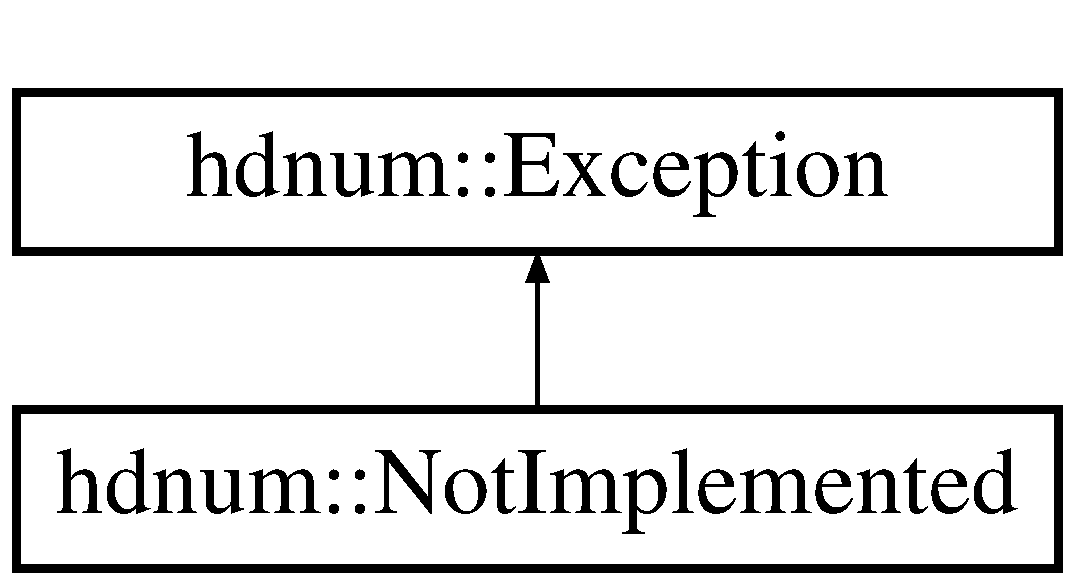
\includegraphics[height=2cm]{classhdnum_1_1NotImplemented}
\end{center}
\end{figure}


\subsection{Detailed Description}
Default exception for dummy implementations. This exception can be used for functions/methods


\begin{DoxyItemize}
\item that have to be implemented but should never be called
\item that are missing 
\end{DoxyItemize}

The documentation for this class was generated from the following file:\begin{DoxyCompactItemize}
\item 
src/\hyperlink{exceptions_8hh}{exceptions.hh}\end{DoxyCompactItemize}

\hypertarget{classhdnum_1_1OutOfMemoryError}{
\section{hdnum::OutOfMemoryError Class Reference}
\label{classhdnum_1_1OutOfMemoryError}\index{hdnum::OutOfMemoryError@{hdnum::OutOfMemoryError}}
}


Default exception if memory allocation fails.  




{\ttfamily \#include $<$exceptions.hh$>$}

Inheritance diagram for hdnum::OutOfMemoryError:\begin{figure}[H]
\begin{center}
\leavevmode
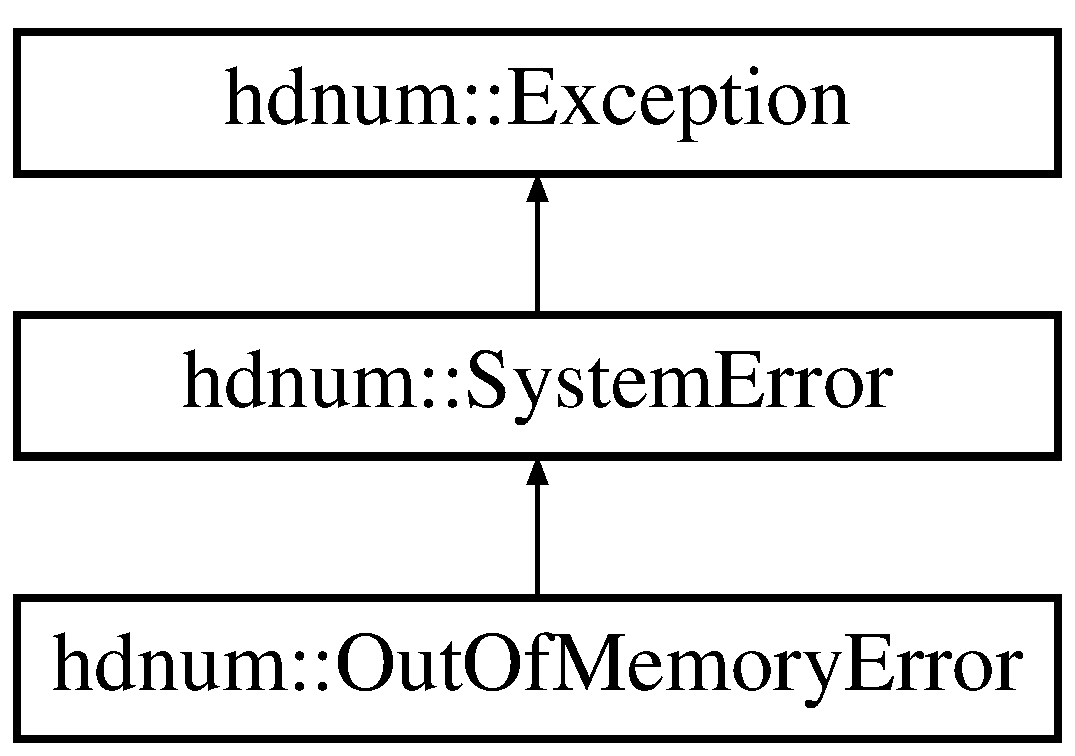
\includegraphics[height=3cm]{classhdnum_1_1OutOfMemoryError}
\end{center}
\end{figure}


\subsection{Detailed Description}
Default exception if memory allocation fails. 

The documentation for this class was generated from the following file:\begin{DoxyCompactItemize}
\item 
src/\hyperlink{exceptions_8hh}{exceptions.hh}\end{DoxyCompactItemize}

\hypertarget{classhdnum_1_1RangeError}{
\section{hdnum::RangeError Class Reference}
\label{classhdnum_1_1RangeError}\index{hdnum::RangeError@{hdnum::RangeError}}
}


Default exception class for range errors.  




{\ttfamily \#include $<$exceptions.hh$>$}

Inheritance diagram for hdnum::RangeError:\begin{figure}[H]
\begin{center}
\leavevmode
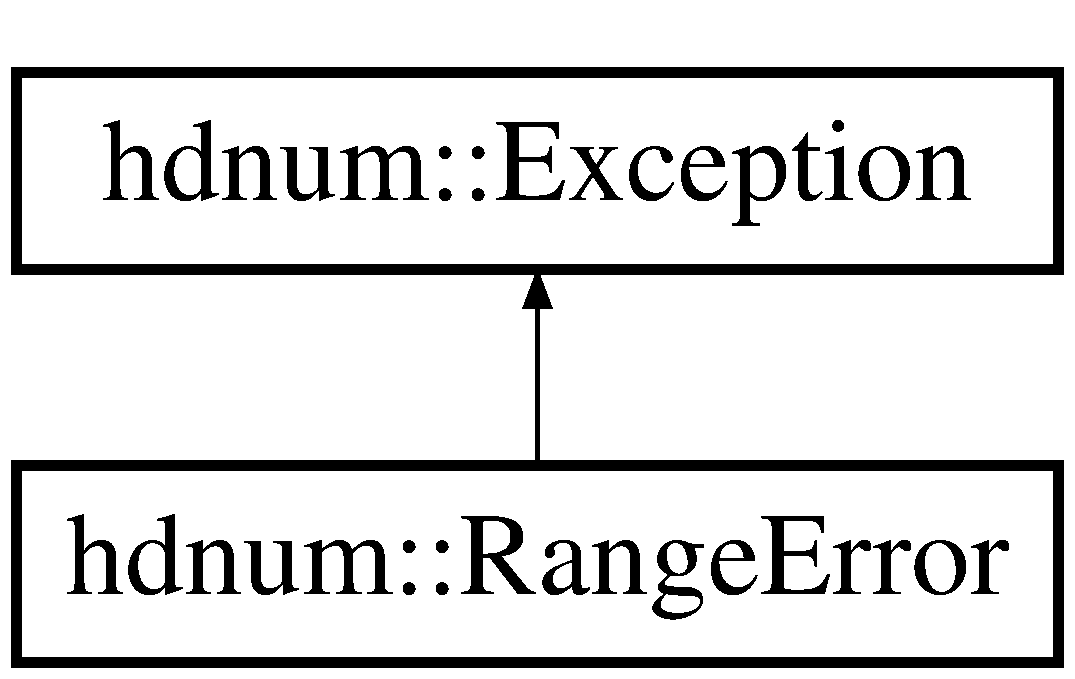
\includegraphics[height=2cm]{classhdnum_1_1RangeError}
\end{center}
\end{figure}


\subsection{Detailed Description}
Default exception class for range errors. This is the superclass for all errors which are caused because the user tries to access data that was not allocated before. These can be problems like


\begin{DoxyItemize}
\item accessing array entries behind the last entry
\item adding the fourth non zero entry in a sparse matrix with only three non zero entries per row 
\end{DoxyItemize}

The documentation for this class was generated from the following file:\begin{DoxyCompactItemize}
\item 
src/\hyperlink{exceptions_8hh}{exceptions.hh}\end{DoxyCompactItemize}

\hypertarget{classhdnum_1_1RE}{
\section{hdnum::RE$<$ M, S $>$ Class Template Reference}
\label{classhdnum_1_1RE}\index{hdnum::RE@{hdnum::RE}}
}


Adaptive one-\/step method using Richardson extrapolation.  




{\ttfamily \#include $<$ode.hh$>$}

\subsection*{Public Types}
\begin{DoxyCompactItemize}
\item 
\hypertarget{classhdnum_1_1RE_ac69dd564f38accecac013e6fdfea00e1}{
typedef M::size\_\-type \hyperlink{classhdnum_1_1RE_ac69dd564f38accecac013e6fdfea00e1}{size\_\-type}}
\label{classhdnum_1_1RE_ac69dd564f38accecac013e6fdfea00e1}

\begin{DoxyCompactList}\small\item\em export size\_\-type \item\end{DoxyCompactList}\item 
\hypertarget{classhdnum_1_1RE_ae91da4bd459d3c8961c678e9ea53cdc7}{
typedef M::time\_\-type \hyperlink{classhdnum_1_1RE_ae91da4bd459d3c8961c678e9ea53cdc7}{time\_\-type}}
\label{classhdnum_1_1RE_ae91da4bd459d3c8961c678e9ea53cdc7}

\begin{DoxyCompactList}\small\item\em export time\_\-type \item\end{DoxyCompactList}\item 
\hypertarget{classhdnum_1_1RE_a0223c61d464ed8b6fd3e84878e1b6cec}{
typedef M::number\_\-type \hyperlink{classhdnum_1_1RE_a0223c61d464ed8b6fd3e84878e1b6cec}{number\_\-type}}
\label{classhdnum_1_1RE_a0223c61d464ed8b6fd3e84878e1b6cec}

\begin{DoxyCompactList}\small\item\em export number\_\-type \item\end{DoxyCompactList}\end{DoxyCompactItemize}
\subsection*{Public Member Functions}
\begin{DoxyCompactItemize}
\item 
\hypertarget{classhdnum_1_1RE_a32795cf679545f00cb1d750cee95d168}{
\hyperlink{classhdnum_1_1RE_a32795cf679545f00cb1d750cee95d168}{RE} (const M \&model\_\-, S \&solver\_\-)}
\label{classhdnum_1_1RE_a32795cf679545f00cb1d750cee95d168}

\begin{DoxyCompactList}\small\item\em constructor stores reference to the model \item\end{DoxyCompactList}\item 
\hypertarget{classhdnum_1_1RE_aa08735eb2e917aaab79b516a89f40c97}{
void \hyperlink{classhdnum_1_1RE_aa08735eb2e917aaab79b516a89f40c97}{set\_\-dt} (\hyperlink{classhdnum_1_1RE_ae91da4bd459d3c8961c678e9ea53cdc7}{time\_\-type} dt\_\-)}
\label{classhdnum_1_1RE_aa08735eb2e917aaab79b516a89f40c97}

\begin{DoxyCompactList}\small\item\em set time step for subsequent steps \item\end{DoxyCompactList}\item 
\hypertarget{classhdnum_1_1RE_a784627ea3d588d5ba0838832db4d2856}{
void \hyperlink{classhdnum_1_1RE_a784627ea3d588d5ba0838832db4d2856}{set\_\-TOL} (\hyperlink{classhdnum_1_1RE_ae91da4bd459d3c8961c678e9ea53cdc7}{time\_\-type} TOL\_\-)}
\label{classhdnum_1_1RE_a784627ea3d588d5ba0838832db4d2856}

\begin{DoxyCompactList}\small\item\em set tolerance for adaptive computation \item\end{DoxyCompactList}\item 
\hypertarget{classhdnum_1_1RE_a65c8908666fbe5773417155ec3fc5161}{
void \hyperlink{classhdnum_1_1RE_a65c8908666fbe5773417155ec3fc5161}{step} ()}
\label{classhdnum_1_1RE_a65c8908666fbe5773417155ec3fc5161}

\begin{DoxyCompactList}\small\item\em do one step \item\end{DoxyCompactList}\item 
\hypertarget{classhdnum_1_1RE_a96ab38554c88dd93dcad6e64def6706b}{
const \hyperlink{classhdnum_1_1Vector}{Vector}$<$ \hyperlink{classhdnum_1_1RE_a0223c61d464ed8b6fd3e84878e1b6cec}{number\_\-type} $>$ \& \hyperlink{classhdnum_1_1RE_a96ab38554c88dd93dcad6e64def6706b}{get\_\-state} () const }
\label{classhdnum_1_1RE_a96ab38554c88dd93dcad6e64def6706b}

\begin{DoxyCompactList}\small\item\em get current state \item\end{DoxyCompactList}\item 
\hypertarget{classhdnum_1_1RE_a81197d3660de7de56d85aa0f880ec9fa}{
\hyperlink{classhdnum_1_1RE_ae91da4bd459d3c8961c678e9ea53cdc7}{time\_\-type} \hyperlink{classhdnum_1_1RE_a81197d3660de7de56d85aa0f880ec9fa}{get\_\-time} () const }
\label{classhdnum_1_1RE_a81197d3660de7de56d85aa0f880ec9fa}

\begin{DoxyCompactList}\small\item\em get current time \item\end{DoxyCompactList}\item 
\hypertarget{classhdnum_1_1RE_a7083da825790713eaa4bd69f179924f9}{
\hyperlink{classhdnum_1_1RE_ae91da4bd459d3c8961c678e9ea53cdc7}{time\_\-type} \hyperlink{classhdnum_1_1RE_a7083da825790713eaa4bd69f179924f9}{get\_\-dt} () const }
\label{classhdnum_1_1RE_a7083da825790713eaa4bd69f179924f9}

\begin{DoxyCompactList}\small\item\em get dt used in last step (i.e. to compute current state) \item\end{DoxyCompactList}\item 
\hypertarget{classhdnum_1_1RE_a2eb79a70aef12f55b4aa34e09f4b8ad1}{
\hyperlink{classhdnum_1_1RE_ac69dd564f38accecac013e6fdfea00e1}{size\_\-type} \hyperlink{classhdnum_1_1RE_a2eb79a70aef12f55b4aa34e09f4b8ad1}{get\_\-order} () const }
\label{classhdnum_1_1RE_a2eb79a70aef12f55b4aa34e09f4b8ad1}

\begin{DoxyCompactList}\small\item\em return consistency order of the method \item\end{DoxyCompactList}\item 
\hypertarget{classhdnum_1_1RE_aae44debd78eaf94003a076920444f79b}{
void \hyperlink{classhdnum_1_1RE_aae44debd78eaf94003a076920444f79b}{get\_\-info} () const }
\label{classhdnum_1_1RE_aae44debd78eaf94003a076920444f79b}

\begin{DoxyCompactList}\small\item\em print some information \item\end{DoxyCompactList}\end{DoxyCompactItemize}


\subsection{Detailed Description}
\subsubsection*{template$<$class M, class S$>$ class hdnum::RE$<$ M, S $>$}

Adaptive one-\/step method using Richardson extrapolation. 
\begin{DoxyTemplParams}{Template Parameters}
\item[{\em M}]a model \item[{\em S}]any of the (non-\/adaptive) one step methods (solving model M) \end{DoxyTemplParams}


The documentation for this class was generated from the following file:\begin{DoxyCompactItemize}
\item 
src/\hyperlink{ode_8hh}{ode.hh}\end{DoxyCompactItemize}

\hypertarget{classhdnum_1_1RKF45}{
\section{hdnum::RKF45$<$ M $>$ Class Template Reference}
\label{classhdnum_1_1RKF45}\index{hdnum::RKF45@{hdnum::RKF45}}
}


Adaptive Runge-\/Kutta-\/Fehlberg method.  




{\ttfamily \#include $<$ode.hh$>$}

\subsection*{Public Types}
\begin{DoxyCompactItemize}
\item 
\hypertarget{classhdnum_1_1RKF45_a7fd97c231601ffb9373fbb5dad8a60f3}{
typedef M::size\_\-type \hyperlink{classhdnum_1_1RKF45_a7fd97c231601ffb9373fbb5dad8a60f3}{size\_\-type}}
\label{classhdnum_1_1RKF45_a7fd97c231601ffb9373fbb5dad8a60f3}

\begin{DoxyCompactList}\small\item\em export size\_\-type \item\end{DoxyCompactList}\item 
\hypertarget{classhdnum_1_1RKF45_a27ab73a7d7756f59d4422a96afd9ea00}{
typedef M::time\_\-type \hyperlink{classhdnum_1_1RKF45_a27ab73a7d7756f59d4422a96afd9ea00}{time\_\-type}}
\label{classhdnum_1_1RKF45_a27ab73a7d7756f59d4422a96afd9ea00}

\begin{DoxyCompactList}\small\item\em export time\_\-type \item\end{DoxyCompactList}\item 
\hypertarget{classhdnum_1_1RKF45_af34f11a4cdc46bb0323db78fcb3712da}{
typedef M::number\_\-type \hyperlink{classhdnum_1_1RKF45_af34f11a4cdc46bb0323db78fcb3712da}{number\_\-type}}
\label{classhdnum_1_1RKF45_af34f11a4cdc46bb0323db78fcb3712da}

\begin{DoxyCompactList}\small\item\em export number\_\-type \item\end{DoxyCompactList}\end{DoxyCompactItemize}
\subsection*{Public Member Functions}
\begin{DoxyCompactItemize}
\item 
\hypertarget{classhdnum_1_1RKF45_a7757b93351fc2a2a98fe503ef92dbe3b}{
\hyperlink{classhdnum_1_1RKF45_a7757b93351fc2a2a98fe503ef92dbe3b}{RKF45} (const M \&model\_\-)}
\label{classhdnum_1_1RKF45_a7757b93351fc2a2a98fe503ef92dbe3b}

\begin{DoxyCompactList}\small\item\em constructor stores reference to the model \item\end{DoxyCompactList}\item 
\hypertarget{classhdnum_1_1RKF45_aa0724f83cd7bb44451e21b1780b3f100}{
void \hyperlink{classhdnum_1_1RKF45_aa0724f83cd7bb44451e21b1780b3f100}{set\_\-dt} (\hyperlink{classhdnum_1_1RKF45_a27ab73a7d7756f59d4422a96afd9ea00}{time\_\-type} dt\_\-)}
\label{classhdnum_1_1RKF45_aa0724f83cd7bb44451e21b1780b3f100}

\begin{DoxyCompactList}\small\item\em set time step for subsequent steps \item\end{DoxyCompactList}\item 
\hypertarget{classhdnum_1_1RKF45_ac5c815988db76d77a28e1833dd6a6cb6}{
void \hyperlink{classhdnum_1_1RKF45_ac5c815988db76d77a28e1833dd6a6cb6}{set\_\-TOL} (\hyperlink{classhdnum_1_1RKF45_a27ab73a7d7756f59d4422a96afd9ea00}{time\_\-type} TOL\_\-)}
\label{classhdnum_1_1RKF45_ac5c815988db76d77a28e1833dd6a6cb6}

\begin{DoxyCompactList}\small\item\em set tolerance for adaptive computation \item\end{DoxyCompactList}\item 
\hypertarget{classhdnum_1_1RKF45_aa61bd540faf3b35e42788e5127a2ecf1}{
void \hyperlink{classhdnum_1_1RKF45_aa61bd540faf3b35e42788e5127a2ecf1}{step} ()}
\label{classhdnum_1_1RKF45_aa61bd540faf3b35e42788e5127a2ecf1}

\begin{DoxyCompactList}\small\item\em do one step \item\end{DoxyCompactList}\item 
\hypertarget{classhdnum_1_1RKF45_a13ea82e111ab9e30fd9b6faf5e825e3d}{
const \hyperlink{classhdnum_1_1Vector}{Vector}$<$ \hyperlink{classhdnum_1_1RKF45_af34f11a4cdc46bb0323db78fcb3712da}{number\_\-type} $>$ \& \hyperlink{classhdnum_1_1RKF45_a13ea82e111ab9e30fd9b6faf5e825e3d}{get\_\-state} () const }
\label{classhdnum_1_1RKF45_a13ea82e111ab9e30fd9b6faf5e825e3d}

\begin{DoxyCompactList}\small\item\em get current state \item\end{DoxyCompactList}\item 
\hypertarget{classhdnum_1_1RKF45_a5f9dfeeba9abeee37fdc5e8d79d30488}{
\hyperlink{classhdnum_1_1RKF45_a27ab73a7d7756f59d4422a96afd9ea00}{time\_\-type} \hyperlink{classhdnum_1_1RKF45_a5f9dfeeba9abeee37fdc5e8d79d30488}{get\_\-time} () const }
\label{classhdnum_1_1RKF45_a5f9dfeeba9abeee37fdc5e8d79d30488}

\begin{DoxyCompactList}\small\item\em get current time \item\end{DoxyCompactList}\item 
\hypertarget{classhdnum_1_1RKF45_aee7cdf5b333ca31418917f76ab70dcef}{
\hyperlink{classhdnum_1_1RKF45_a27ab73a7d7756f59d4422a96afd9ea00}{time\_\-type} \hyperlink{classhdnum_1_1RKF45_aee7cdf5b333ca31418917f76ab70dcef}{get\_\-dt} () const }
\label{classhdnum_1_1RKF45_aee7cdf5b333ca31418917f76ab70dcef}

\begin{DoxyCompactList}\small\item\em get dt used in last step (i.e. to compute current state) \item\end{DoxyCompactList}\item 
\hypertarget{classhdnum_1_1RKF45_ace56b907855d8323b4161ebc3e3d20dc}{
\hyperlink{classhdnum_1_1RKF45_a7fd97c231601ffb9373fbb5dad8a60f3}{size\_\-type} \hyperlink{classhdnum_1_1RKF45_ace56b907855d8323b4161ebc3e3d20dc}{get\_\-order} () const }
\label{classhdnum_1_1RKF45_ace56b907855d8323b4161ebc3e3d20dc}

\begin{DoxyCompactList}\small\item\em return consistency order of the method \item\end{DoxyCompactList}\item 
\hypertarget{classhdnum_1_1RKF45_af3f56f53dc2398a808e4fa85c658c56c}{
void \hyperlink{classhdnum_1_1RKF45_af3f56f53dc2398a808e4fa85c658c56c}{get\_\-info} () const }
\label{classhdnum_1_1RKF45_af3f56f53dc2398a808e4fa85c658c56c}

\begin{DoxyCompactList}\small\item\em print some information \item\end{DoxyCompactList}\end{DoxyCompactItemize}


\subsection{Detailed Description}
\subsubsection*{template$<$class M$>$ class hdnum::RKF45$<$ M $>$}

Adaptive Runge-\/Kutta-\/Fehlberg method. 
\begin{DoxyTemplParams}{Template Parameters}
\item[{\em M}]the model type \end{DoxyTemplParams}


The documentation for this class was generated from the following file:\begin{DoxyCompactItemize}
\item 
src/\hyperlink{ode_8hh}{ode.hh}\end{DoxyCompactItemize}

\hypertarget{classhdnum_1_1RungeKutta4}{
\section{hdnum::RungeKutta4$<$ M $>$ Class Template Reference}
\label{classhdnum_1_1RungeKutta4}\index{hdnum::RungeKutta4@{hdnum::RungeKutta4}}
}


classical Runge-\/Kutta method (order 4 with 4 stages)  




{\ttfamily \#include $<$ode.hh$>$}

\subsection*{Public Types}
\begin{DoxyCompactItemize}
\item 
\hypertarget{classhdnum_1_1RungeKutta4_a35c0f2a31327913676b7287fb1ef23dc}{
typedef M::size\_\-type \hyperlink{classhdnum_1_1RungeKutta4_a35c0f2a31327913676b7287fb1ef23dc}{size\_\-type}}
\label{classhdnum_1_1RungeKutta4_a35c0f2a31327913676b7287fb1ef23dc}

\begin{DoxyCompactList}\small\item\em export size\_\-type \item\end{DoxyCompactList}\item 
\hypertarget{classhdnum_1_1RungeKutta4_accd5f055f7a407e0012622fbf4298e84}{
typedef M::time\_\-type \hyperlink{classhdnum_1_1RungeKutta4_accd5f055f7a407e0012622fbf4298e84}{time\_\-type}}
\label{classhdnum_1_1RungeKutta4_accd5f055f7a407e0012622fbf4298e84}

\begin{DoxyCompactList}\small\item\em export time\_\-type \item\end{DoxyCompactList}\item 
\hypertarget{classhdnum_1_1RungeKutta4_a8a2af290f6503769876570bba58fdff2}{
typedef M::number\_\-type \hyperlink{classhdnum_1_1RungeKutta4_a8a2af290f6503769876570bba58fdff2}{number\_\-type}}
\label{classhdnum_1_1RungeKutta4_a8a2af290f6503769876570bba58fdff2}

\begin{DoxyCompactList}\small\item\em export number\_\-type \item\end{DoxyCompactList}\end{DoxyCompactItemize}
\subsection*{Public Member Functions}
\begin{DoxyCompactItemize}
\item 
\hypertarget{classhdnum_1_1RungeKutta4_a576f1d99c638594c745b54956254c100}{
\hyperlink{classhdnum_1_1RungeKutta4_a576f1d99c638594c745b54956254c100}{RungeKutta4} (const M \&model\_\-)}
\label{classhdnum_1_1RungeKutta4_a576f1d99c638594c745b54956254c100}

\begin{DoxyCompactList}\small\item\em constructor stores reference to the model \item\end{DoxyCompactList}\item 
\hypertarget{classhdnum_1_1RungeKutta4_a035f34c6ac918a9ae8f0fd2bc67da620}{
void \hyperlink{classhdnum_1_1RungeKutta4_a035f34c6ac918a9ae8f0fd2bc67da620}{set\_\-dt} (\hyperlink{classhdnum_1_1RungeKutta4_accd5f055f7a407e0012622fbf4298e84}{time\_\-type} dt\_\-)}
\label{classhdnum_1_1RungeKutta4_a035f34c6ac918a9ae8f0fd2bc67da620}

\begin{DoxyCompactList}\small\item\em set time step for subsequent steps \item\end{DoxyCompactList}\item 
\hypertarget{classhdnum_1_1RungeKutta4_a243e063d6c0a8982a4addc1d97f547e0}{
void \hyperlink{classhdnum_1_1RungeKutta4_a243e063d6c0a8982a4addc1d97f547e0}{step} ()}
\label{classhdnum_1_1RungeKutta4_a243e063d6c0a8982a4addc1d97f547e0}

\begin{DoxyCompactList}\small\item\em do one step \item\end{DoxyCompactList}\item 
\hypertarget{classhdnum_1_1RungeKutta4_a06f337a2c23a40ea1cb798365879c9aa}{
void \hyperlink{classhdnum_1_1RungeKutta4_a06f337a2c23a40ea1cb798365879c9aa}{set\_\-state} (\hyperlink{classhdnum_1_1RungeKutta4_accd5f055f7a407e0012622fbf4298e84}{time\_\-type} t\_\-, const \hyperlink{classhdnum_1_1Vector}{Vector}$<$ \hyperlink{classhdnum_1_1RungeKutta4_a8a2af290f6503769876570bba58fdff2}{number\_\-type} $>$ \&u\_\-)}
\label{classhdnum_1_1RungeKutta4_a06f337a2c23a40ea1cb798365879c9aa}

\begin{DoxyCompactList}\small\item\em set current state \item\end{DoxyCompactList}\item 
\hypertarget{classhdnum_1_1RungeKutta4_a2769ffd570ccb23004b4996a4cebf279}{
const \hyperlink{classhdnum_1_1Vector}{Vector}$<$ \hyperlink{classhdnum_1_1RungeKutta4_a8a2af290f6503769876570bba58fdff2}{number\_\-type} $>$ \& \hyperlink{classhdnum_1_1RungeKutta4_a2769ffd570ccb23004b4996a4cebf279}{get\_\-state} () const }
\label{classhdnum_1_1RungeKutta4_a2769ffd570ccb23004b4996a4cebf279}

\begin{DoxyCompactList}\small\item\em get current state \item\end{DoxyCompactList}\item 
\hypertarget{classhdnum_1_1RungeKutta4_a371015562c4918d748b49df3c521b0d0}{
\hyperlink{classhdnum_1_1RungeKutta4_accd5f055f7a407e0012622fbf4298e84}{time\_\-type} \hyperlink{classhdnum_1_1RungeKutta4_a371015562c4918d748b49df3c521b0d0}{get\_\-time} () const }
\label{classhdnum_1_1RungeKutta4_a371015562c4918d748b49df3c521b0d0}

\begin{DoxyCompactList}\small\item\em get current time \item\end{DoxyCompactList}\item 
\hypertarget{classhdnum_1_1RungeKutta4_aa808a6a3dfd672359999e44906da4692}{
\hyperlink{classhdnum_1_1RungeKutta4_accd5f055f7a407e0012622fbf4298e84}{time\_\-type} \hyperlink{classhdnum_1_1RungeKutta4_aa808a6a3dfd672359999e44906da4692}{get\_\-dt} () const }
\label{classhdnum_1_1RungeKutta4_aa808a6a3dfd672359999e44906da4692}

\begin{DoxyCompactList}\small\item\em get dt used in last step (i.e. to compute current state) \item\end{DoxyCompactList}\item 
\hypertarget{classhdnum_1_1RungeKutta4_a74544dbe43813719b549d97903772a52}{
\hyperlink{classhdnum_1_1RungeKutta4_a35c0f2a31327913676b7287fb1ef23dc}{size\_\-type} \hyperlink{classhdnum_1_1RungeKutta4_a74544dbe43813719b549d97903772a52}{get\_\-order} () const }
\label{classhdnum_1_1RungeKutta4_a74544dbe43813719b549d97903772a52}

\begin{DoxyCompactList}\small\item\em return consistency order of the method \item\end{DoxyCompactList}\end{DoxyCompactItemize}


\subsection{Detailed Description}
\subsubsection*{template$<$class M$>$ class hdnum::RungeKutta4$<$ M $>$}

classical Runge-\/Kutta method (order 4 with 4 stages) The ODE solver is parametrized by a model. The model also exports all relevant types for time and states. The ODE solver encapsulates the states needed for the computation.


\begin{DoxyTemplParams}{Template Parameters}
\item[{\em M}]the model type \end{DoxyTemplParams}


The documentation for this class was generated from the following file:\begin{DoxyCompactItemize}
\item 
src/\hyperlink{ode_8hh}{ode.hh}\end{DoxyCompactItemize}

\hypertarget{classhdnum_1_1SGrid}{
\section{hdnum::SGrid$<$ N, DF, dimension $>$ Class Template Reference}
\label{classhdnum_1_1SGrid}\index{hdnum::SGrid@{hdnum::SGrid}}
}


Structured Grid for Finite Differences.  




{\ttfamily \#include $<$sgrid.hh$>$}

\subsection*{Public Types}
\begin{DoxyCompactItemize}
\item 
enum \{ {\bfseries dim} =  dimension
 \}
\item 
\hypertarget{classhdnum_1_1SGrid_aba7c973b280ecd56f211ac4b8d746280}{
typedef std::size\_\-t \hyperlink{classhdnum_1_1SGrid_aba7c973b280ecd56f211ac4b8d746280}{size\_\-type}}
\label{classhdnum_1_1SGrid_aba7c973b280ecd56f211ac4b8d746280}

\begin{DoxyCompactList}\small\item\em Export size type. \item\end{DoxyCompactList}\item 
\hypertarget{classhdnum_1_1SGrid_ab27de1dac2771512d96a858153db82f5}{
typedef N \hyperlink{classhdnum_1_1SGrid_ab27de1dac2771512d96a858153db82f5}{number\_\-type}}
\label{classhdnum_1_1SGrid_ab27de1dac2771512d96a858153db82f5}

\begin{DoxyCompactList}\small\item\em Export number type. \item\end{DoxyCompactList}\item 
\hypertarget{classhdnum_1_1SGrid_a0442a89c48bb466449cb1a7e5d4cc5f6}{
typedef DF \hyperlink{classhdnum_1_1SGrid_a0442a89c48bb466449cb1a7e5d4cc5f6}{DomainFunction}}
\label{classhdnum_1_1SGrid_a0442a89c48bb466449cb1a7e5d4cc5f6}

\begin{DoxyCompactList}\small\item\em Type of the function defining the domain. \item\end{DoxyCompactList}\end{DoxyCompactItemize}
\subsection*{Public Member Functions}
\begin{DoxyCompactItemize}
\item 
\hyperlink{classhdnum_1_1SGrid_ada654dda6b112ebe8c29fef72f917b7b}{SGrid} (const \hyperlink{classhdnum_1_1Vector}{Vector}$<$ \hyperlink{classhdnum_1_1SGrid_ab27de1dac2771512d96a858153db82f5}{number\_\-type} $>$ extent\_\-, const \hyperlink{classhdnum_1_1Vector}{Vector}$<$ \hyperlink{classhdnum_1_1SGrid_aba7c973b280ecd56f211ac4b8d746280}{size\_\-type} $>$ size\_\-, const \hyperlink{classhdnum_1_1SGrid_a0442a89c48bb466449cb1a7e5d4cc5f6}{DomainFunction} \&df\_\-)
\begin{DoxyCompactList}\small\item\em Constructor. \item\end{DoxyCompactList}\item 
\hyperlink{classhdnum_1_1SGrid_aba7c973b280ecd56f211ac4b8d746280}{size\_\-type} \hyperlink{classhdnum_1_1SGrid_a64eff228d60e47b1ecceaf331ba54173}{getNeighborIndex} (const \hyperlink{classhdnum_1_1SGrid_aba7c973b280ecd56f211ac4b8d746280}{size\_\-type} ln, const \hyperlink{classhdnum_1_1SGrid_aba7c973b280ecd56f211ac4b8d746280}{size\_\-type} n\_\-dim, const int n\_\-side, const int k=1) const 
\begin{DoxyCompactList}\small\item\em Provides the index of the k-\/th neighbor of the node with index ln. \item\end{DoxyCompactList}\item 
\hypertarget{classhdnum_1_1SGrid_a47cc9aa07b061592f69480c0d128e70c}{
bool \hyperlink{classhdnum_1_1SGrid_a47cc9aa07b061592f69480c0d128e70c}{isBoundaryNode} (const \hyperlink{classhdnum_1_1SGrid_aba7c973b280ecd56f211ac4b8d746280}{size\_\-type} ln) const }
\label{classhdnum_1_1SGrid_a47cc9aa07b061592f69480c0d128e70c}

\begin{DoxyCompactList}\small\item\em Returns true if the node is on the boundary of the discrete compuational domain. \item\end{DoxyCompactList}\item 
\hypertarget{classhdnum_1_1SGrid_a60ed482ea236e8fe974401e637efd526}{
\hyperlink{classhdnum_1_1SGrid_aba7c973b280ecd56f211ac4b8d746280}{size\_\-type} \hyperlink{classhdnum_1_1SGrid_a60ed482ea236e8fe974401e637efd526}{getNumberOfNodes} () const }
\label{classhdnum_1_1SGrid_a60ed482ea236e8fe974401e637efd526}

\begin{DoxyCompactList}\small\item\em Returns the number of nodes which are in the compuational domain. \item\end{DoxyCompactList}\item 
\hypertarget{classhdnum_1_1SGrid_a3f45476d2463aa8ee9d7cb3c2fc13e86}{
\hyperlink{classhdnum_1_1Vector}{Vector}$<$ \hyperlink{classhdnum_1_1SGrid_aba7c973b280ecd56f211ac4b8d746280}{size\_\-type} $>$ {\bfseries getGridSize} () const }
\label{classhdnum_1_1SGrid_a3f45476d2463aa8ee9d7cb3c2fc13e86}

\item 
\hypertarget{classhdnum_1_1SGrid_af77f316487e41dc0f7bcd972f2c12a85}{
\hyperlink{classhdnum_1_1Vector}{Vector}$<$ \hyperlink{classhdnum_1_1SGrid_ab27de1dac2771512d96a858153db82f5}{number\_\-type} $>$ \hyperlink{classhdnum_1_1SGrid_af77f316487e41dc0f7bcd972f2c12a85}{getCellWidth} () const }
\label{classhdnum_1_1SGrid_af77f316487e41dc0f7bcd972f2c12a85}

\begin{DoxyCompactList}\small\item\em Returns the cell width h of the structured grid. \item\end{DoxyCompactList}\item 
\hypertarget{classhdnum_1_1SGrid_a3d5abab14a7aea4304ebf01a0567c733}{
\hyperlink{classhdnum_1_1Vector}{Vector}$<$ \hyperlink{classhdnum_1_1SGrid_ab27de1dac2771512d96a858153db82f5}{number\_\-type} $>$ \hyperlink{classhdnum_1_1SGrid_a3d5abab14a7aea4304ebf01a0567c733}{getCoordinates} (const \hyperlink{classhdnum_1_1SGrid_aba7c973b280ecd56f211ac4b8d746280}{size\_\-type} ln) const }
\label{classhdnum_1_1SGrid_a3d5abab14a7aea4304ebf01a0567c733}

\begin{DoxyCompactList}\small\item\em Returns the world coordinates of the node with the given node index. \item\end{DoxyCompactList}\item 
\hypertarget{classhdnum_1_1SGrid_a136c4dcd9ff0fd17f4c590ce3334e05f}{
std::vector$<$ \hyperlink{classhdnum_1_1Vector}{Vector}$<$ \hyperlink{classhdnum_1_1SGrid_ab27de1dac2771512d96a858153db82f5}{number\_\-type} $>$ $>$ {\bfseries getNodeCoordinates} () const }
\label{classhdnum_1_1SGrid_a136c4dcd9ff0fd17f4c590ce3334e05f}

\end{DoxyCompactItemize}
\subsection*{Public Attributes}
\begin{DoxyCompactItemize}
\item 
\hypertarget{classhdnum_1_1SGrid_aedaa35a3ac460551ba71aabebf411b5d}{
const \hyperlink{classhdnum_1_1SGrid_aba7c973b280ecd56f211ac4b8d746280}{size\_\-type} \hyperlink{classhdnum_1_1SGrid_aedaa35a3ac460551ba71aabebf411b5d}{invalid\_\-node}}
\label{classhdnum_1_1SGrid_aedaa35a3ac460551ba71aabebf411b5d}

\begin{DoxyCompactList}\small\item\em The value which is returned to indicate an invalid node. \item\end{DoxyCompactList}\end{DoxyCompactItemize}
\subsection*{Static Public Attributes}
\begin{DoxyCompactItemize}
\item 
\hypertarget{classhdnum_1_1SGrid_a0824662b4e8828f13b1600a4226e82a0}{
static const int \hyperlink{classhdnum_1_1SGrid_a0824662b4e8828f13b1600a4226e82a0}{positive} = 1}
\label{classhdnum_1_1SGrid_a0824662b4e8828f13b1600a4226e82a0}

\begin{DoxyCompactList}\small\item\em Side definitions for usage in getNeighborIndex(..). \item\end{DoxyCompactList}\item 
\hypertarget{classhdnum_1_1SGrid_a4e9a18163df1318fc15ac094ac28196b}{
static const int {\bfseries negative} = -\/1}
\label{classhdnum_1_1SGrid_a4e9a18163df1318fc15ac094ac28196b}

\end{DoxyCompactItemize}


\subsection{Detailed Description}
\subsubsection*{template$<$class N, class DF, int dimension$>$ class hdnum::SGrid$<$ N, DF, dimension $>$}

Structured Grid for Finite Differences. 
\begin{DoxyTemplParams}{Template Parameters}
\item[{\em N}]A continuous type representing coordinate values. \item[{\em DF}]A boolean function which defines the domain. \item[{\em dimension}]The grid dimension. \end{DoxyTemplParams}


\subsection{Constructor \& Destructor Documentation}
\hypertarget{classhdnum_1_1SGrid_ada654dda6b112ebe8c29fef72f917b7b}{
\index{hdnum::SGrid@{hdnum::SGrid}!SGrid@{SGrid}}
\index{SGrid@{SGrid}!hdnum::SGrid@{hdnum::SGrid}}
\subsubsection[{SGrid}]{\setlength{\rightskip}{0pt plus 5cm}template$<$class N , class DF , int dimension$>$ {\bf hdnum::SGrid}$<$ N, DF, dimension $>$::{\bf SGrid} (const {\bf Vector}$<$ {\bf number\_\-type} $>$ {\em extent\_\-}, \/  const {\bf Vector}$<$ {\bf size\_\-type} $>$ {\em size\_\-}, \/  const {\bf DomainFunction} \& {\em df\_\-})\hspace{0.3cm}{\ttfamily  \mbox{[}inline\mbox{]}}}}
\label{classhdnum_1_1SGrid_ada654dda6b112ebe8c29fef72f917b7b}


Constructor. 


\begin{DoxyParams}{Parameters}
\item[\mbox{$\leftarrow$} {\em extent\_\-}]The extent of the grid domain. The actual computational domain may be smaller and is defined by the domain function df\_\-.\item[\mbox{$\leftarrow$} {\em size\_\-}]The number of nodes in each grid dimension.\item[\mbox{$\leftarrow$} {\em df\_\-}]The domain function. It has to provide a boolean function evaluate(Vector$<$number\_\-type$>$ x) which returns true if the node which is positioned at the coordinates of x is within the computational domain. \end{DoxyParams}


\subsection{Member Function Documentation}
\hypertarget{classhdnum_1_1SGrid_a64eff228d60e47b1ecceaf331ba54173}{
\index{hdnum::SGrid@{hdnum::SGrid}!getNeighborIndex@{getNeighborIndex}}
\index{getNeighborIndex@{getNeighborIndex}!hdnum::SGrid@{hdnum::SGrid}}
\subsubsection[{getNeighborIndex}]{\setlength{\rightskip}{0pt plus 5cm}template$<$class N , class DF , int dimension$>$ {\bf size\_\-type} {\bf hdnum::SGrid}$<$ N, DF, dimension $>$::getNeighborIndex (const {\bf size\_\-type} {\em ln}, \/  const {\bf size\_\-type} {\em n\_\-dim}, \/  const int {\em n\_\-side}, \/  const int {\em k} = {\ttfamily 1}) const\hspace{0.3cm}{\ttfamily  \mbox{[}inline\mbox{]}}}}
\label{classhdnum_1_1SGrid_a64eff228d60e47b1ecceaf331ba54173}


Provides the index of the k-\/th neighbor of the node with index ln. 


\begin{DoxyParams}{Parameters}
\item[\mbox{$\leftarrow$} {\em ln}]Index of the node whose neighbor is to be determined.\item[\mbox{$\leftarrow$} {\em n\_\-dim}]The axes which connects the node and its neighbor (e.g. n\_\-dim = 0 for a neighbor in the direction of the x-\/axes\item[\mbox{$\leftarrow$} {\em n\_\-side}]Determines whether the neighbor is in positive of negative direction of the given axes. Should be either \hyperlink{classhdnum_1_1SGrid_a0824662b4e8828f13b1600a4226e82a0}{SGrid::positive} or SGrid::negative .\item[\mbox{$\leftarrow$} {\em k}]For k=1 it will return the direct neighbor. Higher values will give distant nodes in the given direction. If the indicated node is not within the grid any more, then invalid\_\-node will be returned. For k=0 it will simply return ln.\end{DoxyParams}
\begin{DoxyReturn}{Returns}
size\_\-type The index of the neighbor node. 
\end{DoxyReturn}


The documentation for this class was generated from the following file:\begin{DoxyCompactItemize}
\item 
src/sgrid.hh\end{DoxyCompactItemize}

\hypertarget{classhdnum_1_1SquareRootProblem}{
\section{hdnum::SquareRootProblem$<$ N $>$ Class Template Reference}
\label{classhdnum_1_1SquareRootProblem}\index{hdnum::SquareRootProblem@{hdnum::SquareRootProblem}}
}


Example class for a nonlinear model F(x) = 0;.  




{\ttfamily \#include $<$newton.hh$>$}

\subsection*{Public Types}
\begin{DoxyCompactItemize}
\item 
\hypertarget{classhdnum_1_1SquareRootProblem_a9c7024d33b3c33be60fd50cf8a95ec12}{
typedef std::size\_\-t \hyperlink{classhdnum_1_1SquareRootProblem_a9c7024d33b3c33be60fd50cf8a95ec12}{size\_\-type}}
\label{classhdnum_1_1SquareRootProblem_a9c7024d33b3c33be60fd50cf8a95ec12}

\begin{DoxyCompactList}\small\item\em export size\_\-type \item\end{DoxyCompactList}\item 
\hypertarget{classhdnum_1_1SquareRootProblem_a2aada07411c6a24edd9183c73b79f042}{
typedef N \hyperlink{classhdnum_1_1SquareRootProblem_a2aada07411c6a24edd9183c73b79f042}{number\_\-type}}
\label{classhdnum_1_1SquareRootProblem_a2aada07411c6a24edd9183c73b79f042}

\begin{DoxyCompactList}\small\item\em export number\_\-type \item\end{DoxyCompactList}\end{DoxyCompactItemize}
\subsection*{Public Member Functions}
\begin{DoxyCompactItemize}
\item 
\hypertarget{classhdnum_1_1SquareRootProblem_a33e13342dd64285b8d1f9793c8f68193}{
\hyperlink{classhdnum_1_1SquareRootProblem_a33e13342dd64285b8d1f9793c8f68193}{SquareRootProblem} (\hyperlink{classhdnum_1_1SquareRootProblem_a2aada07411c6a24edd9183c73b79f042}{number\_\-type} a\_\-)}
\label{classhdnum_1_1SquareRootProblem_a33e13342dd64285b8d1f9793c8f68193}

\begin{DoxyCompactList}\small\item\em constructor stores parameter lambda \item\end{DoxyCompactList}\item 
\hypertarget{classhdnum_1_1SquareRootProblem_a57ef59e899224f98c7b338373df82646}{
std::size\_\-t \hyperlink{classhdnum_1_1SquareRootProblem_a57ef59e899224f98c7b338373df82646}{size} () const }
\label{classhdnum_1_1SquareRootProblem_a57ef59e899224f98c7b338373df82646}

\begin{DoxyCompactList}\small\item\em return number of componentes for the model \item\end{DoxyCompactList}\item 
\hypertarget{classhdnum_1_1SquareRootProblem_a6d8f30d61e703044b4cb84ce8ef9c479}{
void \hyperlink{classhdnum_1_1SquareRootProblem_a6d8f30d61e703044b4cb84ce8ef9c479}{F} (const \hyperlink{classhdnum_1_1Vector}{Vector}$<$ N $>$ \&x, \hyperlink{classhdnum_1_1Vector}{Vector}$<$ N $>$ \&result) const }
\label{classhdnum_1_1SquareRootProblem_a6d8f30d61e703044b4cb84ce8ef9c479}

\begin{DoxyCompactList}\small\item\em model evaluation \item\end{DoxyCompactList}\item 
\hypertarget{classhdnum_1_1SquareRootProblem_ab5a5565fde89e4794d5b819ea76b9a1e}{
void \hyperlink{classhdnum_1_1SquareRootProblem_ab5a5565fde89e4794d5b819ea76b9a1e}{F\_\-x} (const \hyperlink{classhdnum_1_1Vector}{Vector}$<$ N $>$ \&x, \hyperlink{classhdnum_1_1Matrix}{Matrix}$<$ N $>$ \&result) const }
\label{classhdnum_1_1SquareRootProblem_ab5a5565fde89e4794d5b819ea76b9a1e}

\begin{DoxyCompactList}\small\item\em jacobian evaluation needed for implicit solvers \item\end{DoxyCompactList}\end{DoxyCompactItemize}


\subsection{Detailed Description}
\subsubsection*{template$<$class N$>$ class hdnum::SquareRootProblem$<$ N $>$}

Example class for a nonlinear model F(x) = 0;. This example solves F(x) = x$\ast$x -\/ a = 0


\begin{DoxyTemplParams}{Template Parameters}
\item[{\em N}]a type representing x and F components \end{DoxyTemplParams}


The documentation for this class was generated from the following file:\begin{DoxyCompactItemize}
\item 
src/\hyperlink{newton_8hh}{newton.hh}\end{DoxyCompactItemize}

\hypertarget{classhdnum_1_1StationarySolver}{
\section{hdnum::StationarySolver$<$ M $>$ Class Template Reference}
\label{classhdnum_1_1StationarySolver}\index{hdnum::StationarySolver@{hdnum::StationarySolver}}
}


Stationary problem solver. E.g. for elliptic problmes.  




{\ttfamily \#include $<$pde.hh$>$}

\subsection*{Public Types}
\begin{DoxyCompactItemize}
\item 
\hypertarget{classhdnum_1_1StationarySolver_a95c041e1f3af75fd035bd94cb58184d8}{
typedef M::size\_\-type \hyperlink{classhdnum_1_1StationarySolver_a95c041e1f3af75fd035bd94cb58184d8}{size\_\-type}}
\label{classhdnum_1_1StationarySolver_a95c041e1f3af75fd035bd94cb58184d8}

\begin{DoxyCompactList}\small\item\em export size\_\-type \item\end{DoxyCompactList}\item 
\hypertarget{classhdnum_1_1StationarySolver_a54c185de5fd4ddd83991cf985e89f40b}{
typedef M::time\_\-type \hyperlink{classhdnum_1_1StationarySolver_a54c185de5fd4ddd83991cf985e89f40b}{time\_\-type}}
\label{classhdnum_1_1StationarySolver_a54c185de5fd4ddd83991cf985e89f40b}

\begin{DoxyCompactList}\small\item\em export time\_\-type \item\end{DoxyCompactList}\item 
\hypertarget{classhdnum_1_1StationarySolver_a48abc9e5fb531e68c63e5c72bdbb28a6}{
typedef M::number\_\-type \hyperlink{classhdnum_1_1StationarySolver_a48abc9e5fb531e68c63e5c72bdbb28a6}{number\_\-type}}
\label{classhdnum_1_1StationarySolver_a48abc9e5fb531e68c63e5c72bdbb28a6}

\begin{DoxyCompactList}\small\item\em export number\_\-type \item\end{DoxyCompactList}\end{DoxyCompactItemize}
\subsection*{Public Member Functions}
\begin{DoxyCompactItemize}
\item 
\hypertarget{classhdnum_1_1StationarySolver_a4282c63a68f76418efa5a924c34bcfc1}{
\hyperlink{classhdnum_1_1StationarySolver_a4282c63a68f76418efa5a924c34bcfc1}{StationarySolver} (const M \&model\_\-)}
\label{classhdnum_1_1StationarySolver_a4282c63a68f76418efa5a924c34bcfc1}

\begin{DoxyCompactList}\small\item\em constructor stores reference to the model \item\end{DoxyCompactList}\item 
\hypertarget{classhdnum_1_1StationarySolver_a7efb580302c52ed737346f05536b94c6}{
void \hyperlink{classhdnum_1_1StationarySolver_a7efb580302c52ed737346f05536b94c6}{solve} ()}
\label{classhdnum_1_1StationarySolver_a7efb580302c52ed737346f05536b94c6}

\begin{DoxyCompactList}\small\item\em do one step \item\end{DoxyCompactList}\item 
\hypertarget{classhdnum_1_1StationarySolver_a057916fb88d97f739ecdd00e5237297c}{
const \hyperlink{classhdnum_1_1Vector}{Vector}$<$ \hyperlink{classhdnum_1_1StationarySolver_a48abc9e5fb531e68c63e5c72bdbb28a6}{number\_\-type} $>$ \& \hyperlink{classhdnum_1_1StationarySolver_a057916fb88d97f739ecdd00e5237297c}{get\_\-state} () const }
\label{classhdnum_1_1StationarySolver_a057916fb88d97f739ecdd00e5237297c}

\begin{DoxyCompactList}\small\item\em get current state \item\end{DoxyCompactList}\item 
\hypertarget{classhdnum_1_1StationarySolver_a33ef43557b544c275e2240f155a33e6f}{
\hyperlink{classhdnum_1_1StationarySolver_a95c041e1f3af75fd035bd94cb58184d8}{size\_\-type} \hyperlink{classhdnum_1_1StationarySolver_a33ef43557b544c275e2240f155a33e6f}{get\_\-order} () const }
\label{classhdnum_1_1StationarySolver_a33ef43557b544c275e2240f155a33e6f}

\begin{DoxyCompactList}\small\item\em return consistency order of the method \item\end{DoxyCompactList}\end{DoxyCompactItemize}


\subsection{Detailed Description}
\subsubsection*{template$<$class M$>$ class hdnum::StationarySolver$<$ M $>$}

Stationary problem solver. E.g. for elliptic problmes. The PDE solver is parametrized by a model. The model also exports all relevant types for the solution. The PDE solver encapsulates the states needed for the computation.


\begin{DoxyTemplParams}{Template Parameters}
\item[{\em M}]the model type \end{DoxyTemplParams}


The documentation for this class was generated from the following file:\begin{DoxyCompactItemize}
\item 
src/\hyperlink{pde_8hh}{pde.hh}\end{DoxyCompactItemize}

\hypertarget{classhdnum_1_1SystemError}{
\section{hdnum::SystemError Class Reference}
\label{classhdnum_1_1SystemError}\index{hdnum::SystemError@{hdnum::SystemError}}
}


Default exception class for OS errors.  




{\ttfamily \#include $<$exceptions.hh$>$}

Inheritance diagram for hdnum::SystemError:\begin{figure}[H]
\begin{center}
\leavevmode
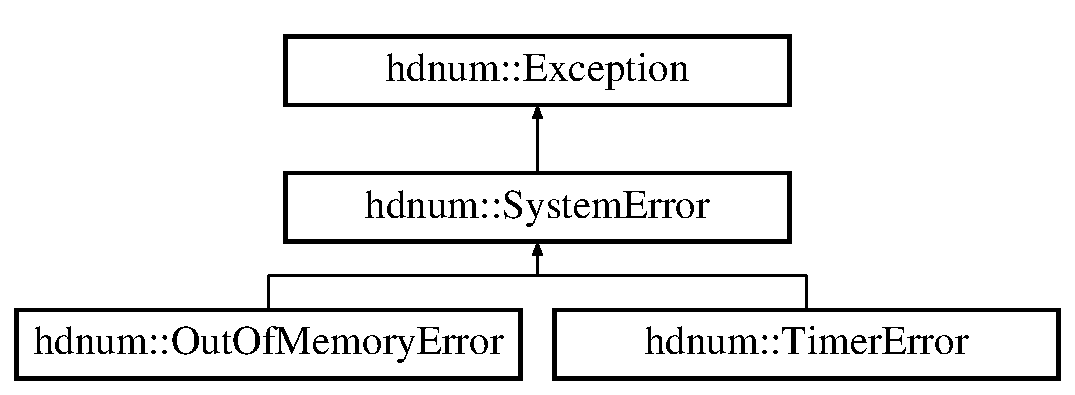
\includegraphics[height=3cm]{classhdnum_1_1SystemError}
\end{center}
\end{figure}


\subsection{Detailed Description}
Default exception class for OS errors. This class is thrown when a system-\/call is used and returns an error. 

The documentation for this class was generated from the following file:\begin{DoxyCompactItemize}
\item 
src/\hyperlink{exceptions_8hh}{exceptions.hh}\end{DoxyCompactItemize}

\hypertarget{classhdnum_1_1Timer}{
\section{hdnum::Timer Class Reference}
\label{classhdnum_1_1Timer}\index{hdnum::Timer@{hdnum::Timer}}
}


A simple stop watch.  




{\ttfamily \#include $<$timer.hh$>$}

\subsection*{Public Member Functions}
\begin{DoxyCompactItemize}
\item 
\hypertarget{classhdnum_1_1Timer_aa21efdb01cfd44867a39d6321764f368}{
\hyperlink{classhdnum_1_1Timer_aa21efdb01cfd44867a39d6321764f368}{Timer} ()  throw (TimerError)}
\label{classhdnum_1_1Timer_aa21efdb01cfd44867a39d6321764f368}

\begin{DoxyCompactList}\small\item\em A new timer, start immediately. \item\end{DoxyCompactList}\item 
\hypertarget{classhdnum_1_1Timer_ad9169c761853bd68249ce1a5d4af1511}{
void \hyperlink{classhdnum_1_1Timer_ad9169c761853bd68249ce1a5d4af1511}{reset} ()  throw (TimerError)}
\label{classhdnum_1_1Timer_ad9169c761853bd68249ce1a5d4af1511}

\begin{DoxyCompactList}\small\item\em Reset timer. \item\end{DoxyCompactList}\item 
\hypertarget{classhdnum_1_1Timer_adc1329694ff6a7bea6e05929ca9e3736}{
double \hyperlink{classhdnum_1_1Timer_adc1329694ff6a7bea6e05929ca9e3736}{elapsed} () const   throw (TimerError)}
\label{classhdnum_1_1Timer_adc1329694ff6a7bea6e05929ca9e3736}

\begin{DoxyCompactList}\small\item\em Get elapsed user-\/time in seconds. \item\end{DoxyCompactList}\end{DoxyCompactItemize}


\subsection{Detailed Description}
A simple stop watch. This class reports the elapsed user-\/time, i.e. time spent computing, after the last call to \hyperlink{classhdnum_1_1Timer_ad9169c761853bd68249ce1a5d4af1511}{Timer::reset()}. The results are seconds and fractional seconds. Note that the resolution of the timing depends on your OS kernel which should be somewhere in the milisecond range.

The class is basically a wrapper for the libc-\/function getrusage()

Taken from the DUNE project www.dune-\/project.org 

The documentation for this class was generated from the following file:\begin{DoxyCompactItemize}
\item 
src/\hyperlink{timer_8hh}{timer.hh}\end{DoxyCompactItemize}

\hypertarget{classhdnum_1_1TimerError}{
\section{hdnum::TimerError Class Reference}
\label{classhdnum_1_1TimerError}\index{hdnum::TimerError@{hdnum::TimerError}}
}


Exception thrown by the \hyperlink{classhdnum_1_1Timer}{Timer} class  




{\ttfamily \#include $<$timer.hh$>$}

Inheritance diagram for hdnum::TimerError:\begin{figure}[H]
\begin{center}
\leavevmode
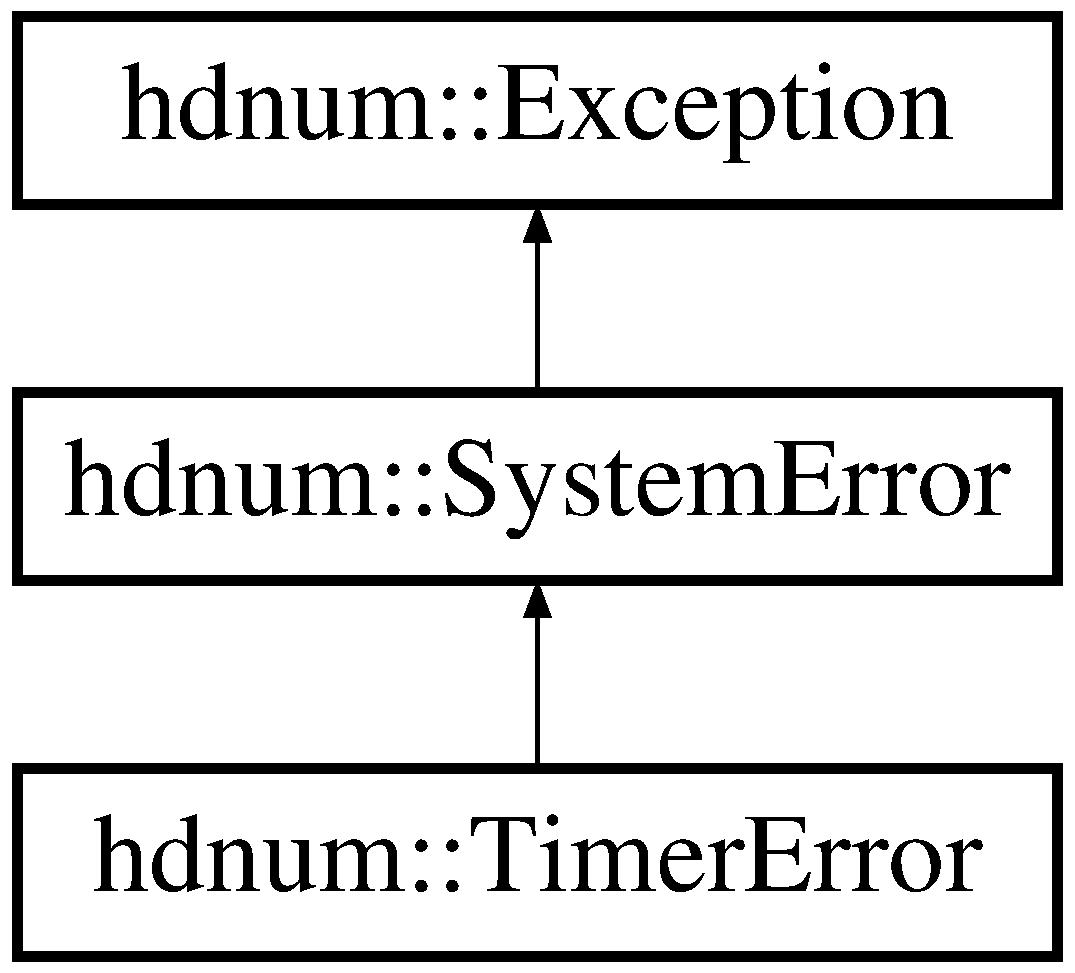
\includegraphics[height=3cm]{classhdnum_1_1TimerError}
\end{center}
\end{figure}


\subsection{Detailed Description}
Exception thrown by the \hyperlink{classhdnum_1_1Timer}{Timer} class 

The documentation for this class was generated from the following file:\begin{DoxyCompactItemize}
\item 
src/\hyperlink{timer_8hh}{timer.hh}\end{DoxyCompactItemize}

\hypertarget{classstd_1_1vector}{
\section{vector Class Reference}
\label{classstd_1_1vector}\index{std::vector@{std::vector}}
}


Inherited by \hyperlink{classhdnum_1_1Vector}{hdnum::Vector$<$ number\_\-type $>$}, and \hyperlink{classhdnum_1_1Vector}{hdnum::Vector$<$ size\_\-type $>$}.



The documentation for this class was generated from the following file:\begin{DoxyCompactItemize}
\item 
src/vector.hh\end{DoxyCompactItemize}

\hypertarget{classhdnum_1_1Vector}{
\section{hdnum::Vector$<$ REAL $>$ Class Template Reference}
\label{classhdnum_1_1Vector}\index{hdnum::Vector@{hdnum::Vector}}
}


Class with mathematical vector operations.  




{\ttfamily \#include $<$vector.hh$>$}

\subsection*{Public Types}
\begin{DoxyCompactItemize}
\item 
\hypertarget{classhdnum_1_1Vector_a21a951721fb2e12d8e1550f637fcb06d}{
typedef std::size\_\-t \hyperlink{classhdnum_1_1Vector_a21a951721fb2e12d8e1550f637fcb06d}{size\_\-type}}
\label{classhdnum_1_1Vector_a21a951721fb2e12d8e1550f637fcb06d}

\begin{DoxyCompactList}\small\item\em Type used for array indices. \item\end{DoxyCompactList}\end{DoxyCompactItemize}
\subsection*{Public Member Functions}
\begin{DoxyCompactItemize}
\item 
\hypertarget{classhdnum_1_1Vector_a25444a918837812c5cc7ad66e1aa77e2}{
{\bfseries Vector} (const size\_\-t size, const REAL defaultvalue\_\-=0)}
\label{classhdnum_1_1Vector_a25444a918837812c5cc7ad66e1aa77e2}

\item 
\hyperlink{classhdnum_1_1Vector}{Vector} \& \hyperlink{classhdnum_1_1Vector_a1cc1f492977e5e6dcf600024b2a75492}{operator=} (const REAL value)
\begin{DoxyCompactList}\small\item\em Assign all values of the \hyperlink{classhdnum_1_1Vector}{Vector} from one scalar value: x = value. \item\end{DoxyCompactList}\item 
\hyperlink{classhdnum_1_1Vector}{Vector} \& \hyperlink{classhdnum_1_1Vector_af410c46d0f56d02d15ff53aecb1b5701}{operator$\ast$=} (const REAL value)
\begin{DoxyCompactList}\small\item\em Assigning a vector from a given vector: x = y. \item\end{DoxyCompactList}\item 
\hypertarget{classhdnum_1_1Vector_ab5ac2b488ae212f37783fb601024c84f}{
\hyperlink{classhdnum_1_1Vector}{Vector} \& {\bfseries operator/=} (const REAL value)}
\label{classhdnum_1_1Vector_ab5ac2b488ae212f37783fb601024c84f}

\item 
\hypertarget{classhdnum_1_1Vector_a642332d4aa66727ae7bb5b6f36688278}{
\hyperlink{classhdnum_1_1Vector}{Vector} \& {\bfseries operator+=} (const \hyperlink{classhdnum_1_1Vector}{Vector} \&y)}
\label{classhdnum_1_1Vector_a642332d4aa66727ae7bb5b6f36688278}

\item 
\hypertarget{classhdnum_1_1Vector_ac6fecb3e3fe595dc19bf7571398608d0}{
\hyperlink{classhdnum_1_1Vector}{Vector} \& {\bfseries operator-\/=} (const \hyperlink{classhdnum_1_1Vector}{Vector} \&y)}
\label{classhdnum_1_1Vector_ac6fecb3e3fe595dc19bf7571398608d0}

\item 
\hypertarget{classhdnum_1_1Vector_a5b6de8d247ad4ed6b62cfcfd6264b958}{
\hyperlink{classhdnum_1_1Vector}{Vector} \& {\bfseries update} (const REAL alpha, const \hyperlink{classhdnum_1_1Vector}{Vector} \&y)}
\label{classhdnum_1_1Vector_a5b6de8d247ad4ed6b62cfcfd6264b958}

\item 
REAL \hyperlink{classhdnum_1_1Vector_aef63f9bb0fd5490d989317559ab5417e}{operator$\ast$} (\hyperlink{classhdnum_1_1Vector}{Vector} \&x) const 
\begin{DoxyCompactList}\small\item\em Inner product with another vector. \item\end{DoxyCompactList}\item 
\hyperlink{classhdnum_1_1Vector}{Vector} \hyperlink{classhdnum_1_1Vector_a15b3fcda96f788a4de617d24f6974647}{operator+} (\hyperlink{classhdnum_1_1Vector}{Vector} \&x) const 
\begin{DoxyCompactList}\small\item\em Adding two vectors x+y. \item\end{DoxyCompactList}\item 
\hyperlink{classhdnum_1_1Vector}{Vector} \hyperlink{classhdnum_1_1Vector_af44713378f5150c2d12a981e6641f09a}{operator-\/} (\hyperlink{classhdnum_1_1Vector}{Vector} \&x) const 
\begin{DoxyCompactList}\small\item\em vector subtraction x-\/y \item\end{DoxyCompactList}\item 
\hypertarget{classhdnum_1_1Vector_a861d14f56f15f030baa8e77a6fd7294d}{
REAL \hyperlink{classhdnum_1_1Vector_a861d14f56f15f030baa8e77a6fd7294d}{two\_\-norm\_\-2} () const }
\label{classhdnum_1_1Vector_a861d14f56f15f030baa8e77a6fd7294d}

\begin{DoxyCompactList}\small\item\em Square of the Euclidean norm. \item\end{DoxyCompactList}\item 
REAL \hyperlink{classhdnum_1_1Vector_a5d44d50fe956733a43a59300c559c13c}{two\_\-norm} () const 
\begin{DoxyCompactList}\small\item\em Euclidean norm of a vector. \item\end{DoxyCompactList}\item 
\hypertarget{classhdnum_1_1Vector_ae95ec8cc3365696d65b4c7a51c61522d}{
bool \hyperlink{classhdnum_1_1Vector_ae95ec8cc3365696d65b4c7a51c61522d}{scientific} () const }
\label{classhdnum_1_1Vector_ae95ec8cc3365696d65b4c7a51c61522d}

\begin{DoxyCompactList}\small\item\em pretty-\/print output property: true = scientific, false = fixed point representation \item\end{DoxyCompactList}\item 
void \hyperlink{classhdnum_1_1Vector_ab9befaae588c670c4bc2a848d9072b97}{scientific} (bool b) const 
\begin{DoxyCompactList}\small\item\em scientific(true) is the default, scientific(false) switches to the fixed point representation \item\end{DoxyCompactList}\item 
\hypertarget{classhdnum_1_1Vector_a232022d5d9ff38b63c1495823875cec2}{
std::size\_\-t {\bfseries width} () const }
\label{classhdnum_1_1Vector_a232022d5d9ff38b63c1495823875cec2}

\item 
\hypertarget{classhdnum_1_1Vector_a78d2ee2c0096fbe9cbe5f8d1784e568c}{
void {\bfseries width} (std::size\_\-t i) const }
\label{classhdnum_1_1Vector_a78d2ee2c0096fbe9cbe5f8d1784e568c}

\item 
\hypertarget{classhdnum_1_1Vector_abf554eaf0a7ecc0bad0417283592f0a9}{
std::size\_\-t {\bfseries iwidth} () const }
\label{classhdnum_1_1Vector_abf554eaf0a7ecc0bad0417283592f0a9}

\item 
\hypertarget{classhdnum_1_1Vector_a27b91a95ee7395f755e67ea75536c379}{
void {\bfseries iwidth} (std::size\_\-t i) const }
\label{classhdnum_1_1Vector_a27b91a95ee7395f755e67ea75536c379}

\item 
\hypertarget{classhdnum_1_1Vector_a0c3b0743b35e145ef9943f919410f072}{
std::size\_\-t {\bfseries precision} () const }
\label{classhdnum_1_1Vector_a0c3b0743b35e145ef9943f919410f072}

\item 
\hypertarget{classhdnum_1_1Vector_a721b7c7def445694f44ee1fe6e25ca90}{
void {\bfseries precision} (std::size\_\-t i) const }
\label{classhdnum_1_1Vector_a721b7c7def445694f44ee1fe6e25ca90}

\end{DoxyCompactItemize}
\subsection*{Related Functions}
(Note that these are not member functions.) \begin{DoxyCompactItemize}
\item 
{\footnotesize template$<$typename REAL $>$ }\\std::ostream \& \hyperlink{classhdnum_1_1Vector_a50345eaaa46f20d031cc751aa35e4232}{operator$<$$<$} (std::ostream \&os, const \hyperlink{classhdnum_1_1Vector}{Vector}$<$ REAL $>$ \&x)
\begin{DoxyCompactList}\small\item\em Output operator for \hyperlink{classhdnum_1_1Vector}{Vector}. \item\end{DoxyCompactList}\item 
{\footnotesize template$<$typename REAL $>$ }\\void \hyperlink{classhdnum_1_1Vector_aa4e036b4657b6e29d60f6f6c6638f403}{gnuplot} (const std::string \&fname, const \hyperlink{classhdnum_1_1Vector}{Vector}$<$ REAL $>$ x)
\begin{DoxyCompactList}\small\item\em Output contents of a \hyperlink{classhdnum_1_1Vector}{Vector} x to a text file named fname. \item\end{DoxyCompactList}\item 
{\footnotesize template$<$typename REAL $>$ }\\void \hyperlink{classhdnum_1_1Vector_a4e37b684a0a8fec1d254c6dc142d34dd}{readVectorFromFile} (const std::string \&filename, \hyperlink{classhdnum_1_1Vector}{Vector}$<$ REAL $>$ \&\hyperlink{classstd_1_1vector}{vector})
\begin{DoxyCompactList}\small\item\em Read vector from a text file. \item\end{DoxyCompactList}\item 
{\footnotesize template$<$class REAL $>$ }\\void \hyperlink{classhdnum_1_1Vector_acc994daebde7d1e9699353a5672d5a92}{fill} (\hyperlink{classhdnum_1_1Vector}{Vector}$<$ REAL $>$ \&x, const REAL \&t, const REAL \&dt)
\begin{DoxyCompactList}\small\item\em Fill vector, with entries starting at t, consecutively shifted by dt. \item\end{DoxyCompactList}\item 
{\footnotesize template$<$class REAL $>$ }\\void \hyperlink{classhdnum_1_1Vector_a99ec4439cc5942afee540708022372e7}{unitvector} (\hyperlink{classhdnum_1_1Vector}{Vector}$<$ REAL $>$ \&x, std::size\_\-t j)
\begin{DoxyCompactList}\small\item\em Defines j-\/th unitvector (j=0,...,n-\/1) where n = length of the vector. \item\end{DoxyCompactList}\end{DoxyCompactItemize}


\subsection{Detailed Description}
\subsubsection*{template$<$typename REAL$>$ class hdnum::Vector$<$ REAL $>$}

Class with mathematical vector operations. 

\subsection{Member Function Documentation}
\hypertarget{classhdnum_1_1Vector_aef63f9bb0fd5490d989317559ab5417e}{
\index{hdnum::Vector@{hdnum::Vector}!operator$\ast$@{operator$\ast$}}
\index{operator$\ast$@{operator$\ast$}!hdnum::Vector@{hdnum::Vector}}
\subsubsection[{operator$\ast$}]{\setlength{\rightskip}{0pt plus 5cm}template$<$typename REAL$>$ REAL {\bf hdnum::Vector}$<$ REAL $>$::operator$\ast$ ({\bf Vector}$<$ REAL $>$ \& {\em x}) const\hspace{0.3cm}{\ttfamily  \mbox{[}inline\mbox{]}}}}
\label{classhdnum_1_1Vector_aef63f9bb0fd5490d989317559ab5417e}


Inner product with another vector. 

{\bfseries Example:} 
\begin{DoxyCode}
hdnum::Vector<double> x(2);
x.scientific(false); // set fixed point display mode
x[0] = 12.0;
x[1] = 3.0;
std::cout << "x=" << x << std::endl;
hdnum::Vector<double> y(2);
y[0] = 4.0;
y[1] = -1.0;
std::cout << "y=" << y << std::endl;
double s = x*y;
std::cout << "s = x*y = " << s << std::endl;
\end{DoxyCode}


{\bfseries Output:} \begin{DoxyVerb}
x=
[ 0]     12.0000000
[ 1]      3.0000000

y=
[ 0]      4.0000000
[ 1]     -1.0000000

s = x*y = 45.0000000
	  \end{DoxyVerb}
 \hypertarget{classhdnum_1_1Vector_af410c46d0f56d02d15ff53aecb1b5701}{
\index{hdnum::Vector@{hdnum::Vector}!operator$\ast$=@{operator$\ast$=}}
\index{operator$\ast$=@{operator$\ast$=}!hdnum::Vector@{hdnum::Vector}}
\subsubsection[{operator$\ast$=}]{\setlength{\rightskip}{0pt plus 5cm}template$<$typename REAL$>$ {\bf Vector}\& {\bf hdnum::Vector}$<$ REAL $>$::operator$\ast$= (const REAL {\em value})\hspace{0.3cm}{\ttfamily  \mbox{[}inline\mbox{]}}}}
\label{classhdnum_1_1Vector_af410c46d0f56d02d15ff53aecb1b5701}


Assigning a vector from a given vector: x = y. 

{\bfseries Example:} 
\begin{DoxyCode}
hdnum::Vector<double> x(4);
hdnum::Vector<double> y(4);
x[0] = 1.23;
x[1] = 2.31;
x[2] = 4.54;
x[3] = 9.98;
std::cout << "x=" << x << std::endl;
y = x;
std::cout << "y=" << y << std::endl;
\end{DoxyCode}


{\bfseries Output:} \begin{DoxyVerb}
x=
[ 0]  1.2300000e+00
[ 1]  2.3100000e+00
[ 2]  4.5400000e+00
[ 3]  9.9800000e+00

y=
[ 0]  1.2300000e+00
[ 1]  2.3100000e+00
[ 2]  4.5400000e+00
[ 3]  9.9800000e+00
	  \end{DoxyVerb}
 \hypertarget{classhdnum_1_1Vector_a15b3fcda96f788a4de617d24f6974647}{
\index{hdnum::Vector@{hdnum::Vector}!operator+@{operator+}}
\index{operator+@{operator+}!hdnum::Vector@{hdnum::Vector}}
\subsubsection[{operator+}]{\setlength{\rightskip}{0pt plus 5cm}template$<$typename REAL$>$ {\bf Vector} {\bf hdnum::Vector}$<$ REAL $>$::operator+ ({\bf Vector}$<$ REAL $>$ \& {\em x}) const\hspace{0.3cm}{\ttfamily  \mbox{[}inline\mbox{]}}}}
\label{classhdnum_1_1Vector_a15b3fcda96f788a4de617d24f6974647}


Adding two vectors x+y. 

{\bfseries Example:} 
\begin{DoxyCode}
hdnum::Vector<double> x(2);
x.scientific(false); // set fixed point display mode
x[0] = 12.0;
x[1] = 3.0;
std::cout << "x=" << x << std::endl;
hdnum::Vector<double> y(2);
y[0] = 4.0;
y[1] = -1.0;
std::cout << "y=" << y << std::endl;
std::cout << "x+y = " << x+y << std::endl;
\end{DoxyCode}


{\bfseries Output:} \begin{DoxyVerb}
x=
[ 0]     12.0000000
[ 1]      3.0000000

y=
[ 0]      4.0000000
[ 1]     -1.0000000

x+y = 
[ 0]     16.0000000
[ 1]      2.0000000
	  \end{DoxyVerb}
 \hypertarget{classhdnum_1_1Vector_af44713378f5150c2d12a981e6641f09a}{
\index{hdnum::Vector@{hdnum::Vector}!operator-\/@{operator-\/}}
\index{operator-\/@{operator-\/}!hdnum::Vector@{hdnum::Vector}}
\subsubsection[{operator-\/}]{\setlength{\rightskip}{0pt plus 5cm}template$<$typename REAL$>$ {\bf Vector} {\bf hdnum::Vector}$<$ REAL $>$::operator-\/ ({\bf Vector}$<$ REAL $>$ \& {\em x}) const\hspace{0.3cm}{\ttfamily  \mbox{[}inline\mbox{]}}}}
\label{classhdnum_1_1Vector_af44713378f5150c2d12a981e6641f09a}


vector subtraction x-\/y 

{\bfseries Example:} 
\begin{DoxyCode}
hdnum::Vector<double> x(2);
x.scientific(false); // set fixed point display mode
x[0] = 12.0;
x[1] = 3.0;
std::cout << "x=" << x << std::endl;
hdnum::Vector<double> y(2);
y[0] = 4.0;
y[1] = -1.0;
std::cout << "y=" << y << std::endl;
std::cout << "x-y = " << x-y << std::endl;
\end{DoxyCode}


{\bfseries Output:} \begin{DoxyVerb}
x=
[ 0]     12.0000000
[ 1]      3.0000000

y=
[ 0]      4.0000000
[ 1]     -1.0000000

x-y = 
[ 0]      8.0000000
[ 1]      4.0000000
	  \end{DoxyVerb}
 \hypertarget{classhdnum_1_1Vector_a1cc1f492977e5e6dcf600024b2a75492}{
\index{hdnum::Vector@{hdnum::Vector}!operator=@{operator=}}
\index{operator=@{operator=}!hdnum::Vector@{hdnum::Vector}}
\subsubsection[{operator=}]{\setlength{\rightskip}{0pt plus 5cm}template$<$typename REAL$>$ {\bf Vector}\& {\bf hdnum::Vector}$<$ REAL $>$::operator= (const REAL {\em value})\hspace{0.3cm}{\ttfamily  \mbox{[}inline\mbox{]}}}}
\label{classhdnum_1_1Vector_a1cc1f492977e5e6dcf600024b2a75492}


Assign all values of the \hyperlink{classhdnum_1_1Vector}{Vector} from one scalar value: x = value. 

{\bfseries Example:} 
\begin{DoxyCode}
hdnum::Vector<double> x(4);
x = 1.23;
std::cout << "x=" << x << std::endl;
\end{DoxyCode}


{\bfseries Output:} \begin{DoxyVerb}
x=
[ 0]  1.2340000e+00
[ 1]  1.2340000e+00
[ 2]  1.2340000e+00
[ 3]  1.2340000e+00
	  \end{DoxyVerb}
 \hypertarget{classhdnum_1_1Vector_ab9befaae588c670c4bc2a848d9072b97}{
\index{hdnum::Vector@{hdnum::Vector}!scientific@{scientific}}
\index{scientific@{scientific}!hdnum::Vector@{hdnum::Vector}}
\subsubsection[{scientific}]{\setlength{\rightskip}{0pt plus 5cm}template$<$typename REAL$>$ void {\bf hdnum::Vector}$<$ REAL $>$::scientific (bool {\em b}) const\hspace{0.3cm}{\ttfamily  \mbox{[}inline\mbox{]}}}}
\label{classhdnum_1_1Vector_ab9befaae588c670c4bc2a848d9072b97}


scientific(true) is the default, scientific(false) switches to the fixed point representation 

{\bfseries Example:} 
\begin{DoxyCode}
  hdnum::Vector<double> x(3);
  x[0] = 2.0;
  x[1] = 2.0;
  x[2] = 1.0;
  std::cout << "x=" << x << std::endl;
  x.scientific(false); // set fixed point display mode
  std::cout << "x=" << x << std::endl;
\end{DoxyCode}


{\bfseries Output:} \begin{DoxyVerb}
x=
[ 0]  2.0000000e+00
[ 1]  2.0000000e+00
[ 2]  1.0000000e+00

x=
[ 0]      2.0000000
[ 1]      2.0000000
[ 2]      1.0000000
	  \end{DoxyVerb}
 \hypertarget{classhdnum_1_1Vector_a5d44d50fe956733a43a59300c559c13c}{
\index{hdnum::Vector@{hdnum::Vector}!two\_\-norm@{two\_\-norm}}
\index{two\_\-norm@{two\_\-norm}!hdnum::Vector@{hdnum::Vector}}
\subsubsection[{two\_\-norm}]{\setlength{\rightskip}{0pt plus 5cm}template$<$typename REAL$>$ REAL {\bf hdnum::Vector}$<$ REAL $>$::two\_\-norm () const\hspace{0.3cm}{\ttfamily  \mbox{[}inline\mbox{]}}}}
\label{classhdnum_1_1Vector_a5d44d50fe956733a43a59300c559c13c}


Euclidean norm of a vector. 

{\bfseries Example:} 
\begin{DoxyCode}
  hdnum::Vector<double> x(3);
  x.scientific(false); // set fixed point display mode
  x[0] = 2.0;
  x[1] = 2.0;
  x[2] = 1.0;
  std::cout << "x=" << x << std::endl;
  std::cout << "euclidean norm of x = " << x.two_norm() << std::endl;
\end{DoxyCode}


{\bfseries Output:} \begin{DoxyVerb}
x=
[ 0]      2.0000000
[ 1]      2.0000000
[ 2]      1.0000000

euclidean norm of x = 3.0000000
	  \end{DoxyVerb}
 

\subsection{Friends And Related Function Documentation}
\hypertarget{classhdnum_1_1Vector_acc994daebde7d1e9699353a5672d5a92}{
\index{hdnum::Vector@{hdnum::Vector}!fill@{fill}}
\index{fill@{fill}!hdnum::Vector@{hdnum::Vector}}
\subsubsection[{fill}]{\setlength{\rightskip}{0pt plus 5cm}template$<$class REAL $>$ void fill ({\bf Vector}$<$ REAL $>$ \& {\em x}, \/  const REAL \& {\em t}, \/  const REAL \& {\em dt})\hspace{0.3cm}{\ttfamily  \mbox{[}related\mbox{]}}}}
\label{classhdnum_1_1Vector_acc994daebde7d1e9699353a5672d5a92}


Fill vector, with entries starting at t, consecutively shifted by dt. 

{\bfseries Example:} 
\begin{DoxyCode}
  hdnum::Vector<double> x(5);
  fill(x,2.01,0.1);
  x.scientific(false); // set fixed point display mode
  std::cout << "x=" << x << std::endl;
\end{DoxyCode}


{\bfseries Output:} \begin{DoxyVerb}
x=
[ 0]      2.0100000
[ 1]      2.1100000
[ 2]      2.2100000
[ 3]      2.3100000
[ 4]      2.4100000
	  \end{DoxyVerb}
 \hypertarget{classhdnum_1_1Vector_aa4e036b4657b6e29d60f6f6c6638f403}{
\index{hdnum::Vector@{hdnum::Vector}!gnuplot@{gnuplot}}
\index{gnuplot@{gnuplot}!hdnum::Vector@{hdnum::Vector}}
\subsubsection[{gnuplot}]{\setlength{\rightskip}{0pt plus 5cm}template$<$typename REAL $>$ void gnuplot (const std::string \& {\em fname}, \/  const {\bf Vector}$<$ REAL $>$ {\em x})\hspace{0.3cm}{\ttfamily  \mbox{[}related\mbox{]}}}}
\label{classhdnum_1_1Vector_aa4e036b4657b6e29d60f6f6c6638f403}


Output contents of a \hyperlink{classhdnum_1_1Vector}{Vector} x to a text file named fname. 

{\bfseries Example:} 
\begin{DoxyCode}
  hdnum::Vector<double> x(5);
  unitvector(x,3);
  x.scientific(false); // set fixed point display mode
  gnuplot("test.dat",x);
\end{DoxyCode}


{\bfseries Output:} \begin{DoxyVerb}
Contents of 'test.dat':
              0      0.0000000
              1      0.0000000
              2      0.0000000
              3      1.0000000
              4      0.0000000
	  \end{DoxyVerb}
 \hypertarget{classhdnum_1_1Vector_a50345eaaa46f20d031cc751aa35e4232}{
\index{hdnum::Vector@{hdnum::Vector}!operator$<$$<$@{operator$<$$<$}}
\index{operator$<$$<$@{operator$<$$<$}!hdnum::Vector@{hdnum::Vector}}
\subsubsection[{operator$<$$<$}]{\setlength{\rightskip}{0pt plus 5cm}template$<$typename REAL $>$ std::ostream \& operator$<$$<$ (std::ostream \& {\em os}, \/  const {\bf Vector}$<$ REAL $>$ \& {\em x})\hspace{0.3cm}{\ttfamily  \mbox{[}related\mbox{]}}}}
\label{classhdnum_1_1Vector_a50345eaaa46f20d031cc751aa35e4232}


Output operator for \hyperlink{classhdnum_1_1Vector}{Vector}. 

{\bfseries Example:} 
\begin{DoxyCode}
  hdnum::Vector<double> x(3);
  x[0] = 2.0;
  x[1] = 2.0;
  x[2] = 1.0;
  std::cout << "x=" << x << std::endl;
\end{DoxyCode}


{\bfseries Output:} \begin{DoxyVerb}
x=
[ 0]  2.0000000e+00
[ 1]  2.0000000e+00
[ 2]  1.0000000e+00
	  \end{DoxyVerb}
 \hypertarget{classhdnum_1_1Vector_a4e37b684a0a8fec1d254c6dc142d34dd}{
\index{hdnum::Vector@{hdnum::Vector}!readVectorFromFile@{readVectorFromFile}}
\index{readVectorFromFile@{readVectorFromFile}!hdnum::Vector@{hdnum::Vector}}
\subsubsection[{readVectorFromFile}]{\setlength{\rightskip}{0pt plus 5cm}template$<$typename REAL $>$ void readVectorFromFile (const std::string \& {\em filename}, \/  {\bf Vector}$<$ REAL $>$ \& {\em vector})\hspace{0.3cm}{\ttfamily  \mbox{[}related\mbox{]}}}}
\label{classhdnum_1_1Vector_a4e37b684a0a8fec1d254c6dc142d34dd}


Read vector from a text file. 


\begin{DoxyParams}{Parameters}
\item[\mbox{$\leftarrow$} {\em filename}]name of the text file \item[\mbox{$\leftrightarrow$} {\em x}]reference to a \hyperlink{classhdnum_1_1Vector}{Vector}\end{DoxyParams}
{\bfseries Example:} 
\begin{DoxyCode}
  hdnum::Vector<number> x;
  readVectorFromFile("x.dat", x );
  std::cout << "x=" << x << std::endl;
\end{DoxyCode}


{\bfseries Output:} \begin{DoxyVerb}
Contents of "x.dat":
1.0
2.0
3.0

would give:
x=
[ 0]  1.0000000e+00
[ 1]  2.0000000e+00
[ 2]  3.0000000e+00
	\end{DoxyVerb}
 \hypertarget{classhdnum_1_1Vector_a99ec4439cc5942afee540708022372e7}{
\index{hdnum::Vector@{hdnum::Vector}!unitvector@{unitvector}}
\index{unitvector@{unitvector}!hdnum::Vector@{hdnum::Vector}}
\subsubsection[{unitvector}]{\setlength{\rightskip}{0pt plus 5cm}template$<$class REAL $>$ void unitvector ({\bf Vector}$<$ REAL $>$ \& {\em x}, \/  std::size\_\-t {\em j})\hspace{0.3cm}{\ttfamily  \mbox{[}related\mbox{]}}}}
\label{classhdnum_1_1Vector_a99ec4439cc5942afee540708022372e7}


Defines j-\/th unitvector (j=0,...,n-\/1) where n = length of the vector. 

{\bfseries Example:} 
\begin{DoxyCode}
  hdnum::Vector<double> x(5);
  unitvector(x,3);
  x.scientific(false); // set fixed point display mode
  std::cout << "x=" << x << std::endl;
\end{DoxyCode}


{\bfseries Output:} \begin{DoxyVerb}
x=
[ 0]      0.0000000
[ 1]      0.0000000
[ 2]      0.0000000
[ 3]      1.0000000
[ 4]      0.0000000
	  \end{DoxyVerb}
 

The documentation for this class was generated from the following file:\begin{DoxyCompactItemize}
\item 
src/vector.hh\end{DoxyCompactItemize}

\chapter{File Documentation}
\hypertarget{array_8hh}{
\section{src/array.hh File Reference}
\label{array_8hh}\index{src/array.hh@{src/array.hh}}
}


This file implements a basic dynamic array class.  


\subsection*{Classes}
\begin{DoxyCompactItemize}
\item 
class \hyperlink{classhdnum_1_1Array}{hdnum::Array$<$ T $>$}
\begin{DoxyCompactList}\small\item\em A basic dynamic array class. \item\end{DoxyCompactList}\end{DoxyCompactItemize}


\subsection{Detailed Description}
This file implements a basic dynamic array class. 
\hypertarget{countablearray_8hh}{
\section{src/countablearray.hh File Reference}
\label{countablearray_8hh}\index{src/countablearray.hh@{src/countablearray.hh}}
}


This file implements a basic dynamic array class.  


{\ttfamily \#include \char`\"{}countingptr.hh\char`\"{}}\par
{\ttfamily \#include $<$iostream$>$}\par
\subsection*{Classes}
\begin{DoxyCompactItemize}
\item 
class \hyperlink{classhdnum_1_1CountableArray}{hdnum::CountableArray$<$ T $>$}
\begin{DoxyCompactList}\small\item\em Dynamic array that can be used with the reference counting pointer. \item\end{DoxyCompactList}\end{DoxyCompactItemize}


\subsection{Detailed Description}
This file implements a basic dynamic array class. 
\hypertarget{countingptr_8hh}{
\section{src/countingptr.hh File Reference}
\label{countingptr_8hh}\index{src/countingptr.hh@{src/countingptr.hh}}
}


This file implements a counting pointer with configurable memory management policy Adapted from dune-\/pdelab.  


{\ttfamily \#include $<$iostream$>$}\par
\subsection*{Classes}
\begin{DoxyCompactItemize}
\item 
class \hyperlink{classhdnum_1_1NondeletingMemoryManagementPolicy}{hdnum::NondeletingMemoryManagementPolicy}
\begin{DoxyCompactList}\small\item\em Don't delete target if reference count reaches zero. \item\end{DoxyCompactList}\item 
class \hyperlink{classhdnum_1_1DeletingMemoryManagementPolicy}{hdnum::DeletingMemoryManagementPolicy}
\begin{DoxyCompactList}\small\item\em Delete target if reference count reaches zero. \item\end{DoxyCompactList}\item 
class \hyperlink{classhdnum_1_1CP}{hdnum::CP$<$ T, P $>$}
\begin{DoxyCompactList}\small\item\em Pointer with a reference count in the pointed-\/to object. \item\end{DoxyCompactList}\item 
class \hyperlink{classhdnum_1_1CountableException}{hdnum::CountableException}
\item 
class \hyperlink{classhdnum_1_1Countable}{hdnum::Countable}
\begin{DoxyCompactList}\small\item\em Base class for object pointed to by \hyperlink{classhdnum_1_1CP}{CP}. \item\end{DoxyCompactList}\end{DoxyCompactItemize}


\subsection{Detailed Description}
This file implements a counting pointer with configurable memory management policy Adapted from dune-\/pdelab. 
\hypertarget{exceptions_8hh}{
\section{src/exceptions.hh File Reference}
\label{exceptions_8hh}\index{src/exceptions.hh@{src/exceptions.hh}}
}


A few common exception classes.  


{\ttfamily \#include $<$string$>$}\par
{\ttfamily \#include $<$sstream$>$}\par
\subsection*{Classes}
\begin{DoxyCompactItemize}
\item 
class \hyperlink{classhdnum_1_1Exception}{hdnum::Exception}
\begin{DoxyCompactList}\small\item\em Base class for Exceptions. \item\end{DoxyCompactList}\item 
class \hyperlink{classhdnum_1_1IOError}{hdnum::IOError}
\begin{DoxyCompactList}\small\item\em Default exception class for I/O errors. \item\end{DoxyCompactList}\item 
class \hyperlink{classhdnum_1_1MathError}{hdnum::MathError}
\begin{DoxyCompactList}\small\item\em Default exception class for mathematical errors. \item\end{DoxyCompactList}\item 
class \hyperlink{classhdnum_1_1RangeError}{hdnum::RangeError}
\begin{DoxyCompactList}\small\item\em Default exception class for range errors. \item\end{DoxyCompactList}\item 
class \hyperlink{classhdnum_1_1NotImplemented}{hdnum::NotImplemented}
\begin{DoxyCompactList}\small\item\em Default exception for dummy implementations. \item\end{DoxyCompactList}\item 
class \hyperlink{classhdnum_1_1SystemError}{hdnum::SystemError}
\begin{DoxyCompactList}\small\item\em Default exception class for OS errors. \item\end{DoxyCompactList}\item 
class \hyperlink{classhdnum_1_1OutOfMemoryError}{hdnum::OutOfMemoryError}
\begin{DoxyCompactList}\small\item\em Default exception if memory allocation fails. \item\end{DoxyCompactList}\item 
class \hyperlink{classhdnum_1_1InvalidStateException}{hdnum::InvalidStateException}
\begin{DoxyCompactList}\small\item\em Default exception if a function was called while the object is not in a valid state for that function. \item\end{DoxyCompactList}\item 
class \hyperlink{classhdnum_1_1ErrorException}{hdnum::ErrorException}
\begin{DoxyCompactList}\small\item\em General Error. \item\end{DoxyCompactList}\end{DoxyCompactItemize}
\subsection*{Defines}
\begin{DoxyCompactItemize}
\item 
\hypertarget{exceptions_8hh_a3166b62636d7a133db5150ce192d0ad3}{
\#define {\bfseries THROWSPEC}(E)~\#E $<$$<$ \char`\"{}: \char`\"{}}
\label{exceptions_8hh_a3166b62636d7a133db5150ce192d0ad3}

\item 
\#define \hyperlink{exceptions_8hh_a7385bc4ca18aaff3f509a30bde2567c0}{HDNUM\_\-THROW}(E, m)
\item 
\#define {\bfseries HDNUM\_\-ERROR}(m)
\end{DoxyCompactItemize}
\subsection*{Functions}
\begin{DoxyCompactItemize}
\item 
\hypertarget{namespacehdnum_a892de125bed4e6f2dcc4a55300573e32}{
std::ostream \& {\bfseries hdnum::operator$<$$<$} (std::ostream \&stream, const Exception \&e)}
\label{namespacehdnum_a892de125bed4e6f2dcc4a55300573e32}

\end{DoxyCompactItemize}


\subsection{Detailed Description}
A few common exception classes. This file defines a common framework for generating exception subclasses and to throw them in a simple manner. Taken from the DUNE project www.dune-\/project.org 

\subsection{Define Documentation}
\hypertarget{exceptions_8hh_ac5258d45eb46dc2d92f02f0c61bd58f9}{
\index{exceptions.hh@{exceptions.hh}!HDNUM\_\-ERROR@{HDNUM\_\-ERROR}}
\index{HDNUM\_\-ERROR@{HDNUM\_\-ERROR}!exceptions.hh@{exceptions.hh}}
\subsubsection[{HDNUM\_\-ERROR}]{\setlength{\rightskip}{0pt plus 5cm}\#define HDNUM\_\-ERROR(m)}}
\label{exceptions_8hh_ac5258d45eb46dc2d92f02f0c61bd58f9}
{\bfseries Value:}
\begin{DoxyCode}
do { hdnum::ErrorException th__ex; std::ostringstream th__out;          \
        th__out << THROWSPEC(hdnum::ErrorException) << m; \
        th__ex.message(th__out.str()); \
        std::cout << th__ex.what() << std::endl; \
        throw th__ex;                              \
  } while (0)
\end{DoxyCode}
\hypertarget{exceptions_8hh_a7385bc4ca18aaff3f509a30bde2567c0}{
\index{exceptions.hh@{exceptions.hh}!HDNUM\_\-THROW@{HDNUM\_\-THROW}}
\index{HDNUM\_\-THROW@{HDNUM\_\-THROW}!exceptions.hh@{exceptions.hh}}
\subsubsection[{HDNUM\_\-THROW}]{\setlength{\rightskip}{0pt plus 5cm}\#define HDNUM\_\-THROW(E, \/  m)}}
\label{exceptions_8hh_a7385bc4ca18aaff3f509a30bde2567c0}
{\bfseries Value:}
\begin{DoxyCode}
do { E th__ex; std::ostringstream th__out;              \
        th__out << THROWSPEC(E) << m; th__ex.message(th__out.str()); throw th__ex
      ; \
  } while (0)
\end{DoxyCode}
Macro to throw an exception


\begin{DoxyParams}{Parameters}
\item[{\em E}]exception class derived from Dune::Exception \item[{\em m}]reason for this exception in ostream-\/notation\end{DoxyParams}
Example:


\begin{DoxyCode}
        if (filehandle == 0)
    DUNE_THROW(FileError, "Could not open " << filename << " for reading!")
\end{DoxyCode}


DUNE\_\-THROW automatically adds information about the exception thrown to the text. If DUNE\_\-DEVEL\_\-MODE is defined more detail about the function where the exception happened is included. This mode can be activated via the {\ttfamily -\/-\/enable-\/dunedevel} switch of {\ttfamily }./configure 
\hypertarget{lr_8hh}{
\section{src/lr.hh File Reference}
\label{lr_8hh}\index{src/lr.hh@{src/lr.hh}}
}


This file implements a generic and dynamic vector class.  


{\ttfamily \#include \char`\"{}vector.hh\char`\"{}}\par
{\ttfamily \#include \char`\"{}matrix.hh\char`\"{}}\par
{\ttfamily \#include $<$iostream$>$}\par
{\ttfamily \#include $<$iomanip$>$}\par
{\ttfamily \#include $<$string$>$}\par
{\ttfamily \#include $<$fstream$>$}\par
{\ttfamily \#include \char`\"{}countingptr.hh\char`\"{}}\par
{\ttfamily \#include \char`\"{}array.hh\char`\"{}}\par
{\ttfamily \#include $<$sstream$>$}\par
\subsection*{Functions}
\begin{DoxyCompactItemize}
\item 
\hypertarget{namespacehdnum_aa6579c01f220999e670f956774bd85c7}{
{\footnotesize template$<$class T $>$ }\\void \hyperlink{namespacehdnum_aa6579c01f220999e670f956774bd85c7}{hdnum::lr} (Matrix$<$ T $>$ \&A, Array$<$ std::size\_\-t $>$ \&p)}
\label{namespacehdnum_aa6579c01f220999e670f956774bd85c7}

\begin{DoxyCompactList}\small\item\em compute lr decomposition of A with first nonzero pivoting \item\end{DoxyCompactList}\item 
\hypertarget{namespacehdnum_a9ab161adff3c1341fcf1cffb6b503a3a}{
{\footnotesize template$<$class T $>$ }\\T \hyperlink{namespacehdnum_a9ab161adff3c1341fcf1cffb6b503a3a}{hdnum::abs} (const T \&t)}
\label{namespacehdnum_a9ab161adff3c1341fcf1cffb6b503a3a}

\begin{DoxyCompactList}\small\item\em our own abs class that works also for multiprecision types \item\end{DoxyCompactList}\item 
\hypertarget{namespacehdnum_a1ddad586daab7c3757cb7049a9330f30}{
{\footnotesize template$<$class T $>$ }\\void \hyperlink{namespacehdnum_a1ddad586daab7c3757cb7049a9330f30}{hdnum::lr\_\-partialpivot} (Matrix$<$ T $>$ \&A, Array$<$ std::size\_\-t $>$ \&p)}
\label{namespacehdnum_a1ddad586daab7c3757cb7049a9330f30}

\begin{DoxyCompactList}\small\item\em lr decomposition of A with column pivoting \item\end{DoxyCompactList}\item 
\hypertarget{namespacehdnum_a18307e1ea7ffb87dff8628ccbf723545}{
{\footnotesize template$<$class T $>$ }\\void \hyperlink{namespacehdnum_a18307e1ea7ffb87dff8628ccbf723545}{hdnum::lr\_\-fullpivot} (Matrix$<$ T $>$ \&A, Array$<$ std::size\_\-t $>$ \&p, Array$<$ std::size\_\-t $>$ \&q)}
\label{namespacehdnum_a18307e1ea7ffb87dff8628ccbf723545}

\begin{DoxyCompactList}\small\item\em lr decomposition of A with full pivoting \item\end{DoxyCompactList}\item 
\hypertarget{namespacehdnum_afebc7f6525181712ff86cf82b21200e3}{
{\footnotesize template$<$class T $>$ }\\void \hyperlink{namespacehdnum_afebc7f6525181712ff86cf82b21200e3}{hdnum::permute\_\-forward} (const Array$<$ std::size\_\-t $>$ \&p, Vector$<$ T $>$ \&b)}
\label{namespacehdnum_afebc7f6525181712ff86cf82b21200e3}

\begin{DoxyCompactList}\small\item\em apply permutations to a right hand side vector \item\end{DoxyCompactList}\item 
\hypertarget{namespacehdnum_ad7a4d91e943ea48de3d44d83649b118a}{
{\footnotesize template$<$class T $>$ }\\void \hyperlink{namespacehdnum_ad7a4d91e943ea48de3d44d83649b118a}{hdnum::permute\_\-backward} (const Array$<$ std::size\_\-t $>$ \&q, Vector$<$ T $>$ \&z)}
\label{namespacehdnum_ad7a4d91e943ea48de3d44d83649b118a}

\begin{DoxyCompactList}\small\item\em apply permutations to a solution vector \item\end{DoxyCompactList}\item 
\hypertarget{namespacehdnum_a8c1b2c65058180de1615d4c1ed0d2477}{
{\footnotesize template$<$class T $>$ }\\void \hyperlink{namespacehdnum_a8c1b2c65058180de1615d4c1ed0d2477}{hdnum::row\_\-equilibrate} (Matrix$<$ T $>$ \&A, Vector$<$ T $>$ \&s)}
\label{namespacehdnum_a8c1b2c65058180de1615d4c1ed0d2477}

\begin{DoxyCompactList}\small\item\em perform a row equilibration of a matrix; return scaling for later use \item\end{DoxyCompactList}\item 
\hypertarget{namespacehdnum_a2ad73407e4bc97cb60118019e4af7c24}{
{\footnotesize template$<$class T $>$ }\\void \hyperlink{namespacehdnum_a2ad73407e4bc97cb60118019e4af7c24}{hdnum::apply\_\-equilibrate} (Vector$<$ T $>$ \&s, Vector$<$ T $>$ \&b)}
\label{namespacehdnum_a2ad73407e4bc97cb60118019e4af7c24}

\begin{DoxyCompactList}\small\item\em apply row equilibration to right hand side vector \item\end{DoxyCompactList}\item 
\hypertarget{namespacehdnum_aa42c82a5eef72648e2efc763d0fffdf7}{
{\footnotesize template$<$class T $>$ }\\void \hyperlink{namespacehdnum_aa42c82a5eef72648e2efc763d0fffdf7}{hdnum::solveL} (const Matrix$<$ T $>$ \&A, Vector$<$ T $>$ \&x, const Vector$<$ T $>$ \&b)}
\label{namespacehdnum_aa42c82a5eef72648e2efc763d0fffdf7}

\begin{DoxyCompactList}\small\item\em Assume L = lower triangle of A with l\_\-ii=1, solve L x = b. \item\end{DoxyCompactList}\item 
\hypertarget{namespacehdnum_af2ae9ec295b3fbb3b0ac694e21ab2863}{
{\footnotesize template$<$class T $>$ }\\void \hyperlink{namespacehdnum_af2ae9ec295b3fbb3b0ac694e21ab2863}{hdnum::solveR} (const Matrix$<$ T $>$ \&A, Vector$<$ T $>$ \&x, const Vector$<$ T $>$ \&b)}
\label{namespacehdnum_af2ae9ec295b3fbb3b0ac694e21ab2863}

\begin{DoxyCompactList}\small\item\em Assume R = upper triangle of A and solve R x = b. \item\end{DoxyCompactList}\end{DoxyCompactItemize}


\subsection{Detailed Description}
This file implements a generic and dynamic vector class. 
\hypertarget{matrix_8hh}{
\section{src/matrix.hh File Reference}
\label{matrix_8hh}\index{src/matrix.hh@{src/matrix.hh}}
}


This file implements a generic and dynamic matrix class.  


{\ttfamily \#include $<$iostream$>$}\par
{\ttfamily \#include $<$iomanip$>$}\par
{\ttfamily \#include $<$string$>$}\par
{\ttfamily \#include $<$fstream$>$}\par
{\ttfamily \#include \char`\"{}countablearray.hh\char`\"{}}\par
{\ttfamily \#include \char`\"{}exceptions.hh\char`\"{}}\par
{\ttfamily \#include \char`\"{}vector.hh\char`\"{}}\par
\subsection*{Classes}
\begin{DoxyCompactItemize}
\item 
class \hyperlink{classhdnum_1_1Matrix}{hdnum::Matrix$<$ T $>$}
\begin{DoxyCompactList}\small\item\em A flexible matrix class. \item\end{DoxyCompactList}\end{DoxyCompactItemize}
\subsection*{Functions}
\begin{DoxyCompactItemize}
\item 
\hypertarget{namespacehdnum_a15b5d1eb1cda976e18e24c398cd92ffa}{
{\footnotesize template$<$class T $>$ }\\std::ostream \& \hyperlink{namespacehdnum_a15b5d1eb1cda976e18e24c398cd92ffa}{hdnum::operator$<$$<$} (std::ostream \&s, const Matrix$<$ T $>$ \&A)}
\label{namespacehdnum_a15b5d1eb1cda976e18e24c398cd92ffa}

\begin{DoxyCompactList}\small\item\em Output operator for \hyperlink{classhdnum_1_1Matrix}{Matrix}. \item\end{DoxyCompactList}\item 
\hypertarget{namespacehdnum_a9810527efdf8a8ed0c55079c564c8d33}{
{\footnotesize template$<$class T $>$ }\\void \hyperlink{namespacehdnum_a9810527efdf8a8ed0c55079c564c8d33}{hdnum::fill} (Matrix$<$ T $>$ A, const T \&t)}
\label{namespacehdnum_a9810527efdf8a8ed0c55079c564c8d33}

\begin{DoxyCompactList}\small\item\em make a symmetric and positive definite matrix \item\end{DoxyCompactList}\item 
\hypertarget{namespacehdnum_ac390c852887cfb333968821bae81c1e5}{
{\footnotesize template$<$class T $>$ }\\void \hyperlink{namespacehdnum_ac390c852887cfb333968821bae81c1e5}{hdnum::zero} (Matrix$<$ T $>$ A)}
\label{namespacehdnum_ac390c852887cfb333968821bae81c1e5}

\begin{DoxyCompactList}\small\item\em make a symmetric and positive definite matrix \item\end{DoxyCompactList}\item 
\hypertarget{namespacehdnum_af7a9168872df38eb909d28a441a1d423}{
{\footnotesize template$<$class T $>$ }\\void \hyperlink{namespacehdnum_af7a9168872df38eb909d28a441a1d423}{hdnum::identity} (Matrix$<$ T $>$ A)}
\label{namespacehdnum_af7a9168872df38eb909d28a441a1d423}

\begin{DoxyCompactList}\small\item\em make identity matrix \item\end{DoxyCompactList}\item 
\hypertarget{namespacehdnum_af256a37b2e460e8dc1e0e8b0f107ce93}{
{\footnotesize template$<$class T $>$ }\\void \hyperlink{namespacehdnum_af256a37b2e460e8dc1e0e8b0f107ce93}{hdnum::spd} (Matrix$<$ T $>$ A)}
\label{namespacehdnum_af256a37b2e460e8dc1e0e8b0f107ce93}

\begin{DoxyCompactList}\small\item\em make a symmetric and positive definite matrix \item\end{DoxyCompactList}\item 
\hypertarget{namespacehdnum_a939222f806c615507d7f3dd350a5b899}{
{\footnotesize template$<$class T $>$ }\\void \hyperlink{namespacehdnum_a939222f806c615507d7f3dd350a5b899}{hdnum::vandermonde} (Matrix$<$ T $>$ A, const Vector$<$ T $>$ x)}
\label{namespacehdnum_a939222f806c615507d7f3dd350a5b899}

\begin{DoxyCompactList}\small\item\em make a vandermonde matrix \item\end{DoxyCompactList}\item 
\hypertarget{namespacehdnum_aefa0119f491196c0afb3a29057fdd5cf}{
{\footnotesize template$<$class T $>$ }\\Matrix$<$ T $>$ \hyperlink{namespacehdnum_aefa0119f491196c0afb3a29057fdd5cf}{hdnum::copy} (const Matrix$<$ T $>$ A)}
\label{namespacehdnum_aefa0119f491196c0afb3a29057fdd5cf}

\begin{DoxyCompactList}\small\item\em make a true copy of a matrix \item\end{DoxyCompactList}\item 
\hypertarget{namespacehdnum_a47e5748b68246cf6604e355a070ed134}{
{\footnotesize template$<$class T $>$ }\\void \hyperlink{namespacehdnum_a47e5748b68246cf6604e355a070ed134}{hdnum::gnuplot} (const std::string \&fname, const Matrix$<$ T $>$ A)}
\label{namespacehdnum_a47e5748b68246cf6604e355a070ed134}

\begin{DoxyCompactList}\small\item\em gnuplot output for matrix \item\end{DoxyCompactList}\end{DoxyCompactItemize}


\subsection{Detailed Description}
This file implements a generic and dynamic matrix class. 
\hypertarget{newton_8hh}{
\section{src/newton.hh File Reference}
\label{newton_8hh}\index{src/newton.hh@{src/newton.hh}}
}


Newton's method with line search.  


{\ttfamily \#include \char`\"{}lr.hh\char`\"{}}\par
{\ttfamily \#include \char`\"{}vector.hh\char`\"{}}\par
{\ttfamily \#include \char`\"{}matrix.hh\char`\"{}}\par
\subsection*{Classes}
\begin{DoxyCompactItemize}
\item 
class \hyperlink{classhdnum_1_1SquareRootProblem}{hdnum::SquareRootProblem$<$ N $>$}
\begin{DoxyCompactList}\small\item\em Example class for a nonlinear model F(x) = 0;. \item\end{DoxyCompactList}\item 
class \hyperlink{classhdnum_1_1Newton}{hdnum::Newton}
\begin{DoxyCompactList}\small\item\em Solve nonlinear problem using a damped \hyperlink{classhdnum_1_1Newton}{Newton} method. \item\end{DoxyCompactList}\item 
class \hyperlink{classhdnum_1_1Banach}{hdnum::Banach}
\begin{DoxyCompactList}\small\item\em Solve nonlinear problem using a fixed point iteration. \item\end{DoxyCompactList}\end{DoxyCompactItemize}


\subsection{Detailed Description}
Newton's method with line search. 
\hypertarget{ode_8hh}{
\section{src/ode.hh File Reference}
\label{ode_8hh}\index{src/ode.hh@{src/ode.hh}}
}


solvers for ordinary differential equations  


{\ttfamily \#include $<$vector$>$}\par
{\ttfamily \#include \char`\"{}newton.hh\char`\"{}}\par
{\ttfamily \#include \char`\"{}lr.hh\char`\"{}}\par
\subsection*{Classes}
\begin{DoxyCompactItemize}
\item 
class \hyperlink{classhdnum_1_1EE}{hdnum::EE$<$ M $>$}
\begin{DoxyCompactList}\small\item\em Explicit Euler method as an example for an ODE solver. \item\end{DoxyCompactList}\item 
class \hyperlink{classhdnum_1_1ModifiedEuler}{hdnum::ModifiedEuler$<$ M $>$}
\begin{DoxyCompactList}\small\item\em Modified Euler method (order 2 with 2 stages). \item\end{DoxyCompactList}\item 
class \hyperlink{classhdnum_1_1Heun2}{hdnum::Heun2$<$ M $>$}
\begin{DoxyCompactList}\small\item\em Heun method (order 2 with 2 stages). \item\end{DoxyCompactList}\item 
class \hyperlink{classhdnum_1_1Heun3}{hdnum::Heun3$<$ M $>$}
\begin{DoxyCompactList}\small\item\em Heun method (order 3 with 3 stages). \item\end{DoxyCompactList}\item 
class \hyperlink{classhdnum_1_1Kutta3}{hdnum::Kutta3$<$ M $>$}
\begin{DoxyCompactList}\small\item\em Kutta method (order 3 with 3 stages). \item\end{DoxyCompactList}\item 
class \hyperlink{classhdnum_1_1RungeKutta4}{hdnum::RungeKutta4$<$ M $>$}
\begin{DoxyCompactList}\small\item\em classical Runge-\/Kutta method (order 4 with 4 stages) \item\end{DoxyCompactList}\item 
class \hyperlink{classhdnum_1_1RKF45}{hdnum::RKF45$<$ M $>$}
\begin{DoxyCompactList}\small\item\em Adaptive Runge-\/Kutta-\/Fehlberg method. \item\end{DoxyCompactList}\item 
class \hyperlink{classhdnum_1_1RE}{hdnum::RE$<$ M, S $>$}
\begin{DoxyCompactList}\small\item\em Adaptive one-\/step method using Richardson extrapolation. \item\end{DoxyCompactList}\item 
class \hyperlink{classhdnum_1_1IE}{hdnum::IE$<$ M, S $>$}
\begin{DoxyCompactList}\small\item\em Implicit Euler using Newton's method to solve nonlinear system. \item\end{DoxyCompactList}\item 
class {\bfseries hdnum::IE$<$ M, S $>$::NonlinearProblem}
\begin{DoxyCompactList}\small\item\em class providing nonlinear problem to be solved \item\end{DoxyCompactList}\item 
class \hyperlink{classhdnum_1_1DIRK}{hdnum::DIRK$<$ M, S $>$}
\begin{DoxyCompactList}\small\item\em Implementation of a general Diagonal Implicit Runge-\/Kutta method. \item\end{DoxyCompactList}\item 
class {\bfseries hdnum::DIRK$<$ M, S $>$::NonlinearProblem}
\begin{DoxyCompactList}\small\item\em class providing nonlinear problem to be solved \item\end{DoxyCompactList}\end{DoxyCompactItemize}
\subsection*{Functions}
\begin{DoxyCompactItemize}
\item 
\hypertarget{namespacehdnum_af626ce0045064b845c0041a9d7327f1b}{
{\footnotesize template$<$class T , class N $>$ }\\void \hyperlink{namespacehdnum_af626ce0045064b845c0041a9d7327f1b}{hdnum::gnuplot} (const std::string \&fname, const std::vector$<$ T $>$ t, const std::vector$<$ Vector$<$ N $>$ $>$ u)}
\label{namespacehdnum_af626ce0045064b845c0041a9d7327f1b}

\begin{DoxyCompactList}\small\item\em gnuplot output for time and state sequence \item\end{DoxyCompactList}\item 
\hypertarget{namespacehdnum_ab0b9aa78d202ad5a652f081d9432dda6}{
{\footnotesize template$<$class T , class N $>$ }\\void \hyperlink{namespacehdnum_ab0b9aa78d202ad5a652f081d9432dda6}{hdnum::gnuplot} (const std::string \&fname, const std::vector$<$ T $>$ t, const std::vector$<$ Vector$<$ N $>$ $>$ u, const std::vector$<$ T $>$ dt)}
\label{namespacehdnum_ab0b9aa78d202ad5a652f081d9432dda6}

\begin{DoxyCompactList}\small\item\em gnuplot output for time and state sequence \item\end{DoxyCompactList}\end{DoxyCompactItemize}


\subsection{Detailed Description}
solvers for ordinary differential equations 
\hypertarget{pde_8hh}{
\section{src/pde.hh File Reference}
\label{pde_8hh}\index{src/pde.hh@{src/pde.hh}}
}


solvers for partial differential equations  


{\ttfamily \#include $<$vector$>$}\par
{\ttfamily \#include \char`\"{}newton.hh\char`\"{}}\par
\subsection*{Classes}
\begin{DoxyCompactItemize}
\item 
class \hyperlink{classhdnum_1_1StationarySolver}{hdnum::StationarySolver$<$ M $>$}
\begin{DoxyCompactList}\small\item\em Stationary problem solver. E.g. for elliptic problmes. \item\end{DoxyCompactList}\end{DoxyCompactItemize}
\subsection*{Functions}
\begin{DoxyCompactItemize}
\item 
\hypertarget{namespacehdnum_afd142b0c5879f417216714867930501d}{
{\footnotesize template$<$class N , class G $>$ }\\void \hyperlink{namespacehdnum_afd142b0c5879f417216714867930501d}{hdnum::pde\_\-gnuplot2d} (const std::string \&fname, const Vector$<$ N $>$ solution, const G \&grid)}
\label{namespacehdnum_afd142b0c5879f417216714867930501d}

\begin{DoxyCompactList}\small\item\em gnuplot output for stationary state \item\end{DoxyCompactList}\end{DoxyCompactItemize}


\subsection{Detailed Description}
solvers for partial differential equations 
\hypertarget{precision_8hh}{
\section{src/precision.hh File Reference}
\label{precision_8hh}\index{src/precision.hh@{src/precision.hh}}
}


find machine precision for given float type  


\subsection*{Functions}
\begin{DoxyCompactItemize}
\item 
\hypertarget{namespacehdnum_a5b279e72b4a5a501f569662b4d46cdbb}{
{\footnotesize template$<$typename X $>$ }\\int {\bfseries hdnum::precision} (X \&eps)}
\label{namespacehdnum_a5b279e72b4a5a501f569662b4d46cdbb}

\end{DoxyCompactItemize}


\subsection{Detailed Description}
find machine precision for given float type 
\hypertarget{timer_8hh}{
\section{src/timer.hh File Reference}
\label{timer_8hh}\index{src/timer.hh@{src/timer.hh}}
}


A simple timing class.  


{\ttfamily \#include $<$sys/resource.h$>$}\par
{\ttfamily \#include $<$ctime$>$}\par
{\ttfamily \#include $<$cstring$>$}\par
{\ttfamily \#include $<$cerrno$>$}\par
{\ttfamily \#include \char`\"{}exceptions.hh\char`\"{}}\par
\subsection*{Classes}
\begin{DoxyCompactItemize}
\item 
class \hyperlink{classhdnum_1_1TimerError}{hdnum::TimerError}
\begin{DoxyCompactList}\small\item\em Exception thrown by the \hyperlink{classhdnum_1_1Timer}{Timer} class \item\end{DoxyCompactList}\item 
class \hyperlink{classhdnum_1_1Timer}{hdnum::Timer}
\begin{DoxyCompactList}\small\item\em A simple stop watch. \item\end{DoxyCompactList}\end{DoxyCompactItemize}


\subsection{Detailed Description}
A simple timing class. 
\printindex
\end{document}
